% /* cspell:disable */
\documentclass[a4paper,12pt]{book}

% import package
\usepackage{graphics}   % include graphics
\usepackage{float}      % h!

% font
\usepackage{helvet}
\usepackage{color}
\renewcommand{\familydefault}{\sfdefault}


% caption
\usepackage[labelfont=bf,font=sf]{caption}
\DeclareCaptionFont{caption_size}{\fontsize{12}{13}\rmfamily}
\captionsetup{font=caption_size}

% figure
\usepackage{tikz}
\usepackage{pgfplots}
\usepackage{graphicx}
\usepackage{subcaption}

% page
\usepackage{fancyhdr}
\usepackage{setspace}
\usepackage{sectsty}

% reference
\usepackage[sort&compress]{natbib}

% math
\usepackage{amssymb}
\usepackage{amsmath}
\usepackage{breqn}          % dmath
\usepackage{siunitx}

%algorithm
% \usepackage{algorithm,algorithmicx,algpseudocode}
\usepackage[linesnumbered,ruled]{algorithm2e}
\SetKwRepeat{Do}{do}{while}
\SetKwInOut{Input}{Input}
\SetKwInOut{Output}{Output}

% fancyhdr setting
\pagestyle{fancy}
\fancyhead{}
\fancyhead[LO]{\bfseries\rightmark}
\fancyhead[RO]{}
\fancyhead[RE]{\bfseries\leftmark}
\fancyhead[LE]{}

%table
\usepackage{multirow}
\usepackage{booktabs}
\usepackage{tabularx}


% page setting
\doublespacing
\allsectionsfont{\singlespacing}
\raggedbottom
\setcounter{secnumdepth}{3}

% math symbols
\DeclareMathOperator*{\argmin}{arg\,min}
\DeclareMathOperator*{\argmax}{arg\,max}
\newcommand*\mean[1]{\overline{#1}}
\newcommand{\RN}[1]{
    \textup{\uppercase\expandafter{\romannumeral#1}}
}

%pdf plot
% \pgfplotsset{compat=1.15}
\begin{document}
% roman page numbering for first few parts
\pagenumbering{roman}

% title page
\begin{titlepage}
    \begin{center}
    \textsc{\large  School of Civil \& Environmental Engineering}\\[0.5cm]
    \textsc{\large  Faculty of Engineering}\\[0.5cm]
    \textsc{\large  Ph.D Thesis}\\[0.5cm]
     \hrule 
    \vspace{0.1in}
    { \huge \bfseries Integrating geometry and structural analysis}\\[0.4cm]
    \hrule
    
    \begin{figure*}
    \centering
    \scalebox{0.3}{\includegraphics{UNSW.png}}
    \end{figure*}
    \vspace{0.1in}
    \begin{minipage}{0.4\textwidth}
    \begin{flushleft} \large
    \emph{Author:}\\
    Junchao \textsc{Wang}\\
    z3315263
    \end{flushleft}
    \end{minipage}
    \begin{minipage}{0.4\textwidth}
    \begin{flushright} \large
    \vspace{0.2in}
    \emph{Supervisors:} \\
    Prof. Chongmin \textsc{Song}\\
    \end{flushright}
    \end{minipage}
    
    \vfill
    {\large \today}
    \end{center}
\end{titlepage}
% end of title
\tableofcontents

\chapter{Introduction}
    \pagenumbering{arabic}
    %!TEX root = ../thesis.tex


\section{Computational mechanics in civil engineering}

    \subsection{Mathematical model in engineering mechanics}

    \subsection{Numerical methods}

    \subsection{Computational mechanics in modern age}

\section{Current challenges in numerical analysis}

    \subsection{Human effort on mesh generation}

    \subsection{Imperfection in geometric representation}

    \subsection{Lack of re-meshing scheme}

\section{Proposed approach}
\paragraph{}


\section{Research contribution}

    \subsection{Meshing based on CAD output in 2D and 3D}

    \subsection{High quality elements by Quad-tree}

    \subsection{Auto re-meshing based on error}

\section{Objectives and scope}

\section{Organization of the thesis}

\section{List of publications}


    % /* cspell:disable */
    % \begin{figure}[h!]
    %     \scalebox{1}{\includegraphics{chapter1/img/crackproblem.jpg}}
    % \end{figure}
    % /* cspell:enabled*/

%!TEX root = ../thesis.tex

\chapter{Literature review}
% \input{literature/lr_intro.tex}

\section{Isogeometric analysis}
\label{lr_sec:iso_analysis}
\paragraph{}
In a traditional approach, geometric design and analysis were treated as separate modules requiring different methods and interpretations.
For example, the geometric design module employed non-uniform rational B-splines (NURBS) introduced in Sec.~\ref{lr_sec:NURBS} to describe the geometry, whilst the analysis module consisted of one of the following
\begin{enumerate}
    \item Mesh based discrete models, such as the finite element method (FEM) \citep{doi:10.1111/j.1467-8667.1989.tb00025.x}
    \item Boundary based methods, such as the boundary element method (BEM) \citep{book}, scaled boundary finite element method (SBFEM) \citep{Son1997}
    \item Meshless methods \citep{article123213eds}
\end{enumerate}
The approximation space employed in the analysis module to describe both the geometry and the fields is different from that used in the CAD system.
Hence it requires repetitive conversion between the CAD and the analysis and in this process errors are inevitable.
Moreover, the analysis module employs polynomials that do not lead to exact representation of the geometry, whilst the geometric module employs Bézier representations that use Bernstein polynomials or B-splines and NURBS that employ de Boor polynomials \citep{Pie1997}.
The above representations utilize basis functions and control points to represent the geometry, in addition to this, B-splines and NURBS also utilize a vector
of knots.
NURBS further use weights to control points to model intricate shapes.

\paragraph{}
As a consequence, the concept of isogeometric analysis is proposed \citep{Hug2005}, in which the conventional Lagrange polynomials are replaced with the NURBS basis functions.
The concept of isogeometric analysis (IGA) has revolutionized the analysis procedure.
The IGA provides a natural link with the CAD model.
A key feature of this framework is that the geometry is represented exactly by NURBS and the isoparametric concept is invoked to define the field variables.
Since its inception, the method has been applied to a variety of problems such as plates and shells \citep{NGUYENTHANH20113410,NGUYENXUAN2014222,HOSSEINI20141}, as
cohesive elements \citep{NGUYEN2014193}, for shape optimization \citep{WALL20082976}, fluid–structure interaction problems \citep{BAZILEVS201228}, problems with strong discontinuities and singularities \citep{doi:10.1093/imamat/hxu004, doi:10.1002/nme.4580, BAZILEVS201228}, optimization problems \citep{GHASEMI2014463} to name a few.
Jia et al. \citep{JIA2013342} by incorporating reproducing kernel approximation methods, alleviated the instabilities of the conventional triangular B-spline element.
The new approach yielded improved convergence rate and accuracy when compared to the conventional triangular B-spline element.
This seems to be a promising alternative to NURBS and T-splines where considerable effort is required for local refinements. 
In the conventional IGA, the surfaces/volumes are represented by the tensor product of the corresponding knot vectors.
This requires the domain to be discretized with standard shapes and leads to a restricted number of boundary curves/surfaces.
Also, this leads to excessive overhead of control points with refinement.
This can be circumvented by adopting local refinement as proposed \citep{NGUYENTHANH20111892} or by employing T-splines \citep{Sederberg:2003:TT:882262.882295}.
Recently, Simpson et al. \citep{Sim2013, SIMPSON201287} proposed the isogeometric boundary element method (IGABEM), in which the NURBS functions were used to approximate the unknown fields.
This framework circumvents the need to discretize the domain, as required by the IGAFEM.
It was shown that the IGABEM is more accurate than the conventional BEM with polynomial interpolations.
Furthermore, Scott et al. \citep{Sco2013} and Simpson et al. \citep{SIMPSON2014265} combined the collocated IGABEM with T-splines for linear elastostatics and acoustic analysis, respectively.
The concept of IGABEM was further extended to damage tolerance assessment \citep{PengXuan;AtroshchenkoElena;Bordas2014} and shape sensitivity analysis \citep{LianHaojie;SimpsonRobert;Bordas2013}.
\subsection{Initial Graphics Exchange Specification (IGES) file}
\paragraph{}
In the proposed approach, the geometry will be imported from the IGES file.
IGES file can be easily exported from almost all popular CAD softwares such as AutoCAD.
In this section, we give a brief overview of IGES file format.
For more detailed description and implementation aspects, interested readers can refer to \cite{uspro2006}.

\subsubsection{General data form}
\paragraph{}
A typical IGES file will be divided into 5 sections: start section, global section, directory entry section, parameter data section and terminate section as shown in Fig.~\ref{lr_fig:iges_data_form}

\paragraph{Start section}
The start section provides a human-readable description about the file.
This section will always have the letter `S' in 73rd column.
Data filed of the start section will starts at column 1 and ends at column 72.
The filed can contain any text message expect ASCII control characters.
Start section must appear in the file.
The text can be empty but the sequence filed shall not left empty.

\paragraph{Global section}
The global section describe the preprocessor and information that are necessary to handle the file by post-processors.
Similar to start section, global section will always have the letter `G' in 73rd column.
Parameters for the global section will be discussed later.

\begin{figure}[!ht]
    \centering
    \scalebox{0.4}{
        \includegraphics{literature/images/lr_iges_data_form.png}
    }
    \caption{File structure of an IGES file}
    \label{lr_fig:iges_data_form}
\end{figure}

\paragraph{}
In the proposed approach, the geometry and the unknown fields are represented by non-uniform rational B-splines (NURBS).
In this section, we give a brief overview of NURBS.
For more detailed description and implementation aspects, interested readers can refer to \cite{Pie1997,NGUYEN201589}.
\paragraph{}
% basis function
NURBS are the superset of B-spline functions.
B-spline is short for basis spline and is a generalization of Bézier curves.
A spline function is a piecewise polynomial function of degree $p$ and the points of intersection of such functions are called knots.
The number of knots must be equal to or greater than $p + 1$.
One of the salient features of spline functions is that the functions are continuous at the knots, however, the continuity of the functions can be altered by repeating the knots.
The B-spline functions are parametric functions of the form $F(\eta)$ in which the parameter $\eta$ lies in the parametric space.
The key ingredients in the construction of B-spline functions are: the knot vector (a non decreasing sequence of parameter values, $\eta_i \leq \eta_{i+1}$ , $i = 0,1,\dots,m -1$) and the degree of the curve p. The $i$th B-spline basis function of degree $p$, denoted by $_{i,p}$ is defined as \cite{Pie1997}:
\begin{equation}
    \begin{aligned}
        N_{i,0}(\eta) &=
            \begin{cases}
                1   & \text{if } \eta_i \leq \eta \leq \eta_{i+1}    \\
                0   & \text{else}
            \end{cases}\\
        N_{i,p}(\eta) &= 
            \frac{\eta - \eta_i}{\eta_{i+p}-\eta_i}     N_{i,p-1}(\eta) - 
            \frac{\eta_{i+p+1}-\eta}{\eta_{i+p+1} - \eta_{i+1}}     N_{i+1,p-1}(\eta)
    \end{aligned}
    \label{lr_nurbs_basis}
\end{equation}

The first derivative of the B-spline basis function can be computed recursively from lower order basis functions as:
\begin{equation}
    \frac{d}{d\eta} N_{i,p}(\eta) =
        \frac{p}{\eta_{i+p} - \eta_i} N_{i,p-1}(\eta) -
        \frac{p}{\eta_{i+p+1} - \eta_{i+1}} N_{i+1,p-1}(\eta)
\end{equation}

\paragraph{}
% basis properties
The B-spline basis functions has the following properties:
\begin{enumerate}
    \item Non-negativity
    \item Partition of unity, $\sum_i N_{i,p}=1$
    \item Interpolatory at the end points. The last point requires special treatment when imposing non-homogeneous Dirichlet boundary conditions [58].
\end{enumerate}


\paragraph{}
% curves
Moreover, the spline function has limited support.
Given $n + 1$ control points $(P_0 ,P_1,\dots,P_n )$ and a knot vector 
    $\Xi$ = $\left\{
        \eta_0 ,\eta_1 ,\dots,\eta_m 
    \right\}$, the piecewise polynomial B-spline curve of degree p is defined as:
\begin{equation}
    C(\eta) = \sum_{i=0}^n P_i N_{i,p} (\eta)
\end{equation}

where $P_i$ are the control points.
A B-spline curve has the following information: $n+1$ control points, $m+1$ knots and a degree $p$.
It is noted that $n$,$m$ and $p$ must satisfy $m = n + p + 1$.
The B-spline functions also provide a variety of refinement algorithms, which are essential when employing B-spline functions to discretize the unknown fields.
The analogous $h$ and $p$ refinement can be done by the process of `knot insertion' and `order elevation'.
Another unique feature of the B-spline basis function is that, it is possible to combine the knot insertion and the degree elevation, commonly referred to as ‘k-refinement’ in the literature \cite{Hug2005b}.
Here we briefly discuss the knot insertion and the degree elevation.
For more details, interested readers are referred to \cite{Pie1997,Hug2005b} and references therein.


\subsubsection{Knot Insertion}
\paragraph{}
Consider a B-spline basis functions defined on $\Xi = \left\{
    \eta_0 ,\eta_1,\dots,\eta_m 
    \right\}$, let $\overline{\eta} \in [\eta_k ,\eta_{k+1} )$, and insert $\overline{\eta}$ into $\Xi$ to form a new knot vector $\overline{\Xi} = \left\{
    \eta_0 ,\dots, \overline{\eta}_k = \eta_k , 
    \overline{\eta}_{k+1} = \overline{\eta}, 
    \overline{\eta}_{k+2} = \overline{\eta}_{k+1} ,
    \dots,\eta_{m+1} = \eta_m
    \right\}$. Simultaneously, the size of the control points is increased by one. Thus $C(\eta)$ has a representation on $\overline{\Xi}$ of the form

\section{Scaled boundary finite element method}
\label{lr_sec:sbfem}
\subsection{Scaled boundary finite element method in 2D elasticity}
\paragraph{}
The SBFEM developed by Song and Wolf \cite{Wolf1996} provides a promising semi-analytical method to analyze problem in fracture mechanics and unbounded domain.
As a method developed based on the FEM and the BEM, the SBFEM is a fundamental-solution-less boundary element method which keeps the benefits of the both as well as provides some effective solutions to the limitations to the FEM and the BEM \cite{Wol1999}.
In contrast to the FEM, only the boundary is discretized using the conventional FEM interpolating function which leads to a decline in the number of unknowns.
It also allows solving the problem involving bimaterial interfaces and crack faces without the discretization of them.
Compared to the BEM, the fundamental solution is no longer required.
The infinite boundary can be achieved naturally as the radiation condition at infinity is satisfied in the SBFEM \cite{Wol2003}..

\paragraph{}
Fig.~\ref{lr_fig:sbfem_intro} illustrates a basic concept of the SBFEM.
A scaling center $O$ is selected at a point from which the whole boundary of the domain is visible (scaling requirement).
This condition is automatically satisfied for all convex polygons and many concave polygons.
The scaling requirement is equivalent to the notion of `star convexity' \cite{Bishop2014}.
For the domain that does not meet the scaling requirement, the requirement can always be satisfied by sub-structuring, i.e. dividing the structure into smaller subdomains, for example, scaled boundary polygon formulation \cite{NATARAJAN2014101}.
The problem domain can be covered by scaling the boundary in the radial direction respect to the scaling center with a ratio $\xi \in [0,1]$.
In the domain, only the boundary at $\xi=1$ is discretized with the conventional shape functions.

\begin{figure}[!ht]
    \centering
    \scalebox{0.5}{
        \includegraphics{literature/images/sbfem_intro.eps}
    }
    \caption{Two dimensional scaled boundary coordinates, where O is the scaling center and $\xi$ is the radial coordinate with $\xi=0$ at the scaling center and $\xi=1$ on the boundary.}
    \label{lr_fig:sbfem_intro}
\end{figure}

\paragraph{}
The method proved to be far more versatile and was applied to static problems in bounded domains and extended to take into account prescribed displacements \cite{DEEKS20041153} and concentrated loads \cite{Vu2014}.
A simple derivation of the necessary equations based on the virtual work principle is also presented \cite{Dee2002}.
This spurred the interest among researchers, as the similarity with the virtual work-based FEM derivation was highlighted.
The method is further developed by deriving a stress recovery technique that was later adopted in adaptive refinement techniques, such as h- and p-adaptive SBFEM \cite{NME:NME439, doi:10.1002/nme.440, Vu2008441, YANG20111417}.
The wave interaction with a cylindrical structure is investigated \cite{TAO2007232} and the method is also extended to structural dynamics \cite{Song2009} where the dynamic stiffness matrix was obtained as a continued fraction solution.
The main advantage of this approach is that the inertial effect at high frequencies can be modeled by high-order terms of the continued fraction without introducing an internal mesh.
A higher order spectral element was used in computation of the dispersion curves of the elastic wave using the SBFEM \cite{GRAVENKAMP201446} and a superior accuracy compared to the conventional approaches is shown.

\paragraph{}
The conventional FEM is known to be inefficient to deal with internal discontinuities such as material interfaces or singularities.
In an effort to overcome the limitations of the FEM, mesh-free methods and enrichment techniques such as the extended finite element method (XFEM) were introduced.
Treatment of evolving discontinuities in mesh-free methods \cite{doi:10.1002/nme.1151,Rabczuk2007} and enrichment techniques \cite{Babuška20031,doi:10.1002/nme.1966,CHAUDINH2012242,AREIAS2013113} is more straightforward because it does not require conforming mesh or frequent mesh adaptation as the discontinuities evolve.
On the other front, by exploiting the unique feature of the scaling center, the method allows the computation of stress intensity factors directly from their definitions \cite{Dee2005,SONG2002183}.
This has emerged to be an attractive alternate to the already established methods such as the XFEM and the meshless methods to model crack propagation.

\paragraph{}
Chidgzey et al. \cite{CHIDGZEY20081198,BIRD2010599} coupled the SBFEM with the BEM for computations in fracture mechanics.
This framework combines the semi-analytical solution accuracy of the SBFEM with the geometric flexibility provided by the BEM.
Natarajan and Song \cite{doi:10.1002/nme.4557} combined the extended FEM and the SBFEM, thus, circumventing the need to know a priori the enrichment functions, required by the former.
Recently, Ooi et al. \cite{doi:10.1002/nme.4284} and Natarajan et al.\cite{NATARAJAN2014101} employed scaled boundary formulation in polygonal elements to study crack propagation and compared the performance with other displacement based formulations, respectively.
Li et al.\cite{LI201352} applied SBFEM to analyze two-dimensional fracture problems in piezoelectric materials.
Ooi et al.\cite{doi:10.1002/nme.4284,OOI20101178,OOI20131} developed an efficient methodology for automatic crack propagation simulation using the SBFEM.

\paragraph{}
It can be seen that, since the inception of the method, the SBFEM has been applied to various problems in engineering and science.
It should be noted that most of the above studies employed Lagrange interpolants to approximate the unknown fields in the circumferential direction. He et al.
\cite{HE201228,HE2014152} employed moving least square (MLS) shape functions and Fourier series expansion to approximate the displacement fields in the circumferential direction.
It should be noted that the MLS and Fourier basis functions do not satisfy Kronecker δ property and that special care must be employed to enforce the boundary conditions.
It was shown that the SBFEM with MLS and Fourier shape functions yielded more accurate results than the MLS.
Very recently, Lin et al.\cite{Lin2014} employed non-uniform rational B-splines to approximate the unknown field in the circumferential direction.
However, their study was limited to 2D elastostatics.


\section{Adaptive mesh refinement}
% !TeX root = ../thesis.tex
\paragraph{}
In some situations, the FEM mesh can be so locally coarse that some localized phenomena can not be captured.
However, a naive implemented mesh generation algorithm usually produce\hl{s} a uniform mesh where small elements are created even though they are only necessary in limited areas.
X-FEM \citep{Moes1999} or the Generalized FEM \citep{STROUBOULIS20014081,doi:10.1002/nme.4954} was proposed to enrich the model when the mesh is so coarse that the local scale phenomena (crack for example) can not be taken into account.
Others developed the multigrid algorithms which permits relevant computations while keeping the computational cost acceptable to solve this problem \citep{doi:10.1002/nme.2427, doi:10.1002/nme.3037}.
However, only ad-hoc softwares support enriched finite element model or multigrid \citep{Duval2018}, which leads to the fact that these methods may not be applicable to all circumstances, especially for the users of the softwares that lack of such features.

\paragraph{}
As a consequence, methods using a posteriori error estimator to refine the mesh adaptively was proposed and widely adopted in FEM \citep{Duval2018, doi:10.1002/gamm.201490020,PRUDHOMME20091887,BAUMAN2009799, doi:10.1002/nme.1620121010, doi:10.1002/nme.1620240618,Oden1989,doi:10.1002/nme.1620240206,doi:10.1002/nme.1620330702,doi:10.1002/nme.1620330703, BOROOMAND1999127, ZIENKIEWICZ1999111, Ainsworth1993} and BEM \citep{Zhao1998, Guiggiani1990, KAMIYA1992223, KITA199421,ZHAO1999793,KITA2000317}.
A posteriori error estimator using stress recovery technique for the SBFEM was also proposed \citep{NME:NME439}.
However, some of these error estimators require extra work such as stress recovery.
Besides, it could be difficult to determine the most suitable error indicator to a given problem.
Machine learning and deep neural network introduced in Sec.~\ref{lr_sec:machine_learning} allow the usage of multiple error indicators was proposed \citep{SaeedIqbal;Graham.F.Carey2005}.
However, the fact that only the geometric properties were considered and the lack of physical indicators limit the effectiveness of this method.

% !TeX root = ../thesis.tex
\subsection{Machine learning}
\label{lr_sec:machine_learning}
\paragraph{}
A machine learning algorithm is such an algorithm that is able to learn from data and find regularities.
The ``learning'' is defined as ``A computer program is said to learn from Experience E with respect to some class of tasks T and performance measure P, if its performance at tasks in T, as measured by P, improves with experience E.'' \citep{Mitchell:1997:ML:541177}
\paragraph{}
The tasks T refer to the task that are too hard to solve with fixed programs.
For example, if a robot is designed to be able to walk, it can be done by a program that help the robot to learn how to walk or by a program written manually to tell the robot how to walk.
The second option is rarely chosen because a fixed program can hardly adapt the complex situation in the reality.
The tasks usually include classification and regression problems in numerical calculation.
% The task in adaptive analysis will be classification.
% In this type of task, the algorithm is required to specify which category some input belongs to.
% Solving this task is to find a function $f: \mathbb{R}^n \rightarrow \{0,1\}$ where $0$ stands for ``not refine'' and $1$ for ``refine''.
% Each variable in the vector of the input $\pmb{x}$ in the function $y=f(\pmb{x})$ is a feature.

\paragraph{}
As a way to measure the abilities of a machine learning program, quantitative measurement of its performance must be designed.
Accuracy could be one of the most popular performance measurement in classification task.
It is simply defined as the rate of examples for which the algorithms gives the same classification as the reality.
In real world problem, the ability that a model performs on data that it has not seen before could be more important as it is related to its performance when used in real world problem\hl{s}.
Consequently, these performance measures are usually evaluated using a subset of the original data called test set.
While another subset of the original data called training set is adopted to train the machine learning system.

\paragraph{}
A learning algorithm normally is either unsupervised learning or supervised learning.
It is dependent on what kind of experience it has during the learning process.
Unsupervised learning algorithms experience a dataset that have a series of features.
It is expected to learn useful properties of this dataset.
While supervised learning algorithms experience a dataset that not only have many features, but also have a label or target.
For example, in Iris Fisher data set \citep{Fisher1936}, fish species of each iris plant will be included as well as features of the fish. 

\paragraph{}
The machine learning algorithms targeting classification problems used in the proposed method will be introduced in Sec.~\ref{lr_sec:MLP}.

% ------------------------------------------------------------------------------------ %
\subsection{Multilayer perceptron(MLP)}
\label{lr_sec:MLP}
\paragraph{}
There are plenty of machine learning algorithms such as Support Vector Machine (SVM) \citep{Boser1996,Cortes1995}, decision tree \citep{Olshen1984}, random forest \citep{Ho1995}, etc. that can be adopted in all kinds of situation.
Multilayer Perceptron (MLP), also known as feedforward neural networks or deep feedforward networks will be introduced in detail in this section.

\paragraph{}
Fig.~\ref{lr_fig:ml_mlp_intro} illustrates a typical multilayer perceptron.
The reason why it is called feedforward is because that all calculation are conducted all the way from the inputs $x$ to the outputs $y$, passing the intermediate computations.
There is no feedback from a deeper layer to a shallower layer otherwise it becomes a recurrent neural network.
It is called neural networks is because that they are usually defined by a composition of several distinct functions.
These functions can be described as an acyclic graph.
Take a function $f(x) = f^{(3)}(f^{(2)}(f^{(1)}(x)))$ as an example, it describes a MLP with three layers.
In this example, $x$ will be the input and the function $f^{(1)}$ is the first layer, $f^{(2)}$ being the second and the $f^{(3)}$ is called the output layer.
Number of the functions or the length of the chains is called the depth of the neural network.
When a neural network with large number of layers, it is consider as a deep neural network and it is where the term ``deep learning'' comes from.
The training purpose of a MLP is to predict the output $y_p$ that is close to the accurate value $y_a$ from any given input $x_p$.
A training set with both inputs $x_t$ and expected outputs $y_t$ specify directly the behavior of the output layer upon different inputs.
There is no direct relationship between what other layers do and the training data.
A suitable learning algorithm is expected to be able to train these intermediate layers to response properly so that the prediction from the output layers is accurate enough.
These intermediate layers are called hidden layers as they are not directly related to the desired outputs.
\paragraph{}
Furthermore, the word neural illustrates that the idea of the topological model comes from neuroscience.
In the mathematical model of the neural network, each unit in a layer acts independently like a neuron in human being's brain.
Even though a layer of these `neurons' forms a vector, the model can be more suitably described by each layer contains some neuron that behave analogously (dot production between two vectors) instead of a layer to layer relationship (matrix production between a vector and a matrix).
The choice of selecting more than one layers of vector and each neuron takes all values from the previous layer and then computed its own value to describe the model comes from the neuroscience while the functions used in the model are not guided by the neuroscience but by mathematical and engineering technologies.
A neural network so far will never aim to simulate a brain perfectly as well, it is designed to achieve statistical generalization instead.

\begin{figure}[!ht]
    \centering
    \scalebox{0.3}{
        \includegraphics{literature/images/mlp_intro.png}
    }
    \caption[A typical topology of a multilayer preceptron]{A typical topology of a multilayer preceptron}
    \label{lr_fig:ml_mlp_intro}
\end{figure}
%
The key question of a MLP is how to find a proper non-linear mapping function $\phi_i$ that can calculate all units in $i+1$-th layer from the previous one.
One of the options is to adopt a generic function, such as the Radial Basis Function(RBF)\citep{chang2010} kernel.
Even though an RBF kernel is capable to fit the training data with infinite-dimensional function, the performance on the test set usually not as satisfactory as it is on the training set.
Some advanced example can not be solved as not enough prior information is encoded and generic feature mappings drawn from the local smoothness is used only.
Another widely-accepted approach before the concept of deep learning being popular is to set the function manually.
Each used function for separated task typically spends engineers decades of time and it is very unlikely that these functions can be used in other fields.
The strategy of deep learning is to find the function by itself based on the given training set.
In this approach, we have a model $y=f(x;\theta,\omega)=\phi(x;\theta)^T\omega$.
Where $\theta$ stands for parameters used to learn function $\phi$ from a large variety of functions.
Parameters $\omega$ then map the intermediate result $\phi(x)$ to the desired output.
Drawback of this method is that the convexity will not be guaranteed during the searching of the global minimum which means finding a local minimum based on gradient no longer gives a global minimum.
However, the merits outweigh the shortcomings since the generalization is as high as using an RBF kernel and no human efforts is required.

\subsection{Gradient based optimization}
\paragraph{}
The learning problem of the MLP can be generalized as a optimization problem in mathematics.
In other words, the learning algorithm is to find the global minimum of a specific value on a high dimensional surface.
The function need to be minimized is called the criterion and it is called cost function or loss function when it is being minimized.
Fig.~\ref{lr_fig:ml_gradient_optimization} illustrates how the derivatives are used to perform a gradient descent algorithm on a parabola.
\begin{figure}
    \centering
    \scalebox{0.75}{
        \includegraphics{literature/images/gradient_optimization.eps}
    }
    \caption[Example of gradient descent algorithm on a parabola]{An example of gradient descent algorithm on a parabola}
    \label{lr_fig:ml_gradient_optimization}
\end{figure}
%
In a two dimensional curve which can be expressed by function $y=f(x)$ with real numbers $x$ and $y$.
The derivative $f^\prime=\frac{dy}{dx}$ is ultra useful to determine the global minimal value of a function as it stands for the slope and the slope tells whether $y$ is becoming smaller or larger when $x$ increase.
The global minimal is proven to happen when the derivative equal to zeros or on the boundary if the function is continuous.
While a point with zero slope does not necessary stand for a global minimal as it can be a local one or a saddle point.
\paragraph{}
In training problem\hl{s} of the MLP, chances are that we are end up with a multidimensional function that is not convex which creates extra challenge to determine the global minimal from local ones and saddle points surrounded by very flat regions.
As a consequence, in practice, the algorithm will be terminated when a small enough local minimal is found instead of looking for the global one.
In the situation where multiple inputs are involved, the concept of partial derivatives $\frac{\partial}{\partial x_i}f(x)$ is used to demonstrate the change in $y$ corresponding to the change in the $i$-th input $x_i$.
The gradient $\nabla_x f(x)$ contains the partial derivatives in all directions and hence is used in solving the learning problem in MLP.
In order to minimize loss function $f$, it is expected to determine the direction where $f$ decreases the fastest and it can be expressed in mathematical as \footnote{$\argmin_x f(x) = \left\{
    x | x \in S \wedge \forall y \in S : f(y) \geq f(x)
\right\}$}
\begin{equation}
    \begin{aligned}
    & \argmin_{\mathbf{u}} \mathbf{u}^T \nabla_x f(x)\\
    = & \argmin_{\mathbf{u}} || \mathbf{u} ||_2 ||\nabla_xf(x)||_2 \cos\theta \\
    = & \argmin_{\mathbf{u}} \cos\theta
    \end{aligned}
\end{equation}
%
where $\mathbf{u}$ is a directional unit vector ($\mathbf{u}^T\mathbf{u}=1$) and $\theta$ is the angle between $\mathbf{u}$ and the gradient.
It can be concluded that $f$ can be decreased in the fastest way in the direction of the reverse of the gradient which is called gradient descent in Eq.~\ref{lr_eq:ml_gradient_descent}.
\begin{equation}
    x^\prime = x - \epsilon \nabla_x f(x)
    \label{lr_eq:ml_gradient_descent}
\end{equation}
%
where $\epsilon > 0$ stands for the learning rate which decides the distance for each step.
Several strategies exist to determine learning rate including using a tiny constant, adopting a large number at the beginning and decreasing it during the iteration and trying different learning rates and finding the best (line search).

\subsection{Stochastic gradient descent (SGD)}
\label{lr_sec:ml_sgd}
SGD is an extension of the gradient descent method described above in order to significantly decrease the computational time without lose the accuracy.
One commonly accepted way to improve the effectiveness of a MLP model is to increase the training set.
However, an increasingly large training set requires higher computational cost.
The cost function of a neural network can be written as followed when negative log-likelihood is used
\begin{equation}
    \mathbf{J}(\theta) = E_{\mathbf{x},y\sim\hat{p}_{data}}\mathbf{L}(\mathbf{x},y,\theta)
    =\frac{1}{m}\sum^m_{i=1}L(\mathbf{x}^{i},y^{i},\theta)
\end{equation}
%
where $L$ is the per-example loss $\mathbf{L}(\mathbf{x},y,\theta)=-log p(y|\mathbf{x},\theta)$.
And the calculation of the gradient descent becomes:
\begin{equation}
    \nabla_{\theta} \mathbf{J}(\theta)
    =\frac{1}{m}\sum^m_{i=1}\nabla_\theta \mathbf{L} (\mathbf{x},y,\theta)
\end{equation}
%
It is clear that the computation of the gradient is an $O(m)$ operation where $m$ is the size of the training data.
Considering the fact that it takes at least thousands iteration before a model converges and each iteration requires an operation that takes prohibitively long time, some optimization must be taken.
The main idea of the SGD is to treat the gradient as an expectation.
Based on this assumption, the gradient can be calculated by some sampled data from the training set called minibatch $\mathbf{B}=\{x^{1},x^{2},\dots,x^{m^\prime}\}$ drawn from the original set.
Size of the minibatch $m^\prime$ is usually taken as a constant from one to a hundred and is irrelevant to the size of the training set unless its size is extremely small (i.e. smaller than 100).
The gradient then can be calculated based on minibatch with $O(1)$ operation as
\begin{equation}
    g
    =\frac{1}{m^\prime} \sum^{m^\prime}_{i=1} \mathbf{L} (\mathbf{x},y,\theta)
\end{equation}
%
The most outstanding feature of the MLP compared to linear models is that it can capture non-linear features automatically which results in a non-convex loss function.
As a consequence, learning algorithms in the MLP adopt the SGD to solve the optimization problem iteratively, instead of finding it directly with a closed form mathematical solution or by convex optimization.
This usually leads to a cost function with very low value rather than the global minimum.
Furthermore, without a convergence guarantee as non-convex loss function is treated and SGD is adopted, the selection of the initial value may have significant influence on the final result.
Hence, it is recommended to initialize all weights and bias to small values.

\subsection{Cost function}
\paragraph{}
Choosing a suitable cost function can be import\hl{ant} to train a MLP.
In most of the cases, maximum likelihood or negative log-likelihood performs reasonably satisfactory as the cross-entropy between the training data and the labels remains as for linear models.
It can be expressed as:
\begin{equation}
    \mathbf{J}(\theta) = -\mathbf{E}_{x,y\sim \hat{p}_{data}}  log   p_{model} (y|x)
    \label{lr_eq:ml_MLE}
\end{equation}
%
One of the outstanding merits to adopt this method is that the design of the cost function for other models is no longer necessary.
Setting parameter for a model $p(x|y)$ and the cost function $log p(y|x)$ can be determined automatically.
Another advantage using maximum likelihood function as cost function is because that it helps to prevent gradient vanishing.
The gradient descent plays an important role in the learning algorithm and the method becomes inefficiency or even fails when the cost function becomes extremely flat (very small gradient).
In negative log-likelihood cost function, this kind of circumstance can be prevented because a logarithmic function saturate\hl{s} when the argument is extremely large.

\subsection{Output units}
\paragraph{}
The selection of the output units is highly related to the choice of the loss function.
In most of the case the cross-entropy between the distribution of the data and the model is used.
In other words, the form of the cross-entropy function decides the presentation of the output.
Although all output units can also act as hidden units, the major difference is that the output units must produce the result as expected.
\paragraph{}
In tasks where binary classification is expected, the sigmoid unit is usually adopted.
The probability distribution of a binary classification is a Bernoulli distribution and the maximum-likelihood method is to define this distribution over $y$ conditioned on $x$.
The output of the neural net is to predict the probability $P(y=1|x)$ only as it is a binary classification.
By enforcing a constrain of $[0,1]$ on the probability, it becomes
\begin{equation}
    P(y=1|x) = max\{0,min\{1, w^T h + b\}\}
\end{equation}
%
assuming linear unit is adopted.
Even though a valid probability is defined, there will be some issue\hl{s} during the training as the gradient becomes zero when $w^T h +b>1$.
In gradient based learning algorithm, a zero gradient always cause problem because the algorithm may have very little information on how to improve the parameters.
In order to guarantee a non-zero gradient, a sigmoid output (Eq.~\ref{lr_eq:ml_sigmoid}) unit can be taken.
\begin{equation}
    \hat{y} = \sigma (w^T h +b)
    \label{lr_eq:ml_sigmoid}
\end{equation}
where $\sigma$ is the logistic sigmoid function
\begin{equation}
    \sigma = \frac{1}{1+e^{-x}}
\end{equation}
%
A sigmoid unit can be regarded as a combination of linear unit and a sigmoid activation function that convert\hl{s} the output from the linear component $z$ into a probability.
The definition of the probability distribution over $y$ using the value $z$ will be discussed.
The sigmoid can be motivated by building an unnormalized probability distribution $\tilde{P}(y)$, which does not sum to 1.
A valid probability distribution then can be determined by dividing by a specific constant.
The unnormalized probabilities can be determined if the unnormalized log probabilities are assumed to be linear in $y$ and $z$ at the beginning.
It will be normalized to yield a Bernoulli distribution controlled by a sigmoidal transformation of $z$:
\begin{equation}
    \begin{aligned}
        log \tilde{P} (y) &= yz \\
        \tilde{P} (y) &= e^{yz} \\
        P(y) &= \frac{e^{yz}}{\sum_{y^\prime=0}^1 e^{y^\prime z}} \\
        P(y) &= \sigma ((2y-1)z)
    \end{aligned}
\end{equation}
%
Variable $z$ that defines a distribution with normalization and exponentiation over binary variables is called logit

\begin{equation}
    \begin{aligned}
        J(\theta) &= -logP(y|x) \\
        & = -log \sigma ((2y-1)z) \\
        & = \zeta ((1-2y)z)
    \end{aligned}
\end{equation}
%
where $\zeta(x)$ is the softplus function 
\begin{equation}
    \zeta(x) = log(1+e^x)
\end{equation}
%
By rewriting the cost function in terms of softplus, it can be seen that saturation happens only when $(1-2y)z$ approaches negative infinity.
In other words, it happens when $y=1$ and $z$ approaches positive infinity which means the prediction is correct, or when $y=0$ and $z$ approaches negative infinity which means the prediction is extremely wrong.
In the later case, the softplus function can be simplified as
\begin{equation}
    \zeta((1-2y)z) = \zeta(|z|)
\end{equation}
%
And its derivative becomes $sign(z)$, which means the softplus function will not have gradient vanishing problem in the later case.
It helps the gradient descent learning algorithms to function with stability.

\subsection{Hidden units}
The choice of the hidden units lack of definitive principles and is still an active area of research.
Nevertheless, the rectified linear unit (RELU) usually acts as the default option.
RELU uses an activation function that maps $g(z)$ to $max\{0,z\}$ as shown in Fig.~\ref{lr_fig:ml_relu}.
\begin{figure}[!ht]
    \centering
    \scalebox{0.4}{
        \includegraphics{literature/images/relu.png}
    }
    \caption[Rectified linear units(RELU)]{Rectified linear units}
    \label{lr_fig:ml_relu}
\end{figure}
%
Although it is not differentiable at $z=0$, the gradient descent still acts as expected in practice.
This is because a numerical method rarely finds the local minimal, but ends up with a point that is close enough to the local minimal.
Based on the assumption that a strict zero gradient is not expected, undefined derivatives can be allowed on hidden units.

\paragraph{}
One of the most outstanding advantage of the RELU is that it is extremely easy to optimize.
It is a linear unit expected for the fact that half of its domain yields zero.
As a consequence, the derivative of an RELU is significant if the unit is active.
RELU is applied on top of the existing affine transformation:
\begin{equation}
    \mathbf{h} = g( \mathbf{W}^T \mathbf{x} + \mathbf{b})
\end{equation}
%
Initial values for the transformation matrix are suggested to set with a small positive value as they can make most of the RELU active and let the derivatives pass through.
Because the output remains constant when it is inactive, the unit can not learn anything when it is not active.
Improvements have been proposed recently.
Absolute value rectification that maps $g(z)$ to $|z|$ has been used in object recognition \citep{jarret2009}.
Leaky RELU that gives a small positive value for the derivatives \citep{maas2013} while parametric RELU regards this derivatives as a learnable parameter \citep{He2015}.
Maxout unit \citep{Goodfellow2013} is a further generalization of the RELU.
The maxout unit divides $z$ into groups of $k$ values instead of applying an element-wise function $g(z)$.
The maximum value of the output of all units will be used to represent this group:
\begin{equation}
    g(z)_i = \max_{j\in G^{(i)}} z_j
\end{equation}
%
where $G^{(i)}$ is the set of indices into the input for group $i, \{(i-1)k+1, \dots, ik \}$.
This provides a way of learning a piecewise linear function that responds to multiple directions in the input $x$ space.
It can be regarded as learning the activation function as it actually learn a piecewise linear function.
High fidelity and any convex function can be achieved by maxout unit if a large $k$ is used.
In practice, maxout unit with $k=2$ usually has the same performance compared to the traditional RELU, parametric RELU and Leaky RELU.
Since every maxout unit needs to learn its own parameter, the size of the training set must be large enough to support the learning algorithms, or keep the $k$ value low \citep{Cai2013}.

% \subsection{Back-propagation algorithm}




% ----------------------------------------------------------------- %

\subsection{Performance indicators}
\label{lr_ml:indicators}
\subsubsection{Confusion matrix}
\paragraph{}
A confusion matrix is a matrix used to illustrate the outcome of a classification model on a set of test data whose actual results are known.
    % Please add the following required packages to your document preamble:
    % \usepackage{multirow}
    \begin{table}[]
        \centering
        \caption{Confusion matrix}
        \label{my-label}
        \begin{tabular}{ccccc}
                                & & \multicolumn{2}{c}{\textbf{Predicted}}                 &  \\ \cline{3-4}
                                \multirow{3}{*}[-0.7em]{\textbf{Actual}} &
                                & \multicolumn{1}{|c|}{Refined}        & \multicolumn{1}{c|}{Not refined}    &  \\ \cline{2-4}        
                                & \multicolumn{1}{|c}{Refined}     & \multicolumn{1}{|c|}{True Positive(TP)}  & \multicolumn{1}{c|}{False Negative(FN)} &  \\ \cline{2-4}
                                & \multicolumn{1}{|c}{Not refined} & \multicolumn{1}{|c|}{False Positive(FP)} & \multicolumn{1}{c|}{True Negative(TN)}  &  \\ \cline{2-4}
        \end{tabular}
    \end{table}
%
\subsubsection{Accuracy}
\paragraph{}
Accuracy may be the most intuitive indicator.
It is simply defined as $\frac{TP+TN}{TP+TN+FP+FN}$.
The importance of the accuracy is dependent on the prior since the model can be highly influenced by the prior probability distribution.
For example, a spam detection model is trained from a data set which contains only 10\% of the spam e-mails.
As a consequence, if the model is extremely conservative and classify almost all incoming e-mails as non-spam, it can easily achieve an accuracy of more than 90\% in cross validation which is higher than lots of spam detectors.

\subsubsection{Precision(P)}
\paragraph{}
$$P=TP/(TP+FP)$$
Precision describes the chance that the model gives `true' and it is actually `true'.
In the spam detector example, a high precision can be expected as a conservative model tends to give non-spam unless it has strong confidence.

\subsubsection{Recall rate(R)}
\paragraph{}
$$R=TP/(TP+FN)$$
Recall rate describes the ratio the model gives `true' to the total number of `true's.
In the spam detector example, a low recall rate is expected.

\subsubsection{F1 score}
\paragraph{}
$$F1 = 2*P*R/(P+R)$$
F1 score is an indicator that considers both the precision rate and the recall rate.
It is defined as the harmonic mean of them.

\subsubsection{Receiver operating characteristic(ROC)}
\paragraph{}
ROC is a True Positive Rate(TPR) vs False Positive Rate(FPR) curve (Fig.~\ref{lr_fig:performance_roc}) where $TPR=R$ and $FPR=FP/(FP+TN)$
\begin{figure}[h!]
    \centering
    \scalebox{0.5}{
        \includegraphics{adaptivity/images/svm_roc.jpg}
    }
    \caption[Receiver operating characteristic(ROC)]{Receiver operating characteristic(ROC)}
    \label{lr_fig:performance_roc}
\end{figure}
%
\subsubsection{Area under the curve(AUC)}
\paragraph{}
As can be seen from the ROC, the larger the area under the curve, the better the classifier is.
Consequently, area under the curve (AUC) becomes another important indicator in machine learning.

\section{Automatic mesh generation in 3D}
\paragraph{}
The FEM could be one of the most popular numerical method\hl{s} in engineering.
A necessary procedure is to discretize the problem domain into FE mesh of elementary shapes.
In 3D problem, the conventional FEM allows hexahedron, tetrahedron, wedge and pyramid only which limits the flexibility of mesh generation.
In order to achieve a reasonably accurate result, the mesh of the traditional FEM is required to conform to the boundary of the problem domain.
As a consequence, it could be necessary to develop an automatic mesh generation algorithm using limited types of shapes \citep{Frey:2007:MGA:1205626}.
The development of an automatic generation algorithm is reported to be able to save 80\% of the overall analysis time \citep{Hug2005}.

\paragraph{}
The research toward automatic mesh generation is popular over decades \citep{owen2000,Blacker1993,doi:10.1002/fld.1650081003,doi:10.1093/comjnl/24.2.167}.
Generally speaking, the hexahedral element is favored over the tetrahedral element in terms of accuracy but it could be difficult to generate the mesh with hexahedral elements only automatically.
Methods using plastering \citep{Blacker1993}, whisker weaving \citep{Tau1984}, sweeping \citep{Staten1999} and octree \citep{doi:10.1002/nme.1620201103} were proposed to generate a hexahedral mesh.
However, meshing of arbitrary domains using hexahedral element\hl{s} without losing the exact geometric representation is not achievable up to now.
Methods based on tetrahedral elements using Delaunay triangulation \citep{doi:10.1093/comjnl/24.2.167} and the advancing front technique (AFT) \citep{doi:10.1002/fld.1650081003} were proposed for arbitrary domains.
But Delaunay triangulation requires boundary recovery \citep{doi:10.1002/nme.808,LIU201432} and AFT need to solve colliding fronts \citep{Shewchuk1997}.
Furthermore, a mix use of all allowed elements \citep{owen2000} was proposed while the accuracy is not as satisfactory as that determined from the all-hexahedron mesh.

\paragraph{}
As a consequence, new numerical methods that reduce the limitation on element usage including X-FEM \citep{Moes1999}, isogeometric analysis \citep{Hug2005} (introduced in Sec.~\ref{lr_sec:iso_analysis}), finite cell method (FCM) \citep{Parvizian2007} and SBFEM \citep{Wol2003} (introduced in Sec.~\ref{lr_sec:sbfem}) were proposed.

\paragraph{}
The X-FEM eases the burden posed on mesh generation as conforming to the geometric boundary is not necessary.
Geometric discontinuity within the element is solved by the adoption of partition of unity \citep{MELENK1996289} and enrichment functions.
The method is then extended by the help of level-set \citep{OSHER198812} to be able to solve the holes \citep{Sukumar2001}, problems with material interfaces \citep{doi:10.1002/nme.2259} and flows \citep{Chessa2003}.
It has been applied in field of fluid-structure-contact interaction problems \citep{Mayer2010} and crack propagation for elastostatic problems \citep{doi:10.1002/nme.429,doi:10.1002/nme.430} in 3D.

\paragraph{}
In FCM, the mesh is generated by simple unfitted structured mesh of higher-order basis functions and the geometry is represented by averaging the adaptive quadrature points which removes the necessity of boundary conforming.
The method has been improved in terms of topology \citep{Parvizian2012} and applied to voxel model \citep{doi:10.1002/nme.3289} and problems with material interfaces \citep{Joulaian2013}.

\paragraph{}
Recently, an automatic mesh generation algorithm developed from the SBFEM and the octree-based algorithm using STL file (introduced in Sec.~\ref{lr_sec:stl}) was proposed \citep{Liu2017}.
Arbitrary element faces are allowed in the scaled boundary finite element which significantly decreases the limitation of element shape.
Mesh generated from an octree-based algorithm leads to higher quality elements and higher computational efficiency.
However, the geometry can not be retained exactly in the STL file which means the inevitable geometric imperfection may result in considerable accuracy issue \citep{Hug2005}.

 %
\subsection{STL file}
\label{lr_sec:stl}
\paragraph{}
STL file is another popular format which is used to represent the surfaces in CAD industry other than NURBS introduced in Sec.~\ref{lr_sec:NURBS}, especially in 3D printing and rapid prototyping \citep{Rengier2010,doi:10.1080/10426910902997571}.
One of the most promising advantages of the STL format is its simplicity.
Surfaces are divided into unstructured triangles but unexpected behaviors such as ill-shaped, overlapping and self-intersecting are allowed.
Although the STL can not represent the geometric information exactly, it has gained more popularity and wider application than that of NURBS.

\paragraph{}
As a result, several surface re-meshing methods \citep{BECHET20021,Wang2007227} were proposed in order to conduct the mesh generation from the STL files.
When used as the geometric input of the numerical method, a check of the unexpected behaviors including ill-shaped, overlapping and self-intersecting must be performed.
A mesh repairing \citep{Attene:2013:PMR:2431211.2431214} can be adopted when these behaviors are observed.
Furthermore, the elements generated will be in tetrahedral and the accuracy could be inferior to that determined from hexahedral elements even though high-quality triangular surface meshes \hl{are} observed.


\section{Conclusions}
\paragraph{}
This chapter has summarized the linear theory of the Isogeometric analysis, together with a brief introduction on NURBS and its mathematical backgrounds, potentials and limitations.
A brief introduction on the IGES file is also presented.
Due to the dimensional mismatch, the SBFEM is the technique which can provide a seamless integration with the CAD modeling.
As a consequence, the SBFEM is enhanced with the idea of the Isogeometric Analysis, the automatic mesh generation and the adaptive mesh refinement.
The concept of the adaptive mesh refinement and its limitations are presented as well.
The MLP then is introduced to overcome this limitation by the adoption of multiple error indicators.
Finally, \hl{the} algorithm used to generate octree mesh in 3D from STL file is presented.

%!TEX root = ../thesis.tex
\chapter{Isogeometric enhanced SBFEM in 2D}
\label{Iso_sec:main}
\section{Introduction}
\paragraph{}
The main objective of this chapter is to combine the concept of isogeometric analysis and the SBFEM.
Non-uniform rational B-splines (NURBS) basis functions are employed to approximate the unknown fields in the circumferential direction.
This provides a seamless integration with the CAD model.
The method is further extended to problems with singularities within the framework of linear elastic fracture mechanics and to dynamic analysis.
The proposed method enhances the conventional IGA and the salient features of the method are:
    \begin{itemize}
        \item No tensor-product patches as only the boundary information is required for the stress analysis
        \item Feasible to have a n-sided polygonal domain of mixed type/order of the element on the edges, 
                which leads to high flexibility in meshing and mesh transition
        \item Model strain/stress singularities without enrichment
        \item No internal mesh when studying the dynamic response at high frequencies
    \end{itemize}


This chapter organized as follows.
Section.~\ref{iso_section:formulation} provides an overview of the SBFEM and important equations pertaining to linear elasticity,
followed by extending the formulation to linear elastic fracture mechanics in Section~\ref{iso_section:fracture}.
After that, methods that perform the interpolation of surface traction and displacement will be presented in Section~\ref{iso_section:surface_traction} and Section~\ref{iso_section:interpolation}.
Numerical integration with NURBS will be mentioned in Section~\ref{iso_section:numerical_integration} before the accuracy and the convergence properties of the proposed techniques being demonstrated with benchmark problems in the context of linear elasticity and linear elastic fracture mechanics in Section~\ref{iso_section:examples}, followed by concluding remarks in the last section.
This chapter is published \citep{NATARAJAN2015733}.
%=================================================================================================================================%
\subsection{Formulation of the isogeometric SBFEM}

    \begin{subequations}
        \begin{align}
            r(\xi,\eta) &= \xi r_b(\eta) \\
            \theta(\eta) &= \arctan \frac{y(\eta)}{x(\eta)}
        \end{align}
    \label{iso_eq:isosbfem_coordinate_transformation}
    \end{subequations}

\pagebreak
\section{Application of isogeometric SBFEM to linear elastic fracture mechanics}
\label{iso_section:fracture}
An attractive feature of the SBFEM is that no a priori knowledge of the asymptotic solution is required to accurately handle the stress singularity at a crack tip as shown in Fig.~\ref{lr_fig:sbfem_intro}.
When modeling a cracked structure, a subdomain surrounding the crack tip is selected and the scaling center is placed at the crack tip.
The boundary of the subdomain is divided into line elements.
When the scaling center is placed at the crack tip, the solution for the stress field in Eq.\ref{lr_eq:sbfem_stress_field} is expressed, by using Eq.\ref{lr_eq:sbfem_transform}, as
    \begin{equation}
        \sigma(r,\eta) = \sum_i^n
            c_i r^{-(\lambda_i+1)} \left(
                r_\eta^{\lambda_i+1} (\eta)
                \boldsymbol{\psi}_{\sigma_i}(\eta)
            \right)
        \label{iso_eq:isosbfem_fracture_stress_field}
    \end{equation}
where $\psi_{\sigma_i}(\eta)$ is the $i$th stress mode, i.e. the $i$th column of the matrix $\psi_\sigma(\eta)$.
Like the well-known William expansion \citep{Williams1957109}, Eq.~\ref{iso_eq:isosbfem_fracture_stress_field} is a power series of the radial coordinate $r$.
The radial variation of each term of the series is expressed analytically by the power function $r^{-\lambda_i + 1}$.
At discrete points along the boundary, the angular coordinates (see Eq.~\ref{lr_eq:sbfem_transform}) are arranged as a vector $\theta(\eta)$ and the stress modes $\psi_{\sigma_i}(\eta)$ are computed.
$\psi_{\sigma_i}(\eta)$ and $\theta(\eta)$ from a parametric equation of the angular variation of stresses.
The singular stress and the T-stress terms can be easily identified by the value of the exponent $-(\lambda_i+1)$.
When the real part of the exponent $-(\lambda_i+1)$ of a term is negative, the stresses of this term at the crack tip, i.e. $\xi=0$, tend to infinity.
When the exponent $-(\lambda_i+1)$ of a term is equal to 0, the stresses of this term are constant and contribute to the T-stress.
\paragraph{}
In the case of a crack in a homogeneous material or on a material interface, two singular terms exist in the solution.
Denoting the singular stress modes as $\mathrm{I}$ and $\mathrm{II}$, the singular stress $\sigma^{s}(\xi,\eta)$ (superscript s for singular stresses) are obtained from Eq.~\ref{iso_eq:isosbfem_fracture_stress_field}:
\begin{equation}
    \sigma^s(r,\eta)
    =\sum_{i,\mathrm{I},\mathrm{II}}
    c_i r^{-(\lambda_i + 1)}
    (
        r_\eta^{(\lambda_i+1)}
        \psi_{\sigma_i}(\eta)
    )
\label{iso_eq:isosbfem_singular_stress}
\end{equation}
Note that the singular stress terms are separated from other terms and the stress singularity is represented analytically.
This allows the evaluation of the stress intensity factors by directly matching their definition with the singular stress.
For convenience, the point on the boundary along the crack from $\theta=0$ is considered.
The distance from the crack tip on the boundary is denoted as $L_0 = r_\eta(\theta=0)$.
From Eq.~\ref{iso_eq:isosbfem_singular_stress}, the values of the singular stresses at this point are equal to:
\begin{equation}
    \sigma^s (L_0, \theta = 0)
    =\sum_{i,\mathrm{I},\mathrm{II}}
    c_i \psi_{\sigma_i}(\theta=0)
    \label{iso_eq:isosbfem_singular_stress_2}
\end{equation}
where $\psi_{\sigma_i}(\theta=0)$ is the value of the stress modes at $\theta=0$.
It is obtained by interpolating $\psi_{\sigma_i}(\eta)$ at the discrete points of $\theta(\eta)$.
The stress intensity factors can be computed directly from their definition using the stresses in Eq.~\ref{iso_eq:isosbfem_singular_stress_2}.
For a crack in a homogeneous medium, the classical definition of stress intensity factors $K_{\mathrm{I}}$ and $K_{\mathrm{II}}$ for mode $\mathrm{I}$ and $\mathrm{II}$ are expressed as:
\begin{equation}
    \begin{Bmatrix}
        K_{\mathrm{I}}\\
        K_{\mathrm{II}}
    \end{Bmatrix}
    =\sqrt{2\pi r}
    \begin{Bmatrix}
        \sigma_{\theta\theta}^s(r,\theta=0) \\
        \tau_{r\theta}^s(r,\theta=0)
    \end{Bmatrix}
    \label{iso_eq:isosbfem_crack_homo}
\end{equation}
Formulating Eq.~\ref{iso_eq:isosbfem_crack_homo} at $r=L_0$ results in
\begin{equation}
    \begin{Bmatrix}
        K_{\mathrm{I}}\\
        K_{\mathrm{II}}
    \end{Bmatrix}
    =\sqrt{2\pi L_0}
    \begin{Bmatrix}
        \sigma_{\theta\theta}^s(L_0,\theta=0) \\
        \tau_{r\theta}^s(L_0,\theta=0)
    \end{Bmatrix}
\label{iso_eq:isosbfem_crack_homo_at_L}
\end{equation}
The stress intensity factors are then determined by substituting the stress components $\sigma_{\theta\theta}^s(L_0,\theta=0)$ and $\tau_{r\theta}^s(L_0,\theta=0)$ obtained from Eq.~\ref{iso_eq:isosbfem_singular_stress_2} into Eq.~\ref{iso_eq:isosbfem_crack_homo_at_L}.
For a subdomain containing a crack tip, two of the eigenvalues are equal to 1.
They represent the T-stress term and the rotational rigid body motion term, which does not contribute to the stresses.
They are separated from other terms in Eq.~\ref{iso_eq:isosbfem_singular_stress_2} and expressed as (superscript T for the T-stress)
\begin{equation}
    \sigma^T(\eta) = 
    \sum_{ i=T_{ \mathrm{I} }, T_{ \mathrm{II} } }
    c_i \psi_{\sigma_i} (\eta)
\end{equation}
The T-stress along the crack front($\theta$=0) is determined by interpolating the angular variation of the two stress modes $(\theta(\eta), \psi_{\sigma_i} (\eta))$.
\subsection{Surface traction}
\label{subsection:surface_traction}
\paragraph{}
In structural analysis, it is common to have boundary condition such as displacement constraints and applied load.
Due to the property of the NURBS that the control points are not necessarily on the curve, surface traction can not be
    applied by same method used in conventional numerical method like FEM or SBFEM.
A surface traction $\Phi$ can be regarded as Neumann boundary condition which can be expressed as
    \begin{equation}
        {F}=-\int_{\Gamma}
        [N]
        \Phi_n
        d\Gamma
    \label{iso_eq:neumann_bc}
    \end{equation}
where $[N]$ describe the shape functions and $\Phi_n$ is the surface traction on the nodes.

\paragraph{}
As mentioned in \ref{iso_subsection:numerical_integration}, numerical integration would be much more preferred over mathematical deduction
when the target function is an input. In the flavour of numerical integration, eq.~\ref{iso_eq:neumann_bc} can be expressed as followed.
    \begin{equation}
        {F}=-\sum_{i=1}^n
        a_i
        [N(\xi_i)]
        \Phi_n
    \label{iso_eq:neumann_bc_numerical}
    \end{equation}
Where $\xi_i$ is the integration points and $a$ is the weights,
$n$ is the number of integration points and different quadrature rule need different number to achieve a optimal accuracy.

\paragraph{}
It can be found that the term $[N(\xi_i)] \Phi_n$ is corresponding to $f(x)$ in eq.~\ref{iso_eq:numerical_integration}.
In conventional FEM or SBFEM, $\Phi_n$ can be determined as the real values on the nodes because geometrically speaking,
    its shape function is interpolated from the given set of points.
In other words, all nodes that determine the shape function in traditional FEM or SBFEM must be on the interpolating function.
However, this is not the case in NURBS curves where it is the control points that play the same role as the nodes in existing
    shape function.
    % figure required
In NURBS curves, apart from the first and the last points, the control points are not necessarily on the curves.
This prevent us from adopting the physical value on the nodes as $\Phi_n$ in eq.~\ref{iso_eq:neumann_bc_numerical}.
Instead, a set of ``control stress'' $\Phi_c$, the control points of another NURBS curve that represent the surface traction
    geometrically, need to be determined as \footnote{$\argmin_x f(x) = \left\{
        x | x \in S \wedge \forall y \in S : f(y) \geq f(x)
    \right\}$}
    \begin{equation}
        \Phi_c = \argmin_{\Phi_c}
            \frac{1}{2}
            \int_{-1}^1
            \|
                \Phi(\xi)-
                    \left[ N(\xi) \right]
                    \Phi_c
            \|^2
            d\xi            
    \label{iso_eq:surface_traction_fitting}
    \end{equation}

\paragraph{}
It means that ``control stress'' $\Phi_c$ describe a minimum mean squared error between surface traction NURBS curve and the real
    traction $\Phi$.
One of the simplest mathematical method to determine $\Phi_c$ will be least square method.
Given the fact that the shape functions of this NURBS curve will be the same as that describe the geometry, $\left[ N(\xi) \right]$
    can be considered as known.
By selecting $n$ sample points over the domain of the $\Phi$, eq.~\ref{iso_eq:surface_traction_fitting} can be rewrite as
    \begin{equation}
        \Phi_c = \argmin_{\Phi_c}
            \frac{1}{n}
            \sum_{i=1}^n
            \|
                \Phi(\xi_i)-
                    \left[ N(\xi_i) \right]
                    \Phi_c
            \|^2
    \label{iso_eq:surface_traction_fitting_discrete}
    \end{equation}
Then ``control stress'' $\Phi_c$ can be solved by least square as
    \begin{equation}
        \Phi_c= \left(
            \left[ N(\xi) \right] ^T
            \left[ N(\xi) \right]
        \right)^{-1}
        \left[ N(\xi) \right]^T
        \Phi(\xi)
    \end{equation}
and eq.~\ref{iso_eq:neumann_bc_numerical} in the case where NURBS is in use can be rewrite as
    \begin{equation}
        {F}=-\sum_{i=1}^n
        a_i
        [N(\xi_i)]
        \Phi_c
    \label{iso_eq:neumann_bc_numerical_NURBS}
    \end{equation}
\pagebreak
\section{Displacement interpolation}
\label{iso_section:interpolation}
\paragraph{}
Another difference between it with conventional FEM or SBFEM lies in the post processing.
After solving the partial differential equation numerically, the displacements on the nodes will be one of the output in
    the traditional method.
However, similar to what is discussed in \ref{iso_section:surface_traction}, NURBS curves are defined by the control points
    that are not geometrically located on the curves.
As a consequence, not only the input such as surface traction need to be translated into a NURBS-like representation, the
    output such as the displacements will be the dummy values on the control points as well, or ``control displacements''
    $\left\{ u_c \right\}$.
Dislike that in the traditional method, the ``control displacements'' do not have any physical meaning. It can only be used
    to interpolate the real displacements within its span.

\begin{equation}
    \left\{ u \right\}=
    \sum_{i=0}^n
    R(u) \left\{u^{(N)}\right\}
\label{iso_eq:displacement_interpolation}
\end{equation}

\subsection{Numerical integrations}
\label{subsection:numerical_integration}
\paragraph{}
When computing the integrations in SBFEM % equation
    , numerical integrations tends to be overwhelmingly preferred over mathematical deduction. 
The reason behind lies in the flexibility of the numerical and that deduction of exact integrations scheme 
    to any given shape functions are not feasible. 
Due to the fact that the polynomials are adopted as the shape function, the numerical integrations methods 
    such as Legendre Quadrature or Gauss Quadrature provides possibility for an exact integration. 
An integration quadrature is normally defined as followed:
    \begin{equation}
        \int_{-1}^{1}
        f(x)dx 
        = \sum_{i=1}^n
        a_i f(x_i)
    \label{iso_eq:numerical_integration}
    \end{equation}

\paragraph{}
Any given targeted polynomial function defined on $[-1,1]$ can be explicitly expressed as series.
A set of integration points $\left\{ x_1, x_2, \dots, x_n \right\} \in \left[-1,1\right]$ and the corresponding weight $\left\{ a_1, a_2, 
    \dots, a_n \right\} \in \mathbb{R}$ determined from the integration quadrature can be adopted to perform an exact integration
    on the given function.
\paragraph{}
Although shape functions used in NURBS are not polynomials, they can be separated into several spans where the function is a 
    rational polynomial. 
Based on this property, we are able to apply the numerical integration quadrature on each of these spans and achieve a reasonably 
    accurate result.
In other words, the NURBS curve with a knot vector of 
$[ 
    \underbrace{-1,-1,\dots,-1}_{p+1}, 
    u_0,\dots,u_n, 
    \underbrace{1,1,\dots,1 }_{p+1}
]$
can be integrated as
\begin{equation}
    \int_{-1}^{1} R(u) du = \int_{-1}^{u_0} R(u)du + 
                            \int_{u_0}^{u_1} R(u)du + \dots +
                            \int_{u_n}^1 R(u)du
\label{iso_eq:numerical_integration_piecewise}
\end{equation}

\paragraph{}
Since the rational polynomials instead of the usual polynomials are utilized as the shape functions in NURBS, the difference between
    output from eq.~\ref{iso_eq:numerical_integration_piecewise} and the analytical solution will be so large that can not be regarded as
    machine error.
Based on eq.~\ref{iso_eq:rational_basis_function} we can conclude that the basis functions constructed by rational polynomials become
    non-rational if and only if the weight vector is identical i.e. $\left\{ w \right\} = \left[ 1,1,\dots,1 \right]$ after normalization.
That indicates the error of numerical integration will be decreased when the weight vector of the NURBS curves becomes more uniform as
    the basis functions are more close to non-rational polynomials.
In order to achieve this target, either or both of the knot insertion or the order elevation can be used.
\pagebreak  
%=================================================================================================================================%
\section{Numerical examples}
\label{iso_section:examples}
\paragraph{}
In this section, the accuracy and the convergence properties of the proposed method are demonstrated with a few
    benchmark problems.
First, the proposed method is applied to thick cantilever beam bending, to a plate with a center
    circular hole and to an L-shaped bracket.
In the case of L-shaped bracket both the static and the dynamic responses are studied.
The results are compared with analytical solution where available and with the results obtained using quadratic
    Lagrange shape functions.
In the latter part of the section, problems involving strong discontinuities (e.g., plate with an edge crack,
    angled crack in an orthotropic body) are solved to illustrate the effectiveness of the proposed method.
It is noted that, when the proposed method is applied to problems involving strong discontinuities, no special 
    treatment is required, such as, the augmentation of finite element basis or IGA with asymptotic functions
    \citep{Benson2010} \citep{De2011}.
For the purpose of error estimation and convergence studies, the relative error, L 2 and H 1 norms are used.
The displacement norm is given by:
    \begin{equation}
        \| u - u^h \|_{L^2(\Omega)}=
        \sqrt{
            \int_{\Omega}\left[
                \left(
                    u-u^h
                \right) \cdot
                \left(
                    u-u^h
                \right)
            \right]
        }
    \end{equation}
%
where $u^h$ is the numerical solution and $u$ is the analytical solution or a reference solution.
The energy norm is given by
    \begin{equation}
        \| u - u^h \|_{H^1(\Omega)}=
        \sqrt{
            \int_{\Omega}\left[
                \left(
                    \epsilon - \epsilon^h
                \right)^T D
                \left(
                    \epsilon - \epsilon^h
                \right)
            \right]
        }
    \end{equation}
%
For the purpose of numerical integration of NURBS basis functions, we employ higher order Gaussian quadrature over each span of the NURBS basis functions.
Other quadrature rules are possible as outlined in \citep{Hug2010}.
For Lagrange basis functions, conventional Gauss–Lobatto quadrature is employed.

\input{isogeometric_sbfem/ex_cantilever_beam.tex}

\subsection{Infinite plate with a circular hole}
\paragraph{}
In this example, an infinite plate with a traction free hole under uniaxial tension $(\sigma = 1 N/m^2 )$
along x-axis (see Fig.~\ref{iso_fig:circular_hole_geo_bc}) is considered.

    \begin{figure}[h!]
        \centering
        \scalebox{0.5}{
            \includegraphics{isogeometric_sbfem/images/circular_hole_geo_bc.eps}
        }
        \caption{ Infinite plate with a circular hole: geometry and boundary conditions}
        \label{iso_fig:circular_hole_geo_bc}
    \end{figure}
%
The exact solution of the stresses in polar coordinate $(r,\theta)$ is given by \citep{Sukumar2001}:
    \begin{subequations}
        \begin{align}
            \sigma_{x}(r,\theta) &= 1 - \frac{a^2}{r^2} \left(
                \frac{3}{2} \cos2\theta +
                \cos4\theta
            \right) +
            \frac{3a^4}{2r^4} \cos4\theta\\
            \sigma_{y}(r,\theta) &= -\frac{a^2}{r^2} \left(
                \frac{1}{2} \cos2\theta -
                \cos4\theta
            \right) -
            \frac{3a^4}{2r^4} \cos4\theta\\
            \gamma_{xy}(r,\theta) &= -\frac{a^2}{r^2} \left(
                \frac{1}{2} \sin2\theta +
                \sin4\theta
            \right) -
            \frac{3a^4}{2r^4} \sin4\theta
        \end{align}
        \label{iso_eq:ex_chole_stress_sol}
    \end{subequations}
%
where $a$ is the radius of the hole.
Owing to symmetry, only one quarter of the plate is modeled.
% Fig. 10 shows a typical control net used for the study.
The material properties are: Young’s modulus $E = 100 N/m^2$ and Poisson’s ratio $\nu = 0.3$.
The closed form displacement in Cartesian coordinate is given as
    \begin{subequations}
        \begin{align}
            u_x(r,\theta) = \frac{R}{8G} \left[
                \frac{r}{R} (\kappa + 1) \cos\theta +
                2 \frac{R}{r} \left(
                    (1+ \kappa ) \cos\theta +
                    \cos3\theta
                \right) -
                2 \frac{R^3}{r^3}\cos3\theta
            \right] \\
            u_y(r,\theta) = \frac{R}{8G} \left[
                \frac{r}{R} (\kappa -3) \sin\theta +
                2 \frac{R}{r} \left(
                    (1 - \kappa) \sin\theta +
                    \sin3\theta
                \right) -
                2 \frac{R^3}{r^3}\sin3\theta
            \right]
        \end{align}
    \label{iso_eq:ex_chole_disp_sol}
    \end{subequations}
%
where $G$ is the shear modulus and $\kappa$ (Kolosov constant) is defined as
    \begin{equation}
        \kappa = \left\{
            \begin{aligned}   
                3-4 \nu \\
                \frac{3- \nu }{1+ \nu }    
            \end{aligned}
        \right.
    \label{iso_eq:kolosov_constant}
    \end{equation}
%
In this example, analytical tractions in Eq.~\ref{iso_eq:ex_chole_stress_sol} are applied on the boundary.
The left and bottom boundaries are constrained with a roller boundary condition. $u_x=0$ where $y=0$ and $u_y=0$ where $x=0$.

\paragraph{}
% result analysis
The convergence rate in terms of the displacement norm is shown in Fig.~\ref{iso_fig:circular_hole_convergence}
It is observed that the error decreases as the order of the shape functions is increased.
Another unique feature of the proposed method is that the method allows different type or order of shape functions to be employed for different segments of the boundary.
For example, in Fig.~\ref{iso_fig:circular_hole_mesh}, the arc A–B and the line segment B–C can be represented by different basis functions, i.e., the arc can be represented by NURBS and the line segment can be represented by conventional Lagrange basis functions.
Fig.~\ref{iso_fig:circular_hole_basis} shows the plot of the NURBS basis and Lagrange basis functions.
It can be seen that at point B, the shape function is continuous.
In order to assess the behavior, we represent the arc with quadratic NURBS and the straight lines with conventional Lagrange shape functions.
Since the NURBS are interpolatory at the ends, the compatibility requirement is automatically satisfied (see Fig.~\ref{iso_fig:circular_hole_shape_function_convergence}).
% The convergence of the relative error in the L 2 and H 1 is shown in Fig. 13.
The results from both the approaches converge with mesh refinement

    \begin{figure}
        \begin{subfigure}[b]{0.5\linewidth}
            \centering
            \scalebox{1}{
                % This file was created by matlab2tikz v0.4.6 running on MATLAB 8.0.
% Copyright (c) 2008--2014, Nico Schlömer <nico.schloemer@gmail.com>
% All rights reserved.
% Minimal pgfplots version: 1.3
% 
% The latest updates can be retrieved from
%   http://www.mathworks.com/matlabcentral/fileexchange/22022-matlab2tikz
% where you can also make suggestions and rate matlab2tikz.
% 
\begin{tikzpicture}[scale=0.6]

\begin{axis}[%
width=4.52083333333333in,
height=3.565625in,
scale only axis,
xmin=-0.197341513292434,
xmax=1.19734151329243,
ymin=-0.05,
ymax=1.05,
axis x line*=bottom,
axis y line*=left
]
\node[] at (-0.05,0.4) {$A$};
\node[] at (0.35,0) {$B$};
\addplot [color=blue,only marks,mark=o,mark options={solid},forget plot]
  table[row sep=crcr]{
0.6	0.6	\\
};
\label{archole_lab_sc}
\addplot [color=blue,dotted,mark size=4.2pt,mark=*,mark options={solid},forget plot]
  table[row sep=crcr]{
0.4	0	\\
0.4	0	\\
};
\label{archole_lab_cp}
\addplot [color=blue,dotted,mark size=4.2pt,mark=*,mark options={solid},forget plot]
  table[row sep=crcr]{
0.4	0	\\
0.7	0	\\
};
\addplot [color=blue,dotted,mark size=4.2pt,mark=*,mark options={solid},forget plot]
  table[row sep=crcr]{
0.7	0	\\
1	0	\\
};
\addplot [color=blue,dotted,mark size=4.2pt,mark=*,mark options={solid},forget plot]
  table[row sep=crcr]{
1	0	\\
1	0	\\
};
\addplot [color=blue,dotted,mark size=4.2pt,mark=*,mark options={solid},forget plot]
  table[row sep=crcr]{
1	0	\\
1	0.5	\\
};
\addplot [color=blue,dotted,mark size=4.2pt,mark=*,mark options={solid},forget plot]
  table[row sep=crcr]{
1	0.5	\\
1	1	\\
};
\addplot [color=blue,dotted,mark size=4.2pt,mark=*,mark options={solid},forget plot]
  table[row sep=crcr]{
1	1	\\
1	1	\\
};
\addplot [color=blue,dotted,mark size=4.2pt,mark=*,mark options={solid},forget plot]
  table[row sep=crcr]{
1	1	\\
0.5	1	\\
};
\addplot [color=blue,dotted,mark size=4.2pt,mark=*,mark options={solid},forget plot]
  table[row sep=crcr]{
0.5	1	\\
0	1	\\
};
\addplot [color=blue,dotted,mark size=4.2pt,mark=*,mark options={solid},forget plot]
  table[row sep=crcr]{
0	1	\\
0	1	\\
};
\addplot [color=blue,dotted,mark size=4.2pt,mark=*,mark options={solid},forget plot]
  table[row sep=crcr]{
0	1	\\
0	0.7	\\
};
\addplot [color=blue,dotted,mark size=4.2pt,mark=*,mark options={solid},forget plot]
  table[row sep=crcr]{
0	0.7	\\
0	0.4	\\
};
\addplot [color=blue,dotted,mark size=4.2pt,mark=*,mark options={solid},forget plot]
  table[row sep=crcr]{
0	0.4	\\
0	0.4	\\
};
\addplot [color=blue,dotted,mark size=4.2pt,mark=*,mark options={solid},forget plot]
  table[row sep=crcr]{
0	0.4	\\
0.4	0.4	\\
};
\addplot [color=blue,dotted,mark size=4.2pt,mark=*,mark options={solid},forget plot]
  table[row sep=crcr]{
0.4	0.4	\\
0.4	0	\\
};
\label{archole_lab_cpoly}
\addplot [color=blue,solid,forget plot]
  table[row sep=crcr]{
0	0.4	\\
0	1	\\
};
\label{archole_lab_mesh}
\addplot [color=blue,solid,forget plot]
  table[row sep=crcr]{
0	1	\\
1	1	\\
};
\addplot [color=blue,solid,forget plot]
  table[row sep=crcr]{
1	1	\\
1	0	\\
};
\addplot [color=blue,solid,forget plot]
  table[row sep=crcr]{
1	0	\\
0.4	0	\\
};
\addplot [color=blue,solid,forget plot]
  table[row sep=crcr]{
0.4	0	\\
0.399987538757663	0.00315734676388531	\\
0.399950155807063	0.00631449680545479	\\
0.399887853477391	0.0094712534146496	\\
0.39980063565047	0.0126274199059242	\\
0.39968850776051	0.0157827996305011	\\
0.399551476793777	0.0189371959886232	\\
0.399389551288152	0.0220904124418033	\\
0.399202741332597	0.0252422525250695	\\
0.398991058566535	0.0283925198592064	\\
0.398754516179117	0.0315410181629906	\\
0.398493128908403	0.0346875512654203	\\
0.398206913040442	0.037831923117938	\\
0.397895886408263	0.0409739378066453	\\
0.397560068390755	0.04411339956451	\\
0.397199479911468	0.0472501127835632	\\
0.396814143437303	0.050383882027087	\\
0.396404082977117	0.0535145120417917	\\
0.395969324080223	0.0566418077699807	\\
0.395509893834801	0.0597655743617044	\\
0.39502582086621	0.0628856171869003	\\
0.394517135335201	0.0660017418475197	\\
0.393983868936044	0.0691137541896398	\\
0.393426054894548	0.0722214603155609	\\
0.392843727965992	0.0753246665958872	\\
0.392236924432962	0.0784231796815912	\\
0.391605682103086	0.0815168065160609	\\
0.390950040306683	0.0846053543471276	\\
0.390270039894309	0.0876886307390765	\\
0.389565723234215	0.0907664435846361	\\
0.388837134209703	0.0938386011169475	\\
0.388084318216395	0.0969049119215133	\\
0.387307322159403	0.0999651849481233	\\
0.386506194450409	0.103019229522759	\\
0.385680985004645	0.106066855359471	\\
0.384831745237785	0.109107872572241	\\
0.383958528062743	0.112142091686806	\\
0.383061387886372	0.115169323652467	\\
0.382140380606078	0.118189379853868	\\
0.381195563606336	0.121202072122749	\\
0.380226995755113	0.124207212749668	\\
0.379234737400204	0.127204614495695	\\
0.378218850365467	0.130194090604085	\\
0.377179397946975	0.133175454811904	\\
0.37611644490907	0.136148521361645	\\
0.37503005748033	0.139113105012793	\\
0.373920303349439	0.142069021053371	\\
0.372787251660974	0.14501608531145	\\
0.371630973011092	0.147954114166619	\\
0.370451539443136	0.15088292456143	\\
0.369249024443144	0.153802334012804	\\
0.36802350293527	0.156712160623397	\\
0.366775051277116	0.159612223092936	\\
0.365503747254975	0.162502340729516	\\
0.364209670078985	0.165382333460854	\\
0.362892900378193	0.168252021845514	\\
0.361553520195529	0.171111227084084	\\
0.360191612982701	0.173959771030317	\\
0.358807263594985	0.176797476202232	\\
0.35740055828595	0.179624165793168	\\
0.355971584702072	0.182439663682806	\\
0.354520431877283	0.185243794448139	\\
0.353047190227419	0.188036383374401	\\
0.351551951544584	0.190817256465956	\\
0.350034808991438	0.193586240457136	\\
0.348495857095384	0.196343162823037	\\
0.346935191742686	0.199087851790273	\\
0.345352910172489	0.201820136347671	\\
0.343749110970765	0.204539846256931	\\
0.342123894064165	0.207246812063231	\\
0.340477360713798	0.209940865105787	\\
0.33880961350892	0.212621837528361	\\
0.33712075636054	0.215289562289715	\\
0.335410894494951	0.217943873174028	\\
0.333680134447167	0.220584604801243	\\
0.33192858405429	0.223211592637376	\\
0.33015635244879	0.225824673004767	\\
0.328363550051705	0.228423683092278	\\
0.32655028856576	0.231008460965435	\\
0.324716680968408	0.233578845576523	\\
0.322862841504794	0.236134676774611	\\
0.320988885680631	0.238675795315542	\\
0.319094930255008	0.241202042871846	\\
0.317181093233111	0.243713262042607	\\
0.315247493858877	0.246209296363272	\\
0.313294252607556	0.248689990315398	\\
0.311321491178212	0.251155189336343	\\
0.309329332486136	0.253604739828895	\\
0.307317900655188	0.256038489170843	\\
0.305287321010067	0.258456285724484	\\
0.303237720068498	0.260857978846075	\\
0.301169225533351	0.263243418895215	\\
0.299081966284684	0.265612457244172	\\
0.296976072371713	0.267964946287142	\\
0.294851675004712	0.270300739449443	\\
0.292708906546831	0.272619691196654	\\
0.290547900505856	0.274921657043674	\\
0.288368791525887	0.277206493563733	\\
0.286171715378949	0.279474058397323	\\
0.283956808956533	0.281724210261069	\\
0.281724210261069	0.283956808956533	\\
0.279474058397323	0.286171715378949	\\
0.277206493563733	0.288368791525887	\\
0.274921657043674	0.290547900505856	\\
0.272619691196654	0.292708906546831	\\
0.270300739449443	0.294851675004712	\\
0.267964946287142	0.296976072371713	\\
0.265612457244173	0.299081966284684	\\
0.263243418895215	0.301169225533351	\\
0.260857978846075	0.303237720068498	\\
0.258456285724484	0.305287321010067	\\
0.256038489170843	0.307317900655188	\\
0.253604739828895	0.309329332486136	\\
0.251155189336343	0.311321491178212	\\
0.248689990315398	0.313294252607556	\\
0.246209296363272	0.315247493858877	\\
0.243713262042607	0.317181093233111	\\
0.241202042871846	0.319094930255008	\\
0.238675795315542	0.320988885680631	\\
0.236134676774611	0.322862841504794	\\
0.233578845576523	0.324716680968408	\\
0.231008460965435	0.32655028856576	\\
0.228423683092278	0.328363550051705	\\
0.225824673004767	0.33015635244879	\\
0.223211592637376	0.33192858405429	\\
0.220584604801243	0.333680134447167	\\
0.217943873174028	0.335410894494951	\\
0.215289562289715	0.33712075636054	\\
0.212621837528361	0.33880961350892	\\
0.209940865105787	0.340477360713798	\\
0.207246812063231	0.342123894064165	\\
0.204539846256931	0.343749110970765	\\
0.201820136347671	0.345352910172489	\\
0.199087851790273	0.346935191742686	\\
0.196343162823038	0.348495857095384	\\
0.193586240457136	0.350034808991437	\\
0.190817256465956	0.351551951544584	\\
0.188036383374401	0.353047190227419	\\
0.185243794448139	0.354520431877283	\\
0.182439663682806	0.355971584702072	\\
0.179624165793168	0.35740055828595	\\
0.176797476202232	0.358807263594985	\\
0.173959771030317	0.360191612982701	\\
0.171111227084084	0.361553520195529	\\
0.168252021845514	0.362892900378193	\\
0.165382333460854	0.364209670078985	\\
0.162502340729516	0.365503747254975	\\
0.159612223092936	0.366775051277116	\\
0.156712160623397	0.36802350293527	\\
0.153802334012804	0.369249024443144	\\
0.15088292456143	0.370451539443136	\\
0.147954114166619	0.371630973011092	\\
0.14501608531145	0.372787251660974	\\
0.142069021053371	0.373920303349439	\\
0.139113105012793	0.37503005748033	\\
0.136148521361645	0.37611644490907	\\
0.133175454811905	0.377179397946975	\\
0.130194090604085	0.378218850365467	\\
0.127204614495695	0.379234737400204	\\
0.124207212749668	0.380226995755113	\\
0.121202072122749	0.381195563606336	\\
0.118189379853868	0.382140380606078	\\
0.115169323652467	0.383061387886372	\\
0.112142091686806	0.383958528062743	\\
0.109107872572241	0.384831745237785	\\
0.106066855359472	0.385680985004645	\\
0.103019229522759	0.386506194450409	\\
0.0999651849481234	0.387307322159403	\\
0.0969049119215133	0.388084318216395	\\
0.0938386011169475	0.388837134209703	\\
0.0907664435846361	0.389565723234215	\\
0.0876886307390766	0.390270039894309	\\
0.0846053543471276	0.390950040306683	\\
0.0815168065160609	0.391605682103086	\\
0.0784231796815913	0.392236924432962	\\
0.0753246665958872	0.392843727965992	\\
0.0722214603155609	0.393426054894548	\\
0.0691137541896398	0.393983868936044	\\
0.0660017418475197	0.394517135335201	\\
0.0628856171869003	0.39502582086621	\\
0.0597655743617044	0.395509893834801	\\
0.0566418077699807	0.395969324080223	\\
0.0535145120417917	0.396404082977117	\\
0.0503838820270871	0.396814143437303	\\
0.0472501127835632	0.397199479911468	\\
0.0441133995645101	0.397560068390755	\\
0.0409739378066454	0.397895886408263	\\
0.037831923117938	0.398206913040442	\\
0.0346875512654203	0.398493128908403	\\
0.0315410181629906	0.398754516179117	\\
0.0283925198592064	0.398991058566535	\\
0.0252422525250695	0.399202741332597	\\
0.0220904124418033	0.399389551288152	\\
0.0189371959886233	0.399551476793777	\\
0.0157827996305011	0.39968850776051	\\
0.0126274199059243	0.39980063565047	\\
0.00947125341464964	0.399887853477391	\\
0.00631449680545488	0.399950155807063	\\
0.00315734676388529	0.399987538757663	\\
2.44929359829471e-17	0.4	\\
};
\end{axis}
\end{tikzpicture}%
            }            
        \end{subfigure}
        \begin{subfigure}[b]{0.5\linewidth}
            \centering
            \scalebox{1}{
                \input{isogeometric_sbfem/images/circular_hole_mesh_2.tikz}
            }
        \end{subfigure}
        \caption[Plate with circular hole: mesh]{
            Plate with circular hole: control net for two different discretizations.
            Control points ( 
                \tikz\draw[blue,fill=blue] (0,0) circle (.7ex);
            ), Boundary lines (
                \tikz[baseline=-0.5ex]\draw[blue,thick] (0,0) -- (0.5,0);
            ), Control polygon (
                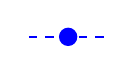
\begin{tikzpicture}[baseline=-0.5ex]
                    \draw[blue,thick,dashed] (0,0) -- (1,0);
                    \draw[blue,fill=blue] (0.5,0) circle (.7ex);
                \end{tikzpicture}
            ),
            Scaling center (
                \tikz[baseline=-0.5ex]\draw[blue] (0,0) circle (0.7ex);
            ).
        }
    \label{iso_fig:circular_hole_mesh}
    \end{figure}

    \begin{figure}
        \begin{subfigure}[b]{1\linewidth}
            \centering
            \scalebox{0.7}{
                % This file was created by matlab2tikz v0.4.6 running on MATLAB 8.2.
% Copyright (c) 2008--2014, Nico Schlömer <nico.schloemer@gmail.com>
% All rights reserved.
% Minimal pgfplots version: 1.3
% 
% The latest updates can be retrieved from
%   http://www.mathworks.com/matlabcentral/fileexchange/22022-matlab2tikz
% where you can also make suggestions and rate matlab2tikz.
% 
%
% defining custom colors
\definecolor{mycolor1}{rgb}{0.00000,0.75000,0.75000}%
\definecolor{mycolor2}{rgb}{0.75000,0.00000,0.75000}%
%
\begin{tikzpicture}

\begin{axis}[%
width=4.52083333333333in,
height=3.5146875in,
scale only axis,
xmode=log,
xmin=10,
xmax=1000,
xminorticks=true,
xlabel={Total DOF},
ymode=log,
ymin=1e-09,
ymax=0.1,
yminorticks=true,
ylabel={Error},
title={L2L Displacement Error},
legend style={draw=black,fill=white,legend cell align=left}
]
\addplot [color=blue,solid,mark=square,mark options={solid}]
  table[row sep=crcr]{
20	0.052647009	\\
40	0.015077369	\\
80	0.004598634	\\
160	0.001317239	\\
};
\addlegendentry{1st order};

\addplot [color=black!50!green,solid,mark=o,mark options={solid}]
  table[row sep=crcr]{
20	0.018330302	\\
40	0.000979438	\\
80	9.0447e-05	\\
160	7.10192e-06	\\
};
\addlegendentry{2nd order};

\addplot [color=red,solid,mark=triangle,mark options={solid,,rotate=180}]
  table[row sep=crcr]{
40	0.001028186	\\
80	6.4874e-06	\\
160	9.03877e-08	\\
};
\addlegendentry{4th order};

\addplot [color=mycolor1,solid,mark=asterisk,mark options={solid}]
  table[row sep=crcr]{
80	8.12048e-06	\\
160	7.13386e-09	\\
};
\addlegendentry{6th order};

\addplot [color=mycolor2,solid,mark=+,mark options={solid}]
  table[row sep=crcr]{
20	0.0371	\\
40	0.00228	\\
80	0.000316	\\
160	2.98e-05	\\
};
\addlegendentry{LNGL 2nd order};

\end{axis}
\end{tikzpicture}%
            }
            \label{iso_fig:circular_hole_displacement_convergence}
            \caption{the relative error in displacement norm $(L^2)$}
        \end{subfigure}
        
        \begin{subfigure}[b]{1\linewidth}
            \centering
            \scalebox{0.7}{
                % This file was created by matlab2tikz v0.4.6 running on MATLAB 8.2.
% Copyright (c) 2008--2014, Nico Schlömer <nico.schloemer@gmail.com>
% All rights reserved.
% Minimal pgfplots version: 1.3
% 
% The latest updates can be retrieved from
%   http://www.mathworks.com/matlabcentral/fileexchange/22022-matlab2tikz
% where you can also make suggestions and rate matlab2tikz.
% 
%
% defining custom colors
\definecolor{mycolor1}{rgb}{0.00000,0.75000,0.75000}%
\definecolor{mycolor2}{rgb}{0.75000,0.00000,0.75000}%
%
\begin{tikzpicture}

\begin{axis}[%
width=4.52083333333333in,
height=3.5146875in,
scale only axis,
xmode=log,
xmin=10,
xmax=1000,
xminorticks=true,
xlabel={Total DOF},
ymode=log,
ymin=1e-05,
ymax=1,
yminorticks=true,
ylabel={Error},
title={L2L Strain Energy Error},
legend style={draw=black,fill=white,legend cell align=left}
]
\addplot [color=blue,solid,mark=square,mark options={solid}]
  table[row sep=crcr]{
20	0.136951345	\\
40	0.070082184	\\
80	0.040238511	\\
160	0.02076975	\\
};
\addlegendentry{1st order};

\addplot [color=black!50!green,solid,mark=o,mark options={solid}]
  table[row sep=crcr]{
20	0.115220087	\\
40	0.0192672307117524	\\
80	0.002314805	\\
160	0.000499173	\\
};
\addlegendentry{2nd order};

\addplot [color=red,solid,mark=triangle,mark options={solid,,rotate=180}]
  table[row sep=crcr]{
40	0.028460196	\\
80	0.001326623	\\
160	6.43781e-05	\\
};
\addlegendentry{4th order};

\addplot [color=mycolor1,solid,mark=asterisk,mark options={solid}]
  table[row sep=crcr]{
80	0.000931962	\\
160	1.04862e-05	\\
};
\addlegendentry{6th order};

\addplot [color=mycolor2,solid,mark=+,mark options={solid}]
  table[row sep=crcr]{
20	0.196598384	\\
40	0.040130929	\\
80	0.00697	\\
160	0.00196	\\
};
\addlegendentry{LNGL 2nd order};

\end{axis}
\end{tikzpicture}%
            }
            \label{iso_fig:circular_hole_energy_convergence}
            \caption{the relative error in the energy norm}
        \end{subfigure}
    \caption{Bending of thick cantilever beam: Convergence results}
    \label{iso_fig:circular_hole_convergence}
    \end{figure}

    \begin{figure}
        \centering
        \scalebox{0.5}{
            \includegraphics{isogeometric_sbfem/images/circular_hole_basis.png}
        }
        \caption{NURBS basis functions and Lagrange basis functions. It can be seen that at Point $B$, the shape functions are continuous}
        \label{iso_fig:circular_hole_basis}
    \end{figure}

    \begin{figure}
        \centering
        \scalebox{0.5}{
            \includegraphics{isogeometric_sbfem/images/circular_hole_shape_function_convergence.png}
        }
        \caption{
            Infinite plate with a circular hole: Convergence results for the relative error in the displacement norm ($L^2$) and
                the relative error in the energy norm. In this case, the arc is represented with NURBS and Lagrange shape functions.
        }
        \label{iso_fig:circular_hole_shape_function_convergence}
    \end{figure}

\pagebreak

\subsection{L-shaped bracket}
\label{subsection:l_shaped_bracket}
\paragraph{}
In this example, consider an L-shaped bracket with isotropic material properties.
Fig. 14 shows the geometry and the boundary conditions of the problem.
The L-shaped bracket is fixed at one end and subjected to downward vertical displacement at the other end.
Plain strain conditions are assumed.
This problem was studied in \cite{LIPTON2010357} by employing the conventional IGA.
In their study, the fillet was modeled as a separate path using biquadratic NURBS with nine control points.
\paragraph{}
In the present study, the control mesh is directly employed for the stress analysis.
However, as the domain does not meet the star convexity, we divide the domain into three sub-domains 
    (see Fig. 14).
We employ NURBS to represent the fillet, whilst for the straight lines, we employ Lagrange basis functions.
The results from the present approach are compared with conventional finite element analysis using the commercial
    software ANSYS$^\circledR$.
\paragraph{}
A total of $2000$ $8$-node quadrilateral elements were used for the finite element analysis.
Fig. 15 shows the von Mises equivalent stress for the L-shaped bracket with and without the fillet.
As expected, the no fillet case shows higher stress when compared to the L-shaped bracket with the fillet.
From Fig. 15, it can be observed that the results from the present approach qualitatively match with the FE solution.
It should be noted that, the proposed method is computationally less intensive than the conventional IGA as it requires
    only the boundary information.



\pagebreak

\subsection{Circular disk with an edge crack in tension}

\paragraph{}
Next, the present formulation is applied to problems with strong discontinuities and singularities.
The unique feature of the proposed framework is that the geometry is exactly represented by using NURBS and the singularities are captured semi-analytically without a priori knowledge of the asymptotic fields.
In the first example, consider a circular disk with an edge crack (see Fig.~\ref{iso_fig:circular_disk_geo_bc}) with Young’s modulus $E=\SI{1}{\newton \per \square \meter}$ and Poisson's ratio $\nu=0.3$.
    \begin{figure}[h!]
        \centering
        \scalebox{0.4}{
            \includegraphics{isogeometric_sbfem/images/circular_disk_geo_bc.eps}
        }
        \caption{Circular disk with an edge crack}
        \label{iso_fig:circular_disk_geo_bc}
    \end{figure}

The analytical displacements solution for mode \RN{1} are given by:
    \begin{subequations}
        \begin{align}
            u_x &= \frac{1}{2}\left[
                \left(
                    \kappa + \frac{n}{2} + (-1)^n
                \right) \cos \left(
                    \frac{n\theta}{2}
                \right) -
                \frac{n}{2} \cos \left(
                    \left(
                        \frac{n}{2} -2
                    \right) \theta
                \right)
            \right]\\
            u_y &= \frac{1}{2}\left[
                \left(
                    \kappa - \frac{n}{2} - (-1)^n
                \right) \sin \left(
                    \frac{n\theta}{2}
                \right) +
                \frac{n}{2} \sin \left(
                    \left(
                        \frac{n}{2} -2
                    \right) \theta
                \right)
            \right]\\
        \end{align}
    \end{subequations}

where $\kappa$ is the Kolosov constant defined in Eq.~\ref{iso_eq:kolosov_constant}.

The analytical stress solution for mode \RN{1} are given by:
    \begin{subequations}
        \begin{align}
            \sigma_{xx} &= \frac{n}{2}\left[
                \left(
                    2 + \frac{n}{2} + (-1)^n
                \right) \cos \left(
                    \left(
                        \frac{n}{2} - 1
                    \right)\theta
                \right) - \left(
                    \frac{n}{2} - 1
                \right)
                \cos \left(
                    \left(
                        \frac{n}{2} -3
                    \right) \theta
                \right)
            \right]\\
            \sigma_{yy} &= \frac{n}{2}\left[
                \left(
                    2 - \frac{n}{2} - (-1)^n
                \right) \cos \left(
                    \left(
                        \frac{n}{2} - 1
                    \right)\theta
                \right) + \left(
                    \frac{n}{2} - 1
                \right)
                \cos \left(
                    \left(
                        \frac{n}{2} -3
                    \right) \theta
                \right)
            \right]\\
            \tau_{xy} &= \frac{n}{2}\left[
                \left(
                    \frac{n}{2} - 1
                \right) \sin \left(
                    \left(
                        \frac{n}{2} - 3
                    \right)\theta
                \right) - \left(
                    \frac{n}{2} + (-1)^n
                \right)
                \sin \left(
                    \left(
                        \frac{n}{2} - 3
                    \right) \theta
                \right)
            \right]
        \end{align}
    \end{subequations}

\paragraph{}
In this example, the circular disk is represented by NURBS.
The control net and the location of control points are shown in Fig.~\ref{iso_fig:circular_disk_mesh} for different NURBS orders.
    \begin{figure}
        \begin{subfigure}[b]{0.5\linewidth}
            \centering
            \scalebox{0.4}{
                \includegraphics{isogeometric_sbfem/images/circular_disk_2nd_9cp.png}
            }
            \caption{9 control points, 2nd order}
        \end{subfigure}
        \begin{subfigure}[b]{0.5\linewidth}
            \centering
            \scalebox{0.4}{
                \includegraphics{isogeometric_sbfem/images/circular_disk_2nd_17cp.png}
            }
            \caption{9 control points, 2nd order}
        \end{subfigure}

        \begin{subfigure}[b]{0.5\linewidth}
            \centering
            \scalebox{0.4}{
                \includegraphics{isogeometric_sbfem/images/circular_disk_3rd_17cp.png}
            }
            \caption{9 control points, 2nd order}
        \end{subfigure}
        \begin{subfigure}[b]{0.5\linewidth}
            \centering
            \scalebox{0.4}{
                \includegraphics{isogeometric_sbfem/images/circular_disk_4th_17cp.png}
            }
            \caption{9 control points, 2nd order}
        \end{subfigure}
        \caption{Meshing of the circular disk with an edge notch}
        \label{iso_fig:circular_disk_mesh}
    \end{figure}

\paragraph{}
The circular disk is subjected to a far field tension and the displacement and the stress modes are computed by the proposed isogeometric SBFEM.
It is noted that only the boundary of the circular disk is discretized using the NURBS and no tensor product of the corresponding knot vectors is required to represent the unknown fields inside the domain.
The convergence of the numerical stress intensity factor (SIF) and the T-stress with mesh refinement is shown in Tab.~\ref{iso_tab:circular_disk_res}.

\begin{table}[]
\caption{T-stress and stress intensity factors for circular disk with an edge crack.}
\label{iso_tab:circular_disk_res}
\begin{tabularx}{\textwidth}{XXXXXXX}
\toprule
    Total    &   \multicolumn{2}{c}{NURBS $p=2$} &\multicolumn{2}{c}{NURBS $p=4$} &\multicolumn{2}{c}{NURBS $p=6$}\\
    \cmidrule{2-7}
    DOF      &   SIF     &   T-stress            &SIF     &   T-stress            &SIF     &   T-stress           \\
    \cmidrule{1-1} \cmidrule{2-3} \cmidrule{4-5} \cmidrule{6-7}
    18       &   2.3520  &   2.9442              &        &                       &        &                      \\
    34       &   2.8693  &   5.1991              &2.8838  &5.4050                 &        &                      \\
    74       &   2.8838  &   5.3112              &2.8840  &5.3445                 &2.8840  &5.3447                \\
    130      &   2.8840  &   5.3318              &2.8840  &5.3444                 &2.8840  &5.3444                \\
\bottomrule
\end{tabularx}
\end{table}

\paragraph{}
It can be seen that with mesh refinement the SIF and the T-stress converge.
Increasing the order of the NURBS functions increases the convergence behavior.
Eq.~\ref{iso_eq:isosbfem_fracture_stress_field} is the parametric equation for the stress field in the polar coordinates $r$ and $\theta$.
The terms $\left(
        r_\eta^{\lambda_i+1}(\eta)
        \boldsymbol{\psi}_{\sigma_i}(\eta)
    \right)$
in Eq.~\ref{iso_eq:isosbfem_fracture_stress_field} together with $\theta(\eta)$ in Eq.~\ref{lr_eq:sbfem_transform} are the stress modes describing the angular distribution at a constant radial coordinate $r$.
For the converged result, Fig.~\ref{iso_fig:circular_disk_modes} shows the displacement and the stress distribution at a constant radial coordinate r around the crack tip for mode \RN{1} fracture.
Each of the stress modes is normalized with its value of $\sigma_{yy}=0^\circ$ .
    \begin{figure}[h!]
        \begin{subfigure}[b]{1\linewidth}
            \centering
            \scalebox{0.4}{
                \includegraphics{isogeometric_sbfem/images/circular_disk_displacement_modes.png}
            }
            \caption{displacements}
        \end{subfigure}
        \begin{subfigure}[b]{1\linewidth}
            \centering
            \scalebox{0.4}{
                \includegraphics{isogeometric_sbfem/images/circular_disk_stress_modes.png}
            }
            \caption{stress}
        \end{subfigure}
    \caption{Displacement and stress modes of circular disk with an edge crack using cubic NURBS functions}
    \label{iso_fig:circular_disk_modes}
    \end{figure}

\paragraph{}
The stress modes from the scaled boundary formulation are compared with the analytical solutions and a very good agreement is observed in Tab.~\ref{iso_tab:circular_disk_res}.
The convergence of the displacement and stress modes with h and p refinement is shown in Fig.~\ref{iso_fig:circular_disk_convergence}.
It can be seen that with refinement the solution converges monotonically.
    \begin{figure}[h!]
        \begin{subfigure}[b]{1\linewidth}
            \centering
            \scalebox{0.65}{
                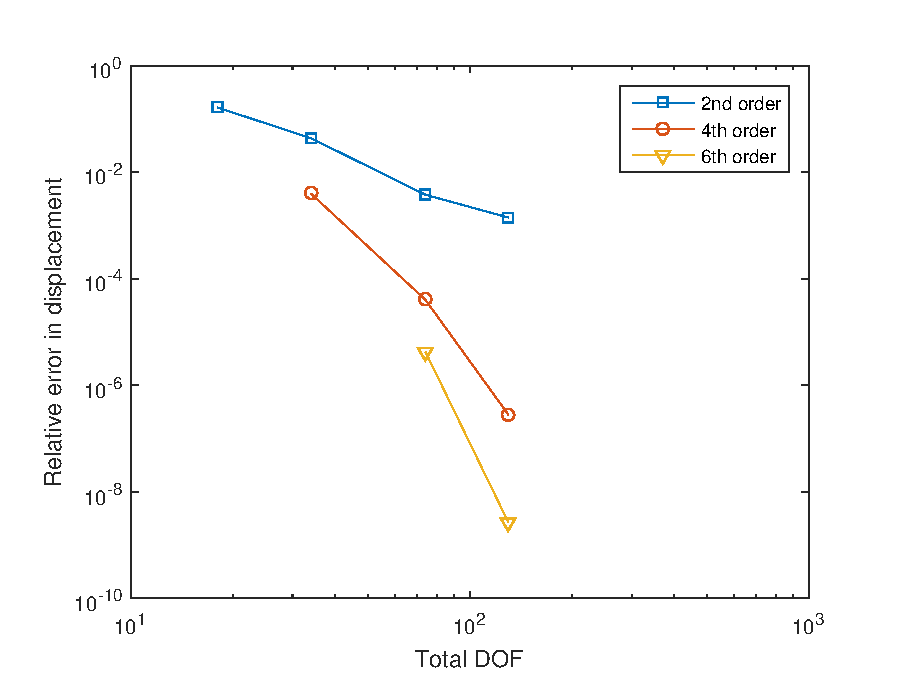
\includegraphics{isogeometric_sbfem/images/circular_disk_convergence_displacement.eps}
            }
            \caption{Displacement mode}
        \end{subfigure}

        \begin{subfigure}[b]{1\linewidth}
            \centering
            \scalebox{0.65}{
                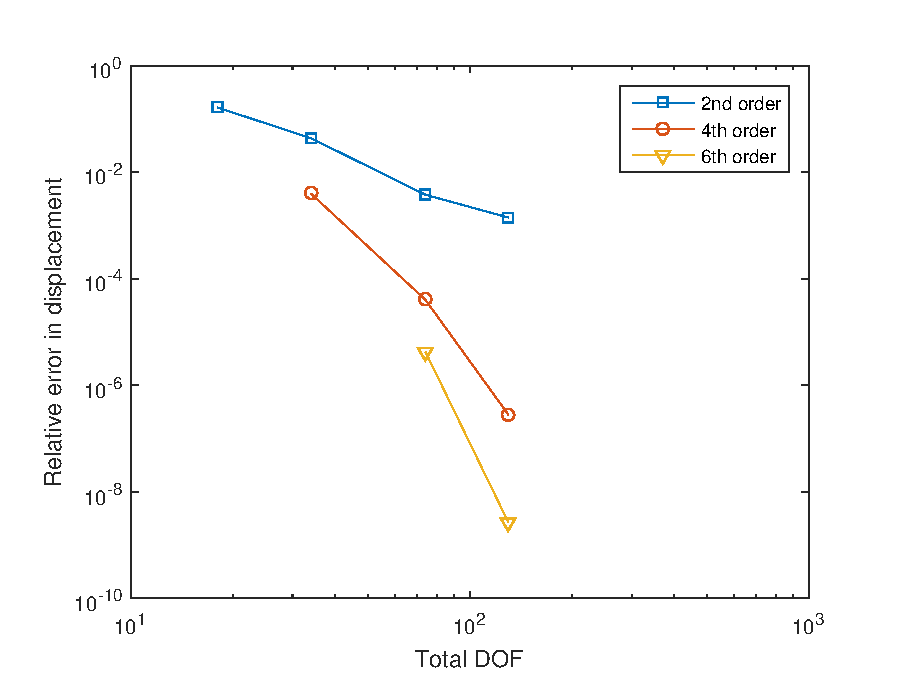
\includegraphics{isogeometric_sbfem/images/circular_disk_convergence_displacement.eps}
            }
            \caption{Displacement mode}
        \end{subfigure}
    \caption{Circular disk with an edge crack: convergence of the displacement mode and stress mode}
    \label{iso_fig:circular_disk_convergence}
    \end{figure}



\subsection{Edge crack in tension}

\paragraph{}
Consider a plate with an edge crack loaded in tension $\sigma=1N/m^2$ over the top and the bottom edges.
The geometry, loading and boundary conditions are shown in fig.~\ref{iso_fig:edge_crack_geo_bc}.
In the figure, $L=2m$ and $H=1m$
The reference mode \RN{1} SIF is given by:
    \begin{equation}
        K_1 = F\left(
            \frac{a}{H}
            \sigma \sqrt{\pi a}
        \label{iso_eq:edge_crack_k1}
        \right)
    \end{equation}
where $a$ is the crack length, $H$ is the plate width, and $F(a/H)$ is an empirical function given by (for $a/H \leq 0.6$)
    \begin{equation}
        F\left( \frac{a}{H} \right) =
            1.12 - 0.231 \left( \frac{a}{H} \right) +
            10.55\left( \frac{a}{H} \right)^2 -
            27.72\left( \frac{a}{H} \right)^3 +
            30.39\left( \frac{a}{H} \right)^4
    \end{equation}

    \begin{figure}
        \centering
        \scalebox{0.4}{
            \includegraphics{isogeometric_sbfem/images/edge_crack_geo_bc.eps}
        }
        \caption{Plate with an edge crack under tension}
        \label{iso_fig:edge_crack_geo_bc}
    \end{figure}

\paragraph{}
The convergence of the mode \RN{1} SIF and the T-stress with mesh size and the order of the NURBS basis function is illustrated in table.~\ref{iso_tab:edge_crack_res}.
It can be seen that decreasing the mesh size and increasing the order of the NURBS basis function, the numerically obtained SIF and the T-stress converge.
\begin{table}
    \caption{Convergence of the mode \RN{1} SIF and T-stress for an edge crack in tension}
    \label{iso_tab:edge_crack_res}
    \begin{tabularx}{\textwidth}{XXXXXXX}
        \toprule
            Total    &   \multicolumn{2}{c}{NURBS $p=2$} &\multicolumn{2}{c}{NURBS $p=4$} &\multicolumn{2}{c}{NURBS $p=6$}\\
            \cmidrule{2-7}
            DOF      &   $K_1$   &   T-stress            &$K_1$   &   T-stress            &$K_1$   &   T-stress           \\
            \cmidrule{1-1} \cmidrule{2-3} \cmidrule{4-5} \cmidrule{6-7}
            62       &   2.7011  &   -0.4137             &2.6647  &-0.4170                &        &                      \\
            98       &   2.7632  &   -0.4210             &2.8343  &-0.4216                &2.8335  &-0.4217               \\
            170      &   2.8028  &   -0.4216             &2.8252  &-0.4217                &2.8245  &-0.4217               \\
            329      &   2.8264  &   -0.4217             &2.8247  &-0.4217                &2.8246  &-0.4217               \\
            eq.~\ref{iso_eq:edge_crack_k1} & 2.8264 & - & & & & \\
        \bottomrule
        \end{tabularx}
\end{table}

\pagebreak

\subsection{Angled crack in an orthotropic body}

\paragraph{}
In this example, consider an orthotropic plate $(b/h = 1)$ with an angled center-crack of length $a/h = 0.5$ under uniform far field tension along the two opposite sides (see fig.~\ref{iso_fig:angled_crack_geo_bc}). 
    \begin{figure}
        \centering
        \scalebox{0.5}{
            \includegraphics{isogeometric_sbfem/images/angled_crack_geo_bc.eps}
        }
        \caption{Angled crack in a rectangular orthotropic body: geometry}
        \label{iso_fig:angled_crack_geo_bc}
    \end{figure}

\paragraph{}
The elastic properties of the material are $E_{11} = E_{22}= E_{33}=15.4\times 10^6 psi$, $G_{12} = G_{23} = G_{13} = 15.7 \times 10^6 psi$, and $\nu_{12} = \nu_{23} = \nu_{13} = 0.4009$.
The results are compared with those obtained in \cite{Banks2005}.
The convergence of mode \RN{1} and mode \RN{2} SIF with mesh size is shown in tab.~\ref{iso_tab:angled_crack_convergence} for a crack at an angle $\alpha = \pi/12$.
The influence of the order of the shape functions is also shown.
It can be seen that increasing the number of degrees of freedom, the error in the numerical SIF decreases.
A very good agreement is observed.
\begin{table}
\caption{Convergence of the generalized stress intensity factors $
    (\mean{K_\RN{1}}, \mean{K_\RN{2}}) =
    (K_\RN{1},K_\RN{2}) /
    P\sqrt(\pi a)
    $}
\label{iso_tab:angled_crack_convergence}
\begin{tabularx}{\textwidth}{XXXXX}
    \toprule
    \multirow{2}{*}{Order}& & \multicolumn{3}{c}{Number of DOF} \\
    \cmidrule{3-5}
    & & 160 & 240 & 320 \\
    \multirow{2}{*}{$2$}    &   $\mean{K_\RN{1}}$   &   1.2770  &   1.2723  &   1.2706  \\
                            &   $\mean{K_\RN{2}}$   &   0.2918  &   0.2915  &   0.2913  \\
    \multirow{2}{*}{$4$}    &   $\mean{K_\RN{1}}$   &   1.2700  &   1.2697  &   1.2697  \\
                            &   $\mean{K_\RN{2}}$   &   0.2914  &   0.2913  &   0.2913  \\
    \multirow{2}{*}{$6$}    &   $\mean{K_\RN{1}}$   &           &   1.2668  &   1.2670  \\
                            &   $\mean{K_\RN{2}}$   &           &   0.2913  &   0.2913  \\                           
    \midrule
    \bottomrule
\end{tabularx}
\end{table}

\paragraph{}
Also, increasing the order of the NURBS basis functions, the error decreases.
The influence of the crack orientation α on the mode \RN{1} and mode \RN{2} SIF is shown in tab.~\ref{iso_tab:angled_crack_sif_1} and tab.~\ref{iso_tab:angled_crack_sif_2}.
A total of 80 control points are used with different order of the NURBS basis functions.
It can be seen that a very good agreement is observed.
\begin{table}
\caption{Generalized stress intensity factors $K_\RN{1}/P\sqrt{\pi a}$ of angled crack in rectangular orthotropic body}
\label{iso_tab:angled_crack_sif_1}
\begin{tabularx}{\textwidth}{XXXXX}
    \toprule
    Angle   &   $K_\RN{1}$  &   \multicolumn{3}{c}{ }  \\
    \cmidrule{2-5} 
    $\alpha$&\cite{Banks2005}&  \multicolumn{3}{c}{Order of the curve}  \\
    \cmidrule{3-5} 
    & & 2 & 4 & 6 \\
    \midrule
    0         & 1.3755 & 1.3603 & 1.3583 & 1.3583 \\
    $\pi/12 $ & 1.2692 & 1.2706 & 1.2697 & 1.2670 \\
    $\pi/ 6 $ & 1.0268 & 1.0277 & 1.0270 & 1.0270 \\
    $\pi/ 4 $ & 0.6952 & 0.6941 & 0.6944 & 0.6943 \\
    $\pi /3 $ & 0.3579 & 0.3582 & 0.3580 & 0.3580 \\
    $5\pi/12$ & 0.1095 & 0.0996 & 0.1003 & 0.1004 \\
    \bottomrule
\end{tabularx}
\end{table}

\begin{table}
    \caption{Generalized stress intensity factors $K_\RN{2}/P\sqrt{\pi a}$ of angled crack in rectangular orthotropic body}
    \label{iso_tab:angled_crack_sif_2}
    \begin{tabularx}{\textwidth}{XXXXX}
        \toprule
        Angle   &   $K_\RN{2}$  &   \multicolumn{3}{c}{ }\\
        \cmidrule{2-5}
        $\alpha$&\cite{Banks2005}&  \multicolumn{3}{c}{Order of the curve}\\
        \cmidrule{3-5}
        & & 2 & 4 & 6 \\
        \midrule
        0         & 0.0000 & 0.0000 & 0.0000 & 0.0000 \\
        $\pi/12 $ & 0.2912 & 0.2914 & 0.2913 & 0.2913 \\
        $\pi/ 6 $ & 0.5092 & 0.5087 & 0.5093 & 0.5092 \\
        $\pi/ 4 $ & 0.5807 & 0.5948 & 0.5946 & 0.5946 \\
        $\pi /3 $ & 0.5248 & 0.5247 & 0.5248 & 0.5248 \\
        $5\pi/12$ & 0.3108 & 0.3119 & 0.3117 & 0.3117 \\
        \bottomrule
    \end{tabularx}
\end{table}

\pagebreak

\subsection{Transient analysis of bimaterial plate with a notch}

\pagebreak

%=================================================================================================================================%
\section{Conclusions}
\paragraph{}
In this chapter, the NURBS basis functions are employed to approximate the unknown fields in the circumferential direction within the framework of the SBFEM.
The accuracy, effectiveness and the convergence properties of the proposed method are demonstrated with benchmark problems in linear elasticity and linear elastic fracture mechanics.
From the numerical studies, it can be observed that the NURBS basis functions yield superior accuracy when compared to Lagrange basis functions of the same order.
The proposed method overcomes the disadvantages of both the isogeometric finite element analysis and the isogeometric boundary element method. 
Like in the IGAFEM no fundamental solution is required and like in the IGABEM the spatial dimension is reduced by one.
However, for complicated geometries, to meet the star convexity, subdivision into smaller sub-domains is required.
When applied to problems with singularities, the proposed method does not require additional functions to span the solution space.
Moreover, the proposed framework does not require internal discretization to study the dynamic response at high frequencies.
    % chapter 3
%!TEX root = ../thesis.tex
\chapter{Quad-tree mesh in 2D analysis}
\label{qdt_sec:main}
\section{Introduction}
\paragraph{}
The main objective of this chapter is to implement an adaptor that can parse the geometric information in CAD directly and to develop an automatic mesh generation algorithm based on it.
The IGES file introduced in Sec.~\ref{lr_sec:IGES} is used in the proposed method as the bridge between the CAD and the numerical analysis.
A quad-tree mesh generation algorithm described in \hl{Sec.}~\ref{qt_sc:quadtree} will be adopted to generate a high quality mesh \hl{that meets the scaling requirement discussed in Sec}.~\ref{lr_sec:sbfem}.
Either the NURBS basis function or the traditional shape function can be used as the shape function of the SBFEM solver.
The geometric boundary will be translated into polylines before the meshing and the intersections are calculated based on them.
Intersecting points on these polylines are projected back to the NURBS surface after the meshing is generated to retain the exact geometry.
% We further extend the method to problems with singularities within the framework of linear elastic fracture mechanics.
The proposed method enhances the conventional SBFEM and the salient features of the method are:
    \begin{itemize}
        \item Direct using design file as geometric input\hl{s}
        \item No human effort involvement in mesh generation
        \item Retained exact geometry
        \item High quality mesh generated from the quad-tree algorithm
    \end{itemize}
\paragraph{}
This chapter is organized as follows.
The CAD output (iges file) will be introduced first.
After that, an overview of the algorithm that can generate quadtree mesh will be provided.
Furthermore, a point projection method for NURBS curve utilizing its strong convex hull property is presented.
The accuracy and the convergence properties of the proposed techniques are demonstrated with benchmark problems in the context of linear elasticity, followed by concluding remarks in the last section.


\section{CAD output in 2D}
\label{qt_sc:iges}
\paragraph{}
The IGES\cite{IGES1983} files introduced in Sec.~\ref{lr_sec:IGES} are used as the bridge between the engineering design and the numerical analysis in the proposed method.
As a standard file format in engineering design industry, it is supported by almost all design softwares all over the world.
Consequently, it offers a possibility to minimize the human effort spent on mesh generation.

\subsection{Parse geometry in IGES file}
\paragraph{}
The IGES file provides all information that describe the geometric input.
Abstract structure of the IGES file that describe the 2D geometry can be regarded as a simple curve-surface structure.
In other words, it defines the geometric input as certain number of surfaces with their boundaries in different colors, which represent different materials in engineering practice.
Each surface contains a list of curve indices which are corresponding to the curve information described in IGES file.

\paragraph{}
When the IGES file is feed into the programme, each line in the directory entry will be parsed entity by entity.
Parameter in directory entry describe the type and reference to other useful values for the entity.
An entity may refer to one or many entities in directory entry.
Detail of the specification of each entity is explained in \cite{Nasr2007} in detail.

%=====================================================================================================================%
\subsection{Output to mesh generator}
\label{qdt_section:iges_output}
\paragraph{}
The output file that the mesh generator read in will be a shorter summary of the geometric input.
Boundary representation will be kept as the data structure to describe the geometric input.
However, some fields apart from the curves or the surfaces will be added.
In the output file, the geometry will be organized in key points, polylines and surfaces.
The key points define the coordinates of all points and polylines are used to represent all curves including NURBS curves for simplification.
NURBS curves introduced in in \ref{lr_sec:NURBS} can be used directly by the mesh generator as well but it is found that the computational cost in the calculation of the distance between points to NURBS curves surpasses the merits of using it directly.
The exact geometry can be retained by projecting the nodes on the boundary back to the origin NURBS curves at the end of the algorithm.

\paragraph{}
Representing a straight line with polyline can be natural, first and the last points will be enough to achieve an exact representation.
However, that is not the case for curves whose curvature is not always zero.
Although adding more key points can increase the quality of polyline representation, computational cost in calculating the distance increases at the same time.
Yet, having only few key points may result in a bad polyline representation which leads to a poor mesh quality.
Elements may be twisted after the nodes on the boundary are projected to the origin curves.
As a consequence, a quantified indicator that is able to control the number and the position of the vertices on the polyline can be necessary.

%=====================================================================================================================%
\subsection{Discretization of the circular arc}
\paragraph{}
The chord ratio can be a good indicator for circular arc.
The arc length to chord length ratio $\frac{a}{L}$ illustrated in Fig.~\ref{qt_fig:iges_chord_ratio} can be expressed in angle $\alpha$ as:
    \begin{equation}
        \frac{a}{L} = \frac{
            \sqrt{2-2\cos\alpha}
        }{\alpha}
        = \frac{
            2\sin\frac{\alpha}{2}
        }{\alpha}
    \end{equation}
%
The maximum angle $\alpha$ satisfy arc length to chord length ratio $\frac{a}{L} > 1-\epsilon$ with $
    \sin\frac{\alpha}{2} = 1 - \frac{x^3}{6} + O(x^7)
$ can be derived as:
    \begin{equation}
        \alpha < \sqrt{24 \epsilon}
    \end{equation}

    \begin{figure}[h!]
        \centering
        \scalebox{1}{
            \includegraphics{quadtree/images/iges_chord_ratio.eps}
        }
        \caption{Chord length for circular arc}
        \label{qt_fig:iges_chord_ratio}
    \end{figure}
%
%=====================================================================================================================%
\subsection{Discretization of the NURBS curve}
\paragraph{}
For NURBS curves who have no closed form chord ratio, similar idea can be applied numerically.
The NURBS curve is first divided into serval smaller ones based on the knot vector as described in Sec.~\ref{lr_sec:nurbs_knot_ins}.  % may be explained in detail
Since the order of each subdivided NURBS curve used in engineering softwares are predominantly lower or equal to three, the sub-curves then can be divided into two classes, convex curves or concave curves with an inflection point as shown in Fig.~\ref{qt_fig:iges_chord_ratio_nurbs}.
    \begin{figure}
        \begin{subfigure}[b]{0.5\linewidth}
            \centering
            \scalebox{0.5}{
                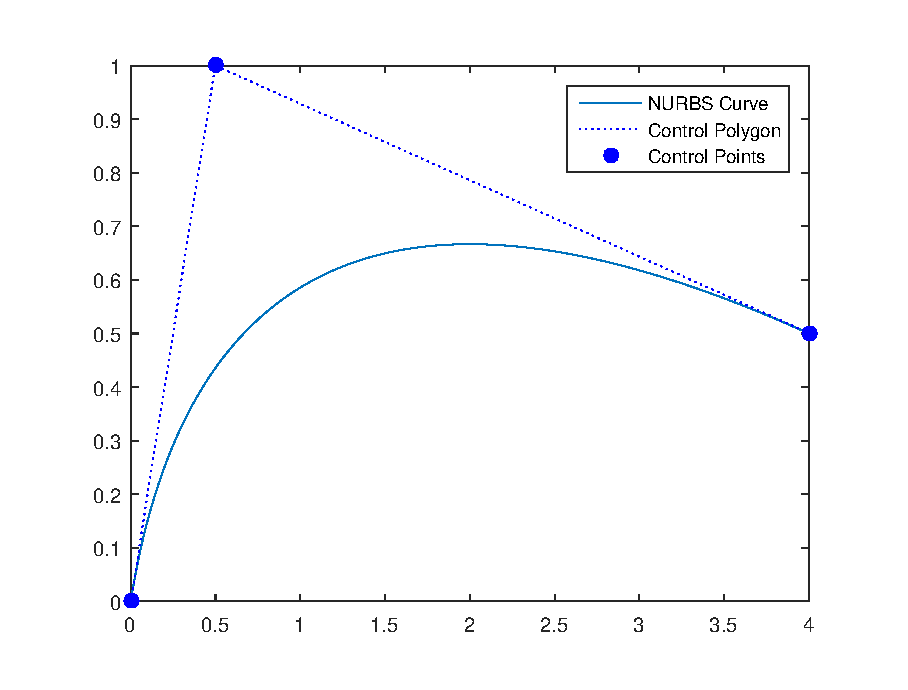
\includegraphics{quadtree/images/iges_chord_ratio_nurbs_convex.eps}
            }
            \caption{Convex}
        \end{subfigure}
        \begin{subfigure}[b]{0.5\linewidth}
            \centering
            \scalebox{0.5}{
                \includegraphics{quadtree/images/iges_chord_ratio_nurbs_concave.eps}
            }
            \caption{Concave with an inflection point}
        \end{subfigure}
    \caption{Type of sub-devided NURBS curves: convex and concave with an inflection point}
    \label{qt_fig:iges_chord_ratio_nurbs}
    \end{figure}
%
In order to determine the target NURBS curve is convex one or concave one, a cross product will be conducted.
by assuming the subdivided NURBS curve is cubic, there will be four control points $P_1,P_2,P_3$ and $P_4$.
If the signs of $cross(\overrightarrow{P_1P_2},\overrightarrow{P_2P_3})$ and $cross(\overrightarrow{P_1P_2},\overrightarrow{P_2P_3})$ are the same, then the curve is convex.
Otherwise it will be concave.

%=====================================================================================================================%
\subsubsection{Convex curves}
\label{qt_ssc:convex_curves}
\paragraph{}
Start with the simple case, in the situation illustrated in Fig.~\ref{qt_fig:iges_chord_split_convex_sum} where line $C(u_0)C(u_n)$ and the NURBS curve form a convex set, we are looking for a point $C(u_m)$ on the curve so that $C'(u_m)$ is parallel to $\overrightarrow{C(u_0)C(u_n)}$
    \begin{figure}[h!]
        \centering
        \scalebox{0.6}{
            \includegraphics{quadtree/images/iges_chord_split_convex_sum.eps}
        }
        \caption{Discretization for convex NURBS curve}
        \label{qt_fig:iges_chord_split_convex_sum}
    \end{figure}
%
The target is to split one NURBS curve segment into two.
The splitting will be processed until the arc length to chord length ratio of any splitted curves are smaller than the tolerance.
Based on the property of the convex set, there can be one and only one parameter $u_m$ that satisfies the condition.
As a consequence, numerical methods such as Newton's method can be adopted to determine it.
For a given $u_m$, the next iteration will be:
    \begin{equation}
        u_{m_{new}} =  u_n - \frac{f(u_m)}{f'(u_m)}
    \end{equation}
%
where 
    \begin{equation}
        f(u) = C'(u) \begin{bmatrix}
            - C_y(u_n) + C_y(u_0) \\
            C_x(u_n) - C_x(u_0)
        \end{bmatrix}
    \end{equation}
%
The procedure to find $u_m$ can be concluded in Algorithm.~\ref{qdt_alg:split_convex_nurbs} and Algorithm.~\ref{qdt_alg:discrete_convex_nurbs} describes the procedure to find all knots corresponding to the vertexes of the polylines recursively.
\begin{algorithm}
    function splitConvexCurve(curve,u\_0, u\_n) \\
    \Input{
        curve, the input NURBS curve \\
        u\_0,u\_n, two end knots of the NURBS curve
    }
    \Output{
        u\_m, in Fig.~\ref{qt_fig:iges_chord_split_convex_sum}
    }
    u\_m = (u\_n + u\_0) * 0.5 \\
    pt\_0, pt\_n = getCurvePts(u\_0, u\_n) \\
    vector\_0n = Vector(pt\_0,pt\_n) \\
    angle = vector\_0n.atan2() \\
    deri1\_m = getCurveDeri(u\_m,1) \\
    angle\_m = deri1\_m.atan2() \\
    \While{abs(angle\_m-anlge)$<10^{-4}$}
      {
        deri1\_m, deri2\_m = getCurveDeri(u\_m,2) \\
        angle\_m = atan2(deri1\_m.y, deri1\_m.x)  \\
        fu = deri1\_m * vector\_0n.normalVector() \\
        fu\_deri = deri2\_m * vector\_0n.normalVector() \\
        u\_m = u\_m - fu / fu\_deri \\
        deri1\_m = getCurveDeri(u\_m,1) \\
        angle\_m = deri1\_m.atan2()
      }
    \caption{Split a convex NURBS curve into two}
    \label{qdt_alg:split_convex_nurbs}
\end{algorithm}
%
%
\begin{algorithm}
    function discreteConvexCurve(curve,eps,u\_0,u\_n,u)
    \Input{
        curve, the input NURBS curve \\
        eps, the tolerance of the chord to arc-length ratio \\
        u\_0,u\_n, two end knots of the NURBS curve
    }
    \Output{
        u, the vector of the knot corresponding to vertexes of the polylines
    }
    arcLength = curve.arcLength(u\_0,u\_n) \\
    chordLength = curve.getPt(u\_0).distanceTo(curve.getPt(u\_n)) \\
    \eIf{1-chordLength/arcLength $<$ eps}{
        return
    }{
        u\_m = (splitConvexCurve(curve,u\_0,u\_n))
        u.add(u\_m)
        discreteConvexCurve(curve,eps,u\_0,u\_m)
        discreteConvexCurve(curve,eps,u\_m,u\_n)
        return
    }    
\caption{Discrete a convex NURBS curve recursively}
\label{qdt_alg:discrete_convex_nurbs}
\end{algorithm}
%=====================================================================================================================%
\subsubsection{Concave curves}
\paragraph{}
As can be seen in Fig.~\ref{qt_fig:iges_chord_ratio_nurbs}, the extracted cubic NURBS curve will have no more than one inflection point.
The reason for that is because the target function is cubic and hence its second derivative will be in first order.
Consequently, numerical methods such as Newton's method can be used to find this unique point.
After that, the curve can be divided into two convex ones and the algorithms introduced in \ref{qt_ssc:convex_curves} can be used separately.
The Newton's iteration can be written as
    \begin{equation}
        u_{n_{new}} = u_n - \frac{f(u_n)}{f'(u_n)}
    \end{equation}

where
    \begin{equation}
        f(u) = C''(u)
    \end{equation}
%
%=====================================================================================================================%
\subsubsection{Calculation of the arc length}
\paragraph{}
The arc length of the NURBS curve defined on $u \in [u_0, u_n]$ can be expressed as
    \begin{equation}
        L = \int_{u_0} ^{u_n} \sqrt{C_x^2(u) + C_y^2(u)} du
    \end{equation}
%
The integration can be solved by the help of the numerical integration quadrature described in \ref{iso_section:numerical_integration} as:
    \begin{equation}
        L = \sum_{i=0}^n a_i \sqrt{C_x^2(u_i) + C_y^2(u_i)}
    \end{equation}


\section{Quad-tree structure}
\label{qt_sc:quadtree}
\paragraph{}
After the geometry information is exported from the IGES file, it can be feed into the quad-tree algorithm to generate mesh of the problem domain.
As an algorithm based on computational geometry, it require great amount of numerical operation and hence the result may be sensitive to the tolerance.
An absolute tolerance may not be able to handle problem with very large or small geometric size.
As a consequence, the first step is to normalize the geometry into a uniform space ($10\times10$ is used in this chapter).

\subsection{Background mesh}
\paragraph{}
Background mesh, like its name, describe a mesh in the background. %fig
Its density is decided by the geometry.
This section will introduce the procedure to generate the background mesh.
\paragraph{}
First of all, we start with one square which is the root of the tree.
The size of it will be slightly larger than the normalized input geometry and it is selected as $16 \times 16$ in this chapter.
After that, the root square will be divided into millions (defined by resolution, defined as $2^{res} \times 2^{res}$) smaller ones like pixel in the image.
Then, $2^{s_{max}} \times 2^{s_{max}}$ pixels will be group into the first layer of the tree, or initial background mesh.
It is used to control the maximum allowable mesh size globally or separately for different material regions.
There are two ways to decided whether each individual square need to be refined or not, seed points method and curve size field and both of them will be used depends on the requirement of the controlling over the mesh.

\paragraph{}


\subsection{Hardpoint treatment}

\subsection{Bucket sort algorithm}

\subsection{Cutting with boundary}

\subsection{Color the region}


\section{Points projection}
\label{qt_sc:projection}
\subsection{Projection algorithm}
\paragraph{}
Point projection algorithm is to find the nearest point in parameter $(u)$ on the NURBS curve of the test point.
In the proposed method, all points on the NURBS curve is generated based on the approximated polylines and hence are not exactly on the boundaries.
Although there exists a closed form solution for point projection, it require the order of the NURBS curve must be less than $4$ \citep{Pie1997}.
As a consequence, a projection algorithm \citep{MA200379} using Newton-Raphson method is introduced to tackle this problem.

\paragraph{}
For a given point $P=(x,y)$, its projection on the curve $C(u$ so that the distance $|P-C(u)|$ is minimum is targeted.
However, in the proposed method, the existence of the large number of the possible curves increase the computational cost significantly.
The projection point for the test point $P$ need to be determined for every existing curves and the one with the smallest minimum distance will be selected.
One possible improvement could be limit the possible curves to only a few by utilizing the fact that the NURBS curves has been divided into multiple sub-curves without interior knot by knot insertion introduced in Sec.~\ref{lr_sec:nurbs_knot_ins}
Another property that can be utilized is that most of the test point $P$ is expected to be extremely close to its projection on the curve $C(u)$.

\paragraph{}
As a consequence, the strong convex hull property can be adopted to limit the number of possible curves to less than $2$.
The building of the convex hull is explained in detail in Sec.~\ref{qdt_sc:convex_hull}.
The signed distance of the test point to all curves' convex hull is calculated and only the curves with negative signed distance which indicate that the point is in the convex hull will be selected as candidates.
If no negative distance is detected, a few number (taken as $3$ in the proposed method) of curves with minimum signed distance will be selected.

\paragraph{}
In order to find the projection of the test point $P$ on the curve $C$, target function $f$ can be expressed as
\begin{equation}
    f(u) = \mathbf{C}^\prime (u) \cdot (\mathbf{C}(u) - \mathbf{P})
\end{equation}
%
When $f(u)$ gives $0$, the point either located on the curve or the distance $|\mathbf{C}(u) - \mathbf{P}|$ is minimal.
and two scalars $f$ and $g$ are defined as
%
The iteration can be concluded as
\begin{equation}
    u_{i+1} = u_i -
    \frac{ f(u_i) }{ f^\prime(u_i) }
\label{qdt_eq:projection_iteration}
\end{equation}
After one iteration is finished, the following criteria are checked in sequence.
\paragraph{1}
Is the point coincide with $C(u_i)$
\begin{equation*}
    |\mathbf{C} (u_i) - \mathbf{P}| \leq \epsilon_1
\end{equation*}
%
where $\epsilon_1$ stands for the tolerance for distance in Euclidean space.
\paragraph{2}
Is the cosine zero
\begin{equation*}
    \frac{
        |\mathbf{C}^\prime (u) \cdot (\mathbf{C}(u) - \mathbf{P})|
    }{
        |\mathbf{C}^\prime (u)|
        |\mathbf{C}(u) - \mathbf{P}|
    } \leq \epsilon_2
\end{equation*}
%
where $\epsilon_2$ stands for the tolerance for cosine.
If either of these conditions are met, the iteration is terminated.
Otherwise Eq.~\ref{qdt_eq:projection_iteration} is performed to find the parameter $u_{i+1}$ for next iteration.
\paragraph{3}
Make sure $u$ and $v$ are within there domains
\begin{equation*}
    u_{i+1} \in [a,b]
\end{equation*}
%
where $a$ and $b$ are the lower and upper bounds for the knot vector of curve $C$.
If the curve is open
\begin{equation}
    \left\{
        \begin{array}{rl}
            u_{i+1} = a & u_{i+1} < a \\
            u_{i+1} = b & u_{i+1} > b
        \end{array}
    \right.
\end{equation}
%
If the curve is closed
\begin{equation}
    \left\{
        \begin{array}{rl}
            u_{i+1} = b - ( a - u_{i+1} ) & u_{i+1} < a \\
            u_{i+1} = a + ( u_{i+1} - b ) & u_{i+1} > b
        \end{array}
    \right.
\end{equation}
%
\paragraph{4}
The difference between the new parameter $u_{i+1}$ and the old one $u_i$ is insignificant
\begin{equation*}
    |
        (u_{i+1} - u_i)\mathbf{C}^\prime(u_i)
    |
    \leq \epsilon_1
\end{equation*}
The iteration will be terminated if this condition is meet.



\subsection{Convex hull in 2D}
\label{qdt_sc:convex_hull}
\paragraph{}
The convex hull property of the NURBS curve indicates that all points on the curve must be contained within the convex hull constructed by its control points \citep{SELIMOVIC2009772}
There are great number of algorithm that can be used including gift wrapping \citep{Cormen:2009:IAT:1614191}, graham scan \citep{ANDERSON197853}, quick hull \citep{Barber:1996:QAC:235815.235821}, Chan's algorithm \citep{Chan1996} and so on \citep{doi:10.1137/0215021, ANDREW1979216}.
The quick hull is adopted in the proposed as it provides a computationally efficient and stable algorithm.
The algorithm utilize the idea of `` divide and conquer'' to build the convex hull with an expected time complexity of $O(nlog(n))$ and  $O(n^2)$ for the worst case.
Generally speaking, it works as expected in most of the situation except for the case of high symmetry or most of the points located at the circumference of a circle.
The algorithm can be implemented with following steps:
\begin{enumerate}
    \item Find the most left and right points (points with minimal and maximum $x$) since they are proved to be part of the convex hull.
    \item Connect these two points and use the line to separate other points into two group.
    \item Find the point with maximum distance to the line in step 2 in any group.
    \item Construct a triangle with two points in step 2 and the point in step 3.
    \item Eliminate all points contained by these two subsets in step 4.
    \item Repeat the previous three steps and the distance calculated in step 2 is determined as the point to the triangle instead of the line in step 1.
    \item Terminate the iteration when no points are left
\end{enumerate}


\section{Numerical Examples}
\subsection{Cantilever beam}
\paragraph{}
A two-dimensional cantilever beam subjected to a parabolic shear load at the free end is examined as shown in Fig.~\ref{qdt_fig:ex_cantilever_beam_geo_bc}.
    \begin{figure}[h!]
    \centering
        \scalebox{0.6}{\includegraphics{isogeometric_sbfem/images/cantilever_beam_geo_bc.eps}}
        \caption{ Cantilever beam: Geometry and boundary conditions.}
        \label{qdt_fig:ex_cantilever_beam_geo_bc}
    \end{figure}
%
The geometry is: length $L=8m$, height $D=4m$.
The material properties are: Young’s modulus $E$ = $3 \times 10^7 N/m^2$ , Poisson’s ratio $ \nu =0.25$.
The parabolic shear force is $P = 250 N$.
The exact solutions for the displacements are given by \citep{Aug2008} as Eq.~\ref{iso_eq:cantilever_beam_displacement_solution}.
where $I=D^3/12$ is the moment of inertia, $\mean{E}=E$, $\mean{\nu}=\nu$ and $\mean{E}=E/(1-\nu^2)$, $\mean{\nu}=nu/(1-nu)$ for plane stress and plane strain condition respectively.
The stress $\sigma$ can be expressed as \citep{Aug2008} as Eq.~\ref{iso_eq:cantilever_beam_stress_solution}.
The strain energy can be derived from Eq.~\ref{iso_eq:cantilever_beam_stress_solution} and Eq.~\ref{iso_eq:cantilever_beam_displacement_solution} as Eq.~\ref{iso_eq:cantilever_beam_energy_solution}.

\paragraph{}
In this example, rigid body motion is constrained by fixing 3 DOF on the left edge of the beam.
$u_x=0$ for points at $(0,-D/2)$ and $(0,D/2)$ and $u_y =0$ for point at $(0,0)$.
Stress from analytical solution in Eq.~\ref{iso_eq:cantilever_beam_stress_solution} are applied on the boundaries.

\paragraph{}
Due to the fact that the geometry of the cantilever beam can be described by four points and four straight lines, drawing in AutoCAD may not be necessary.
As a result, the input geometry is defined manually.
Generated background mesh, coloring and the final result with $res=32$, $s_{max}=16$ and $s_{min}=1$ are shown in Fig.~\ref{qdt_fig:ex_cantilever_beam_background_mesh}, Fig.~\ref{qdt_fig:ex_cantilever_beam_mesh_coloring} and Fig.~\ref{qdt_fig:ex_cantilever_beam_mesh_final}.

    \begin{figure}
        \centering
        \scalebox{0.4}{
            \includegraphics{quadtree/ex_images/cantilever_background_mesh.eps}
        }
        \caption[Background mesh of cantilever beam]{Background mesh of cantilever beam : Bold lines represents the input geometry}
        \label{qdt_fig:ex_cantilever_beam_background_mesh}
    \end{figure}

    \begin{figure}
        \centering
        \scalebox{0.4}{
            \includegraphics{quadtree/ex_images/cantilever_coloring.eps}
        }
        \caption[Mesh coloring of cantilever beam]{Mesh coloring of cantilever beam : Grey area represents the cantilever beam}
        \label{qdt_fig:ex_cantilever_beam_mesh_coloring}
    \end{figure}

    \begin{figure}
        \centering
        \scalebox{0.3}{
            \includegraphics{quadtree/ex_images/cantilever_final_mesh.eps}
        }
        \caption[Final mesh of cantilever beam]{Final mesh of cantilever beam}
        \label{qdt_fig:ex_cantilever_beam_mesh_final}
    \end{figure}
% DOF err
% 146 - 0.019587 (32,16)
% 178 - 0.0082845 (32,2)
% 438 - 0.0027044 (64,2)
% 1658- 0.00066929 (128,2)
Mesh with different parameters are plotted in Fig.~\ref{qdt_fig:ex_cantilever_mesh_all} and the convergence study is plotted in Fig.~\ref{qdt_fig:ex_cantilever_mesh_conv}

    \begin{figure}[h!]
        \begin{subfigure}[b]{1\linewidth}
            \centering
            \scalebox{0.4}{
                \includegraphics{quadtree/ex_images/qdt_cantilever_mesh_178.eps}
            }
            \caption{Mesh with $res=32$, $s_{max}=2$, 178 DOFs}
        \end{subfigure}
        \\
        \begin{subfigure}[b]{1\linewidth}
            \centering
            \scalebox{0.4}{
                \includegraphics{quadtree/ex_images/qdt_cantilever_mesh_438.eps}
            }
            \caption{Mesh with $res=64$, $s_{max}=2$, 438 DOFs}
        \end{subfigure}
        \\
        \begin{subfigure}[b]{1\linewidth}
            \centering
            \scalebox{0.4}{
                \includegraphics{quadtree/ex_images/qdt_cantilever_mesh_1658.eps}
            }
            \caption{Mesh with $res=128$, $s_{max}=2$, 1658 DOFs}
        \end{subfigure}
        \caption[Mesh of the cantilever beam]{Mesh of the cantilever beam}
        \label{qdt_fig:ex_cantilever_mesh_all}
    \end{figure}


    \begin{figure}[H]
        \centering
        \scalebox{0.6}{
            \includegraphics{quadtree/ex_images/qdt_cantilever_conv.eps}
        }
        \caption[Convergence of the cantilever beam]{Convergence of the cantilever beam}
        \label{qdt_fig:ex_cantilever_mesh_conv}
    \end{figure}

    

\subsection{Infinite plate with a circular hole}
\paragraph{}
In this example, an infinite plate with a traction free hole under uniaxial tension $(\sigma = 1 N/m^2 )$
along x-axis (see fig.~\ref{iso_fig:circular_hole_geo_bc}) is considered.

    \begin{figure}[h!]
        \centering
        \scalebox{0.75}{
            \includegraphics{isogeometric_sbfem/images/circular_hole_geo_bc.eps}
        }
        \caption{ Infinite plate with a circular hole: geometry and boundary conditions}
        \label{qdt_fig:circular_hole_geo_bc}
    \end{figure}
    
The exact solution of the principal stresses in Cartesian coordinate $(r,\theta)$ is given by \cite{Sukumar2001} in eq.~\ref{iso_eq:ex_chole_stress_sol}.

\subsection{Plane strain bracket}
\paragraph{}
In this example, a plane strain bracket with a downward uniform distributed load on the top is considered (see Fig.~\ref{qdt_fig:ex_bracket_geo_bc}).
The material properties are: Young’s modulus $E = 2\times 10^5 N/m^2$ and Poisson’s ratio $\nu = 0.3$.
    \begin{figure}[H]
        \centering
        \begin{subfigure}[b]{1\linewidth}
            \centering
            \scalebox{1.2}{
                \includegraphics{quadtree/ex_images/ex_bracket_geo.eps}
            }
        \end{subfigure}
        \begin{subfigure}[b]{1\linewidth}
            \centering
            \scalebox{1.3}{
                \includegraphics{quadtree/ex_images/ex_bracket_load.eps}
            }
        \end{subfigure}
        \caption{ Plane strain bracket: geometry and boundary conditions}
        \label{qdt_fig:ex_bracket_geo_bc}
    \end{figure}

\paragraph{}
A total strain energy of $282.927$ is determined by ANSYS with the mesh shown in Fig.~\ref{qdt_fig:ex_bracket_ansys_mesh}
    \begin{figure}[H]
        \centering
        \scalebox{0.35}{
            \includegraphics{quadtree/ex_images/ex_bracket_ansys_mesh_31002nodes.png}
        }
        \caption{ANSYS mesh for plane strain bracket (62004 DOF)}
        \label{qdt_fig:ex_bracket_ansys_mesh}
    \end{figure}
%
Drawing in AutoCAD will be divided into two parts: base and the holes as shown in Fig.~\ref{qdt_fig:ex_bracket_cad}
    \begin{figure}[H]
        \centering
        \begin{subfigure}[b]{1\linewidth}
            \centering
            \scalebox{0.4}{
                \includegraphics{quadtree/ex_images/ex_bracket_cad_full.png}
            }
            \caption{All}
        \end{subfigure}
        \begin{subfigure}[b]{0.4\linewidth}
            \scalebox{0.2}{
                \includegraphics{quadtree/ex_images/ex_bracket_cad_base.png}
            }
            \caption{Base}
        \end{subfigure}
        \begin{subfigure}[b]{0.4\linewidth}
            \scalebox{0.2}{
                \includegraphics{quadtree/ex_images/ex_bracket_cad_holes.png}
            }
            \caption{Holes}
        \end{subfigure}
        \caption{CAD drawing of plane strain bracket}
        \label{qdt_fig:ex_bracket_cad}
    \end{figure}
% fig- 64,32/8,3
Generated background mesh, coloring and the final result with $res=32$, $s_{max}=4$ and $s_{min}=1$ are shown in Fig.~\ref{qdt_fig:ex_chole_background_mesh}, Fig.~\ref{qdt_fig:ex_chole_mesh_coloring} and Fig.~\ref{qdt_fig:ex_chole_mesh_final}.
\begin{figure}
    \centering
    \scalebox{0.4}{
        \includegraphics{quadtree/ex_images/ex_bracket_background.eps}
    }
    \caption[Background mesh of the bracket]{Background mesh of the bracket : Bold lines represents the input geometry}
    \label{qdt_fig:ex_chole_background_mesh}
\end{figure}

\begin{figure}
    \centering
    \scalebox{0.5}{
        \includegraphics{quadtree/ex_images/ex_bracket_colored.eps}
    }
    \caption[Mesh coloring of the bracket]{Mesh coloring of the bracket : Grey area represents the bracket}
    \label{qdt_fig:ex_chole_mesh_coloring}
\end{figure}

\begin{figure}
    \centering
    \scalebox{0.3}{
        \includegraphics{quadtree/ex_images/ex_bracket_final.eps}
    }
    \caption[Final mesh of the bracket]{Final mesh of the bracket}
    \label{qdt_fig:ex_chole_mesh_final}
\end{figure}
% -1 - 282.927
% 382*2  - 274.5638 (32-4/8-3)
% 950*2  - 280.1255 (64-4/8-3)
% 2110*2 - 281.0799 (128-4/15-4)
% 4414*2 - 282.0363 (256-4/15-4)
%
% mlp
% 530 - 279.8076
% 1554 - 282.0745
% 4208 - 282.6581
% err = abs([279.8076 ,282.0745,282.6581]-282.927)/282.927; dof = [530,1554,4208]; polyfit(log(dof),log(err),1)
%
% uniform
% 530 - 279.8076
% 1810 - 282.3186
% 6464 - 282.674
% err_un = abs([279.8076 ,282.3186 ,282.674]-282.927)/282.927; dof_un = [530,1810,6464]; polyfit(log(dof_un),log(err_un),1)
%
% ansys-2nd
% 406*2 -  282.412
% 1144*2 - 282.895
% 4270*2 - 282.923
%
% 16462*2 -  282.926
% err_a2 = abs([282.412,282.895,282.923]-282.927)/282.927; dof_a2 = [406,1144,4270]*2; polyfit(log(dof_a2),log(err_a2),1)
%
% ansys-1st
% 185*2 - 275.635    
% 650*2 -  280.006   
% 1227*2 -  281.502 
% 2405*2 - 282.136
% err_a1 = abs([275.635,280.006  ,281.502 ,282.136]-282.927)/282.927; dof_a1 = [185,650,1227,2405]*2; polyfit(log(dof_a1),log(err_a1),1)
Mesh with different parameters are plotted in Fig.~\ref{qdt_fig:ex_bracket_mesh_all} and the convergence study is plotted in Fig.~\ref{qdt_fig:ex_bracket_mesh_conv}
%
\begin{figure}[H]
    \begin{subfigure}[b]{1\linewidth}
        \centering
        \scalebox{0.4}{
            \includegraphics{quadtree/ex_images/ex_bracket_mesh_64_4.eps}
        }
        \caption{Mesh with $res=64$, $s_{max}=4$, 1656 DOFs}
    \end{subfigure}
    \\
    % \begin{subfigure}[b]{1\linewidth}
    %     \centering
    %     \scalebox{0.4}{
    %         \includegraphics{quadtree/ex_images/ex_bracket_mesh_128_4.eps}
    %     }
    %     \caption{Mesh with $res=128$, $s_{max}=4$, 2548 DOFs}
    % \end{subfigure}
\end{figure}

\begin{figure}[H]\ContinuedFloat
    \begin{subfigure}[b]{1\linewidth}
        \centering
        \scalebox{0.4}{
            \includegraphics{quadtree/ex_images/ex_bracket_mesh_128_4.eps}
        }
        \caption{Mesh with $res=128$, $s_{max}=4$, 2548 DOFs}
    \end{subfigure}
    \begin{subfigure}[b]{1\linewidth}
        \centering
        \scalebox{0.4}{
            \includegraphics{quadtree/ex_images/ex_bracket_mesh_256_4.eps}
        }
        \caption{Mesh with $res=256$, $s_{max}=4$, 5464 DOFs}
    \end{subfigure}
    \caption[Mesh of the plane strain bracket]{Mesh of the plane strain bracket}
    \label{qdt_fig:ex_bracket_mesh_all}
\end{figure}

\begin{figure}[H]
    \centering
    \scalebox{0.75}{
        \includegraphics{quadtree/ex_images/ex_bracket_conv.eps}
    }   
    \caption[Convergence of the plane strain bracket]{Convergence of the plane strain bracket}
    \label{qdt_fig:ex_bracket_mesh_conv}
\end{figure}
%
Fig.~\ref{qdt_fig:bracket_stress_contour} shows the von Mises equivalent stress for the plane strain bracket.
From Fig.~\ref{qdt_fig:bracket_stress_contour}, it can be observed that the results from the present approach qualitatively match with the FE solution.
\begin{figure}[h!]
    \begin{subfigure}[b]{1\linewidth}
        \centering
        \scalebox{0.4}{
            \includegraphics{quadtree/ex_images/ex_bracket_ansys_vmstr.png}
        }
        \caption{FEM}
    \end{subfigure}
    \begin{subfigure}[b]{1\linewidth}
        \centering
        \scalebox{0.4}{
            \includegraphics{quadtree/ex_images/ex_bracket_strcontour.eps}
        }
        \caption{Quadtree SBFEM}
    \end{subfigure}

    \caption{Von Mises equivalent stress contours for plane strain bracket}
    \label{qdt_fig:bracket_stress_contour}
\end{figure}

% \input{quadtree/ex_dam.tex}
\subsection{Buildings on the ground}

\begin{figure}
    \centering
    \scalebox{0.5}{
        \includegraphics{quadtree/ex_images/ex_building_stress.eps}
    }
    \caption{Von-mises stress contour for the buidlings on the ground}
    % \label{qdt_fig:ex_cantilever_beam_background_mesh}
\end{figure}

\begin{figure}[h!]
    \begin{subfigure}[b]{1\linewidth}
        \centering
        \scalebox{0.3}{
            \includegraphics{quadtree/ex_images/qdt_ex_mesh_flower.eps}
        }
        \caption{Mesh for flowers}
    \end{subfigure}
    \\
    \begin{subfigure}[b]{1\linewidth}
        \centering
        \scalebox{0.3}{
            \includegraphics{quadtree/ex_images/qdt_ex_mesh_flower_sharp_corners.eps}
        }
        \caption{Mesh for flowers : Sharp corners treatment}
    \end{subfigure}
\end{figure}

\begin{figure}[h!]
    \begin{subfigure}[b]{1\linewidth}
        \centering
        \scalebox{0.3}{
            \includegraphics{quadtree/ex_images/qdt_ex_mesh_wolli.eps}
        }
        \caption{Mesh for woolworth logo : Different colors for differnet materials}
    \end{subfigure}
    \\
    \begin{subfigure}[b]{1\linewidth}
        \centering
        \scalebox{0.3}{
            \includegraphics{quadtree/ex_images/qdt_ex_mesh_wolli_sharp_corner.eps}
        }
        \caption{Mesh for woolworth logo : Sharp conors treatment}
    \end{subfigure}
\end{figure}


\section{Conclusions}
\paragraph{}
In this chapter, the IGES file is employed directly from the CAD output to represent the geometry during the preprocessing.
The proposed methods provides a systematic and automatic mesh generation algorithm where \hl{a} high quality mesh \hl{that meets the scaling requirement discussed in Sec.}~\ref{lr_sec:sbfem} is produced efficiently.
The CAD design file can be used directly and the exact geometry can also be retained, which largely reduce the human efforts involved in numerical analysis.
Moreover, it helps to reduce the analytical error as the difference in the geometric representation is minimized.
Computational efficiency is improved via utilizing the pattern of the quadtree to prevent repeated calculation.
Points projection algorithm is accelerated using the strong convex hull property of the NURBS curve.
The accuracy, effectiveness and the convergence properties of the proposed method are demonstrated with benchmark problems in linear elasticity mechanics.
From the numerical studies, it can be observed that the quadtree mesh yield\hl{s} better accuracy compared to uniform mesh with same degree of freedoms.
              % chapter 4
%!TEX root = ../thesis.tex

\chapter{Adaptivity}

\section{Introduction}

\section{Lambda error indicator in SBFEM}
\subsection{Principal component analysis(PCA)}

\section{Mesh optimization}

\subsection{Merge triangle}
\subsection{Points moving}

\pagebreak
\section{Matrix reprensentation of NURBS}
\label{adap_sec_mrep2d}
\subsection{Implicit Matrix Representation}
\paragraph{} 
Matrix representation of a parameterized algebraic curves/surfaces allows a easy way to calculate the intersection between it with another curves and find corresponding parameter based on the given points on the curve/surface. For a algebraic curve $t \in \mathbf{R}^1 \xrightarrow{\phi} \left( \frac{f_1(t)}{f_0(t)}, \frac{f_2(t)}{f_0(t)},\frac{f_3(t)}{f_0(t)} \right) \in \mathbf{R}^3$, $f_0,f_1,f_2$ and $f_3$ are polynomials function in parameter $t$ with degree $\leq p$. The procedure of constructing the matrix representation for NURBS curves and surfaces are explained detail in \cite{Laurent2014}.
\paragraph{}
The aim of this method is to find 4-tuples of polynomials $\left( g_0(t),g_1(t),g_2(t),g_3(t) \right)$ with order $v$ so that
    \begin{equation}
        \sum_{i=0}^3 g_i(t) f_i(t) \equiv 0
        \label{adap_eq_mRep_eq0}
    \end{equation}
who is a vector space and one of its bases can be $$\mathbf{L_j}(t,X,Y,Z) = g_0(t) + Xg_1(t) + Yg_2(t) + Zg_3(t)$$
Since $g$ is also a polynomial based function, it can be expressed in the vector space with a set of bases of $\left\{\psi_1(t), \psi_2(t), \dots, \psi_{m_v}(t) \right\}$ and the bases $\mathbf{L_j}$ can be expressed as
    \begin{equation}
        \begin{aligned}
            \mathbf{L_j} &= \sum^{m_v}_{i=1}\left( \lambda_{0,i}^{(j)} + \lambda_{1,i}^{(j)}X + \lambda_{2,i}^{(j)}Y + \lambda_{3,i}^{(j)}Z\right)\psi_i(t)\\
        & = \sum_{i=1}^{m_v} \Lambda_{i,j}(X,Y,Z)\psi_i(t)
        \end{aligned}
    \end{equation}
Finally, a matrix which represent the mapping of $\phi$ in a $m_v \times r_v$-matrix $\mathbf{M_v}$ with order $v$
    \begin{equation}
        \mathbf{M_v}(\phi) = 
        \begin{bmatrix}
        \Lambda_{1,1} & \Lambda_{1,2} & \dots & \Lambda_{1,r_v} \\ 
        \Lambda_{2,1} & \Lambda_{2,2} & \dots & \Lambda_{2,r_v} \\ 
        \vdots 		  & \vdots 		  &  	  &\vdots			\\
        \Lambda_{m_v,1}&\Lambda_{m_v,2}&\dots &\Lambda_{m_v,r_v}
        \end{bmatrix}
    \end{equation}
\pagebreak



%=====================================================================================================================%
\subsection{Matrix Representation for Rational Bezier Curves}
Rational Bezier curves wit are defined by 
\begin{equation}
	\phi:t\in \mathbf{R}\rightarrow \frac{\sum_{i=0}^pw_i\mathbf{P}_iB_i^p(t) }{\sum_{i=0}^pw_iB_i^p(t)}
\end{equation}
where
    \begin{equation}
        B_i^p(t) = \mathbf{C}_i^dt^i(1-t)^{d-i}
        \label{adap_eq_mrep_bbasis}
    \end{equation}

\paragraph{}
The aim is to have a matrix whose vector is in the form 
    \begin{equation}
        [\alpha] =
        \begin{bmatrix}
            \alpha_{0,0} & \alpha_{0,1}&  \dots&  \alpha_{0,v} & \alpha_{1,0} & \dots & \alpha_{3,v} 
        \end{bmatrix}^T
    \end{equation}
where $g_j(t)$ in the previous section can be expressed as
    \begin{equation}
        g_j(t) = \sum_{i=0}^v \alpha_{j,i}B_i^v(t)
    \end{equation}
Based on eq.~\eqref{adap_eq_mRep_eq0}, it can be concluded that $\mathbf{R}\times\left[\alpha\right]=0$
    \begin{equation}
        \mathbf{R} = 
        \begin{bmatrix}
            B_0^v(t)f_0(t) & \dots & B_v^v(t)f_0(t) & B_0^v(t)f_1(t) & \dots & B_v^v(t)f_3(t)
        \end{bmatrix}
    \end{equation}
By having another set of basis $\mathbf{L_v}$ and the transformation matrix $\mathbf{S}$ so that $\mathbf{L_vS}=\mathbf{R}$ where
    \begin{equation}
        \mathbf{L_v}=
        \begin{bmatrix}
            B_0^{v+d}(t) & B_1^{v+d}(t) & \dots & B_{v+d}^{v+d}(t)
        \end{bmatrix}
    \end{equation}
That leads to
    \begin{equation}
        \begin{bmatrix}
            B_0^{v+d}(t) & B_1^{v+d}(t) & \dots & B_{v+d}^{v+d}(t)
        \end{bmatrix}\times \mathbf{S}\times\left[\alpha\right] = R\times\left[\alpha\right] = 0
    \end{equation}
which indicates $\left[ \alpha\right]$ is in the null space of $\mathbf{S}$;
    \paragraph{}
After substuite $f(t) = \sum_{i=0}^dc_iB_i^d(t)$ into $\mathbf{R}$, the following can be deduced
    \begin{equation}
        B_j^v(t)f(t) =  \sum_{i=0}^dc_iB_i^d(t)B_j^v(t) =\sum_{i=0}^d \frac{\mathbf{C}^v_j\mathbf{C}^d_i}{\mathbf{C}^{d+v}_{i+j}}c_i B_{i+j}^{d+v}(t)
    \end{equation}
which indicates that
    \begin{equation}
        \mathbf{S}_{i+j,j} = \frac{\mathbf{C}^v_j\mathbf{C}^d_i}{\mathbf{C}^{d+v}_{i+j}}c_i
    \end{equation}
Finally, the null space of $\mathbf{S_v}$, $\mathbf{M_v}$ is the matrix representation of the rational bezier curve.
\pagebreak


%=====================================================================================================================%
\subsection{Curve and Curve/Surface Intersection}
The calculation of the intersection is described in detail in \cite{Buse2010} and \cite{Ba2009}. All intersections can be calculated at once by using matrix representation of the algebraic curve/surface.
\paragraph{} 
Given a rational curve/surface $C1$
    \begin{equation}
        \mathbf{P}^1 \xrightarrow{\phi_1} \mathbf{P}^n: (u,v) \rightarrow(f_0,f_1,f_2,f_3)(u,v)
    \end{equation}
the aim of finding the intersection via matrix representation method between it with another ration curve $C2$
    \begin{equation}
        \mathbf{P}^1 \xrightarrow{\phi_2} \mathbf{P}^n: (t) \rightarrow(g_0,g_1,g_2,g_3)(t)
    \end{equation}
is to find
    \begin{equation}
        \mathbf{M}_{v1}(\phi_2(t) = 0
    \end{equation}
which leads to
    \begin{equation}
        \mathbf{M_0}g_0 + \mathbf{M_1}g_1 + \mathbf{M_2}g_2 + \mathbf{M_3}g_3 = 0
        \label{mRep_intec_base}
    \end{equation}
By knowing $g_n$ is a polynomial function with order $p$, eq.~\eqref{mRep_intec_base} can be rearranged as
    \begin{equation}
        \mathbf{M}(t) = \sum_{i=0}^p \mathbf{M_i}t^i
    \end{equation}
After that, the generalized companion $q\times p$-matrices $A,B$ with rank $\rho$are introduced
    \begin{equation}
        A = 
        \begin{bmatrix}
            0		&I 		&\dots 		&\dots 		&0 		\\
            0 		&0 		&I 			&\dots 		&0 		\\
            \vdots 	&\vdots &\vdots 	&\vdots 	&\vdots \\
            0 		&0 		&\dots		&\dots 		&I 		\\
            M_0^t 	&M_1^t 	&\dots 		&\dots 		&M_{d-1}^t
        \end{bmatrix}
    \end{equation}

    \begin{equation}
        B = 
        \begin{bmatrix}
            I 		&0 		&\dots 		&\dots 		&0 		\\
            0 		&I 		&0 			&\dots 		&0 		\\
            \vdots 	&\vdots &\vdots 	&\vdots 	&\vdots \\
            0 		&0 		&\dots 		&I 			&0 		\\
            0 		&0 		&\dots 		&\dots 		&-M_d^t \\		
        \end{bmatrix}
    \end{equation}
Before the eigen values are calculated, the regular part of a non-square pencil of the matrices shall be extracted first which is done by the following step
\paragraph{} 
\textbf{Step 1}
	Transform B into its column echelon form. It is claimed to be performed by adopting LU-decomposition, but I relly don't know how that is accomplished so SVD-decomposition is used in my case
	\begin{equation}
	\begin{aligned}
		B_1 = BV_0 = [\underbrace{B_{1,1}}_{\rho} |\underbrace{0}_{q-\rho}]	\\
		A_1 = AV_0 = [\underbrace{A_{1,1}}_{\rho} |\underbrace{A_{1,2}}_{q-\rho}]
	\end{aligned}
	\end{equation}
\paragraph{} 
\textbf{Step 2}
	Transform $A_{1,2}$ into its row echelon form
	\begin{equation}
		U_1A_{1,2} = 
		\begin{bmatrix}
			\underline{A^\prime_{1,2}}\\
			0
		\end{bmatrix}
	\end{equation}
	where $A^\prime_{1,2}$ is in full row rank.\\
	At the end of step 2, matrix $A$ and $B$ can be represented as
	\begin{equation}
	\begin{aligned}
	A^\prime_1 &=
	\begin{bmatrix}
		A^\prime_{1,1} & A^\prime_{1,2} \\
		\cmidrule(lr){1-2}
		A_2 & 0
	\end{bmatrix}\\
	B^\prime_1 &=
	\begin{bmatrix}
		B^\prime_{1,1} & 0\\
		\cmidrule(lr){1-2}
		B_2 & 0
	\end{bmatrix}
	\end{aligned}
	\end{equation}
where $A^\prime_{1,2}$ has full row rank\\
$
\begin{bmatrix}
\underline{B^\prime_{1,1}}\\
B_2
\end{bmatrix}
$ has full column rank\\
$
\begin{bmatrix}
\underline{B^\prime_{1,1}}\\
B_2
\end{bmatrix}
$ and $B_2$ are in echelon form
\paragraph{}
$A_2$ and $B_2$ will be the new $A$ and $B$ matrices for next iteration until $B$ has full rank. If $B$ has full row rank but not full rank, $A=A^T$, $B=B^T$.
\paragraph{}
After these process, $A$ and $B$ become two square matrices and $B$ is invertible so that the solution for the intersection parameter $t$ can be determined from the eigen value of the matrix $AB^{-1}$
\paragraph{}
This method is proofed to be valid in most of the cases and the line/ NURBS curve/ NURBS surface problem is addressed in our cases. However, the method may fail when the intersection is under the case where nearly tangential geometric conditions happens and return two empty matrices. It is addressed by adding another step after extracting the real part of the $A$ and $B$ if the results are empty matrices\cite{Shen2016}.\\
If the input matrix $A$ and $B$ are not in full row rank or full column rank, it is considered that $C1 \cap C2 = C2$.\\
If the input matrix $A$ and $B$ are in full row rank or full column rank, a rank $m$ square sub-pencil is extracted assuming $A$ and $B$ have a rank of $m$. Then the eigenvalues yield a intersection.

\section{Numerical examples}

\section{Conclusions}

            % chapter 5
%!TEX root = ../thesis.tex

\chapter{Isogeometric enhanced SBFEM in 3D}
\section{Introduction}
\paragraph{}
The existing method is able to generate the mesh based on the STL file for a 3D model.
Yet, most of the points on the boundary other than plane will be close to the origin surfaces but not exactly on it.
This geometric imperfection may have significant influence on the accuracy.
As a result, the algorithm that can extract geometric information directly from engineering design and the method that project points on the original boundary will be introduced.

\paragraph{}
IGES files will be extracted from the engineering design file in this chapter and information about NURBS surfaces and curves will be extracted from the files.
Points on the boundary from the mesh generated by the help of STL files will be projected back to the exact boundary surface by inversion algorithm in NURBS surfaces.
After that, SBFEM will be adopted to solve the problem.

\paragraph{}
This chapter will be organized as followed: some NURBS concept including efficient and robust algorithm that can project points back on to the exact surface; followed by a introduction on SBFEM formulation in 3D elasticity. After that, the accuracy and the convergence properties of the proposed method are demonstrated with benchmark problems in the context of linear elasticity.

\section{Projection}
\subsection{Surfaces division}
\label{oct_sc:surface_division}
\paragraph{}
Mapping points back to NURBS surfaces in 3D can be extremely time consuming as there is no known close form mathematical solution.
Every point takes about ten to hundreds iterations before the nearest projection point on the NURBS surface is found, depending on the size of the projection surface.
However, in the problem that the proposed method is targeting, reasonably complex geometry is expected.
As a result, points projection back to such kind of NURBS surfaces may takes much more computational time than any others do and it may be necessary to find a more complicated but computational efficient algorithm other than the naive implementation.

\paragraph{}
One concept that can be utilized to improve the efficiency here is the ``divided and conquer''.
As the time complexity of the naive algorithm is $O(n^3)$ where $n$ is directly correlated to the order of the basis function and the number of control points used to describe the NURBS surfaces, dividing a surface into two generally will make the projection algorithm four times faster.
Consequently, breaking the origin NURBS surfaces into multiple smaller ones could be one of the practical practices.

\paragraph{}
Surfaces division can be performed by the help of knot insertion (Sec.~\ref{lr_sec:nurbs_knot_ins}).
Assuming a NURBS surface defined by two knot vectors\\
$
\Xi_1 = [-1, -1, -1, a_1, a_2, \dots, a_n , 1, 1, 1]
$\\
and
$
\Xi_2 = [-1, -1, -1, b_1, b_2, \dots, b_m, 1, 1, 1]
$.\\
Several knots will be inserted into these two vector so that all interior knots will repeated $p+1$ times and $p$ stands for the order of the NURBS basis function in that direction.
After knot insertion, the same NURBS surface will now be described by two new vectors\\
$
\Xi_1^\prime = [-1, -1, -1, a_1, a_1, a_1, a_2, a_2, a_2, \dots, a_n , 1, 1, 1]
$\\
and
$
\Xi_2^\prime = [-1, -1, -1, b_1, b_1, b_1, b_2, b_2, b_2, \dots, b_m, 1, 1, 1]
$.\\
Extraction then can be conducted by taking the sub-matrix from the generated control points matrix $P^\prime$ and weight matrix $w^\prime$.

\paragraph{}
Fig.~\ref{oct_fig:nurbs_division} shows a sub-division of breaking a cylinder surface into four smaller ones.

\begin{figure}[h!]
    \centering
    \begin{subfigure}[b]{0.4\linewidth}
        \centering
        \scalebox{0.27}{
            \includegraphics{octree/images/NURBSParent.png}
        }
        \caption{Original NURBS surface}
    \end{subfigure}
    \begin{subfigure}[b]{0.4\linewidth}
        \centering
        \scalebox{0.25}{
            \includegraphics{octree/images/NURBSChildren.png}
        }
        \caption{Subdivided child NURBS surfaces}
    \end{subfigure}
    \caption{NURBS surface subdivision}
    \label{oct_fig:nurbs_division}
\end{figure}

\subsection{Projection algorithm}
\paragraph{}
Point projection algorithm is to find the nearest point in parameter $(u, v)$ on the NURBS surface of the test point.
In the proposed method, all points on the surface is generated based on STL file and are not exactly on the surface.
Some $O(logN)$ algorithms were developed \citep{Edelsbrunner:1985:CED:4007.4011, Chin1983OptimalAF} while presumably large number of tests on polygons is imposed.
Furthermore, the accuracy is out of satisfactory for computer graphics and CAD communities.
As a consequence, a projection algorithm \citep{MA200379} using Newton-Raphson method is introduced to tackle this problem.

\paragraph{}
For a given point $P=(x,y,z)$, its projection on the surface $S(u, v)$ so that the distance $|P-S(u,v)|$ is minimum is targeted.
However, in the proposed method, the existence of the large number of the possible surfaces increase the computational cost significantly.
The projection point for the test point $P$ need to be determined for every existing surface and the one with the smallest minimum distance will be selected.
One possible improvement could be limit the possible surfaces to only a few by utilizing the fact that the NURBS surfaces has been divided into multiple sub-surfaces without interior knot in Sec.~\ref{oct_sc:surface_division}.
Another property that can be utilized is that most of the test point $P$ is expected to be extremely close to its projection on the surface $S(u,v)$.

\paragraph{}
As a consequence, the strong convex hull property can be adopted to limit the number of possible surfaces to less than $2$.
The building of the convex hull is explained in detail in Sec.~\ref{oct_sec:convex_hull}.
The signed distance of the test point to all surfaces' convex hull is calculated and only the surfaces with negative signed distance which indicate that the point is in the convex hull will be selected as candidates.
If no negative distance is detected, a few number (taken as $3$ in the proposed method) of surfaces with minimum signed distance will be selected.

\paragraph{}
In order to find the projection of the test point $P$ on the surface $S$, the vector $r$ is defined as
\begin{equation}
    \mathbf{r} (u, v) =
    \mathbf{S} (u, v) -
    \mathbf{P}
\end{equation}
%
and two scalars $f$ and $g$ are defined as
\begin{equation}
    \left\{
        \begin{array}{rl}
            f (u, v) =
            \mathbf{r}(u, v) \mathbf{\cdot} \mathbf{S}_u (u, v)
            = 0 & \\
            g (u, v) =
            \mathbf{r}(u, v) \mathbf{\cdot} \mathbf{S}_v (u, v)
            = 0 &
        \end{array}
    \right.
\label{oct_eq:projection_function}
\end{equation}
%
In order to solve Eq.~\ref{oct_eq:projection_function}, several notations are introduced
\begin{align*}
    \delta_i &=
        \begin{bmatrix}
            \Delta u \\
            \Delta v
        \end{bmatrix} = 
        \begin{bmatrix}
            u_{i+1} - u_i \\
            v_{i+1} - v_i
        \end{bmatrix} \\
    J_i &=
        \begin{bmatrix}
            f_u & f_v \\
            g_u & g_v
        \end{bmatrix} = 
        \begin{bmatrix}
            \boldmath
            |S_u|^2 + r \cdot S_{uu}        &       S_u \cdot S_v + r \cdot S_{uv} \\
            S_u \cdot S_v + r \cdot S_{uv}  &       |S_v|^2 + r \cdot S_{vv}
        \end{bmatrix} \\
    \kappa_i & = -
        \begin{bmatrix}
            f(u_i, v_i) \\
            g(u_i, v_i)
        \end{bmatrix}
\end{align*}
%
Where all values in matrix $j_i$ can be evaluated at $(u_i, v_i)$.
$2$ by $2$ matrix $\delta_i$ can be determined at step $i$ as
\begin{equation}
    J_i \delta_i = \kappa_i
\end{equation}
%
It can be derived by utilizing $\delta_i$ so that
\begin{subequations}
\begin{align}
    u_{i+1} & = u_i + \Delta u \\
    v_{i+1} & = v_i + \Delta v
\end{align}
\label{oct_eq:projection_iteration}
\end{subequations}
%
The iteration can be concluded as
\paragraph{1}
Is the point coincide with $S(u_i, v_i)$
\begin{equation*}
    |\mathbf{S} (u_i, v_i) - \mathbf{P}| \leq \epsilon_1
\end{equation*}
%
where $\epsilon_1$ stands for the tolerance for distance in Euclidean space.
\paragraph{2}
Is the cosine zero
\begin{align*}
    \frac{
        |\mathbf{S}_u (u_i, v_i) \cdot
        \left(
            \mathbf{S}(u_i, v_i) - \mathbf{P}
        \right)|
    }{
        |\mathbf{S}_u (u_i, v_i)|
        |\mathbf{S}(u_i, v_i) - \mathbf{P}|
    } & \leq \epsilon_2 \\
    \frac{
        |\mathbf{S}_v (u_i, v_i) \cdot
        \left(
            \mathbf{S}(u_i, v_i) - \mathbf{P}
        \right)|
    }{
        |\mathbf{S}_v (u_i, v_i)|
        |\mathbf{S}(u_i, v_i) - \mathbf{P}|
    } & \leq \epsilon_2
\end{align*}
%
where $\epsilon_2$ stands for the tolerance for cosine.
If either of these conditions are met, the iteration is terminated.
Otherwise Eq.~\ref{oct_eq:projection_iteration} is performed to find the parameters $u_{i+1}$ and $v_{i+1}$ for next iteration.
\paragraph{3}
Make sure $u$ and $v$ are within there domains
\begin{align*}
    u_{i+1} & \in [a,b] \\
    v_{i+1} & \in [c,d]
\end{align*}
%
where $a$, $b$, $c$ and $d$ are the lower and upper bounds for the knot vectors of surface $S$.
If the surface is open in $u$ direction
\begin{equation}
    \left\{
        \begin{array}{rl}
            u_{i+1} = a & u_{i+1} < a \\
            u_{i+1} = b & u_{i+1} > b
        \end{array}
    \right.
\end{equation}
%
If the surface is open in $v$ direction
\begin{equation}
    \left\{
        \begin{array}{rl}
            v_{i+1} = c & v_{i+1} < c \\
            v_{i+1} = d & v_{i+1} > d
        \end{array}
    \right.
\end{equation}
%
If the surface is closed in $u$ direction
\begin{equation}
    \left\{
        \begin{array}{rl}
            u_{i+1} = b - ( a - u_{i+1} ) & u_{i+1} < a \\
            u_{i+1} = a + ( u_{i+1} - b ) & u_{i+1} > b
        \end{array}
    \right.
\end{equation}
%
If the surface is closed in $v$ direction
\begin{equation}
    \left\{
        \begin{array}{rl}
            v_{i+1} = d - ( c - v_{i+1} ) & v_{i+1} < c \\
            v_{i+1} = c + ( v_{i+1} - d ) & v_{i+1} > d
        \end{array}
    \right.
\end{equation}
%
\paragraph{4}
The difference between the new parameters $u_{i+1}$ and $v_{i+1}$ and the old ones $u_i$ and $v_i$ is insignificant
\begin{equation*}
    |u(i+1) - u_i| \mathbf{S}_u (u_i, v_i) +
    (v_{i+1} - v_i) \mathbf{S}_v (u_i, v_i) |
    \leq \epsilon_1
\end{equation*}
The iteration will be terminated if this condition is meet.
\subsection{Convex hull in 3D}
\label{oct_sec:convex_hull}
\paragraph{}
The convex hull property of the NURBS surface indicates that all points on the surface must be contained within the convex hull constructed by its control points \citep{SELIMOVIC2009772}
The algorithm in 3D can be very similar to that in 2D as introduced in Sec.~\ref{qdt_sc:convex_hull}.
\begin{enumerate}
    \item Find the most left and right points (points with minimal and maximum $x$) since they are proved to be part of the convex hull.
    \item Connect these two points and use the line to separate other points into two group.
    \item Find the point with maximum distance to the line in step 2 in any group.
    \item Construct a triangle with two points in step 2 and the point in step 3.
    \item Find the point with maximum distance to the triangle in step 4. %5
    \item Construct a tetrahedron with the triangle in step 4 and the point in step 5.
    \item Follow the same procedures in Sec.~\ref{qdt_sc:convex_hull}
\end{enumerate}

\section{Intersection}
\paragraph{}
Instead of projected all points located on the boundary surfaces to the NURBS surfaces, the exact geometry can be retained by calculating the intersection points directly.
By utilizing the work from Sec.~\ref{oct_sc:surface_division}, the number of the surfaces which may contain the intersection can be limited to a few by determine the relationship between their convex hulls and the line.
Only surfaces whose convex hull has intersection with the line will be selected as candidates.
The number of the candidates increase when the mesh becomes coarser as a longer line segment tends to intersect more convex hulls.
On the other hand, when the mesh is refined and the line segment becomes significantly shorter, the number of the candidates decreases at the same time.
A considerable improvement in computational cost can be expected as the time complexity is only meaningful when numerous intersections are calculated.
Only a few intersections need to be determined when the mesh is coarse hence having quite a few candidates at this circumstance may not significantly increase the computational time.
\subsection{Matrix Representation for Rational Bezier Surface} 
\paragraph{}
A tensor-product rational Bézier surface of degree $(p_1,p_2)$ can be expressed as
\begin{equation*}
	\phi(u,v)\in\mathbf{R}^2 \rightarrow \frac{\sum_{i=0}^{p_1}\sum_{j=0}^{p_2}w_{i,j}\mathbf{P}_{i,j}B_i^{p_1}(t)B_j^{p_2}(t) }{\sum_{i=0}^{p_1}\sum_{j=0}^{p_2}w_{i,j}B_i^{p_1}(t)B_j^{p_2}(t)}
\end{equation*}
For the surface, $\mathbf{L}$ and $\mathbf{R}$ with order $(v_1,v_2)$
\begin{equation*}
	\mathbf{L} =
	\begin{bmatrix}
		B_0^{v_1+p_1}(u)B_0^{v_2+p_2}(v) & B_1^{v_1+p_1}(u)B_0^{v_2+p_2}(v) & \dots & B_{v_1+p_1}^{v_1+p_1}(u)B_{v_2+p_2}^{v_2+p_2}(v)
	\end{bmatrix}
\end{equation*}
\begin{equation*}
	\mathbf{R} =
	\begin{bmatrix}
		B_0^{v_1}(u)B_0^{v_2}(v)f_0(u,v) & B_0^{v_1}(u)B_1^{v_2}(v)f_0(u,v) & \dots & B_{v_1}^{v_1}(u)B_{v_2}^{v_2}(v)f_3(u,v)
	\end{bmatrix}
\end{equation*}
Following the same manner in the previous section, it can be derived that 
\begin{equation}
	\mathbf{S}_{\left( (i+k)(v_2+p_2+1)+j+l, l(v1+1)+k\right)} = 
	\frac{\mathbf{C}_k^{v_1}\mathbf{C}_l^{v_2}\mathbf{C}_i^{p_1}\mathbf{C}_j^{p_2}} 
		{\mathbf{C}_{i+k}^{v_1+d_2}\mathbf{C}_{j+l}^{v_2+d_2}}c_{(i,j)}
\end{equation}

\subsection{Property of $\mathbf{M_v}$ Matrix}
As described in the previous sections, the $\mathbf{M_v}$ matrix is defined so that
\begin{equation*}
	\begin{bmatrix}
	\psi_1(t_0) \dots \psi_{m_v}(t_0)
	\end{bmatrix}
	\times
	\mathbf{M_v(\mathbf{P})}
	= \vec{0}
\end{equation*}
where $\mathbf{P}$ is a point on the rational bezier curve/surface.
The order $v$ shall be no less than a critical value and it is proofed to be
\begin{itemize}
	\item $v>max(p-1,1)$ for rational bezier curve
	\item $(v_1,v_2) > (2p_1 -1, p_2 -1)$ or  $(v_1,v_2) > (p_1 -1, 2p_2 -1)$
\end{itemize}
The following properties are proofed in \cite{Laurent2014}
\begin{enumerate}
	\item For all degrees $geq$ critical degree and all point $\in\mathbf{R}^3$ , rank($\mathbf{M_v}(\mathbf{P})$) $<m_v$ if and only if $\mathbf{P}\in$ the closure of $\overline{Im}(\phi)$.
	\item If $\mathbf{P}\in\mathbf{R}^3$ is a point with a unique pre-image by $\phi$, the dimension of the null space of $\mathbf{M_v}(\mathbf{P})^T$ is one. 
	\item $\delta\mathbf{M_v}(\mathbf{P}) = 0$ if $\mathbf{P} \in\overline{Im}(\phi)$
\end{enumerate}
where 
\begin{equation*}
	\delta\mathbf{M_v}(\mathbf{P}) = \prod_{i=1}^{m_v}\sigma_i(\mathbf{M_v}(\mathbf{P}))
\end{equation*}
and $\sigma_i$ is the diagonal of $\Sigma$ in the SVD decomposition of $\mathbf{M_v}(\mathbf{P})=U\Sigma V^T$

\begin{enumerate}
	\setcounter{enumi}{3}
	\item $\forall\mathbf{P}\in\mathbf{R}^3$, $d(\mathbf{P},\overline{Im}(\phi))^{n_1}\leq c_1 \delta\mathbf{M_v}(\mathbf{P})$
	\item $\forall\mathbf{P}\in\mathbf{R}^3$, $\delta\mathbf{M_v}(\mathbf{P})^{n_2}\leq c_2 d(\mathbf{P},\overline{Im}(\phi))^{n_2} $
\end{enumerate}
where $c_1,c_2,n_1,n_2$ are constant.\\
These two properties give a distance function like function of the $M_v$ matrix. When the point get away to the surface, $\delta\mathbf{M_v}$ is getting larger and vice versa.vise visa.
\paragraph{}
If the point is on the curve/surface, in which case $\delta\mathbf{M_v}(\mathbf{P}) = 0$, the corresponding parameter value on the curve/surface can be easily found by a SVD numerically.\\
The computation of the null space of $\mathbf{M_v}(\mathbf{P}) $ will give a single vector $V=[v_1,v_2,\dots,v_{m_v}]$based on 2 and $V$ will be proportional to 
\begin{equation*}
	\begin{bmatrix}
	\psi_1(t_0) \dots \psi_{m_v}(t_0)
	\end{bmatrix}
\end{equation*}
More specifically, it will be proportional to
\begin{equation*}
	\begin{bmatrix}
		B_0^v & B_1^v & \dots
	\end{bmatrix}
\end{equation*}
for the rational bézier curves and
\begin{equation*}
	\begin{bmatrix}
		B_0^{v1}B_0^{v2} & B_0^{v1}B_1^{v2} & \dots
	\end{bmatrix}
\end{equation*}
for the rational bézier surfaces.



\section{Introduction of SBFEM in 3D}
\paragraph{}
A polyhedral cell can be regarded as one of the subdomain in the SBFEM as plotted in Fig.~\ref{oct_fig:sbfem_intro}.
Similar to SBFEM in 2D which has been introduced in Sec.~\ref{iso_section:formulation}, only the boundary surface requires discretization and a scaling center $O$ located at the place where all boundary surfaces of the subdomain are visible is necessary.

\begin{figure}
    \centering
    \begin{subfigure}[b]{0.48\linewidth}
        \scalebox{0.5}{
            \includegraphics{octree/images/sbfem3d.eps}
        }
        \caption{Scaling center located inside of the subdomain}
        \label{oct_fig:sbfem_intro_a}
    \end{subfigure}
    \begin{subfigure}[b]{0.48\linewidth}
        \scalebox{0.5}{
            \includegraphics{octree/images/sbfem3d_b.eps}
        }
        \caption{Scaling center located on one of the edges}
        \label{oct_fig:sbfem_intro_b}
    \end{subfigure}
    \caption[Polyhedral SBFEM subdomain in 3D]{Polyhedral subdomain in SBFEM}
    \label{oct_fig:sbfem_intro}
\end{figure}
%
A scaling center on the edge as shown in Fig.~\ref{oct_fig:sbfem_intro_b} is also valid which increases the flexibility and allow the concave subdomain.
In this situation, the triangulated faces containing the scaling center will not be discretized.

\paragraph{}
The transformation between SBFEM coordinate $(\xi, \eta, \zeta)$ and Cartesian coordinate $(x, y, z)$ can be derived from Eq.~\ref{lr_eq:sbfem_boundary_interpolate} and Eq.~\ref{lr_eq:sbfem_scaling} as:
\begin{subequations}
\begin{align}
    x(\xi, \eta, \zeta) & = \xi \hat{x}(\eta, \zeta)  = \xi \mathbf{N}(\eta, \zeta) \mathbf{\hat{x}} \\
    y(\xi, \eta, \zeta) & = \xi \hat{y}(\eta, \zeta)  = \xi \mathbf{N}(\eta, \zeta) \mathbf{\hat{y}} \\
    z(\xi, \eta, \zeta) & = \xi \hat{z}(\eta, \zeta)  = \xi \mathbf{N}(\eta, \zeta) \mathbf{\hat{z}}
\end{align}
\end{subequations}
%
where $(\hat{x}, \hat{y}, \hat{z})$ stands for the point in Cartesian coordinate on the boundary, $(\mathbf{\hat{x}}, \mathbf{\hat{y}}, \mathbf{\hat{z}})$ represents the nodal coordinate vectors and $\mathbf{N}$ is the shape function.
The corresponding Jacobian matrix in 3D on the boundary $(\xi = 1)$ can be expressed as:
\begin{equation}
    \mathbf{J} (\eta, \zeta) =
    \begin{bmatrix}
        x(\eta, \zeta)      &   y(\eta, \zeta)      &   z(\eta, \zeta)  \\
        x(\eta, \zeta),_{\eta}      &   y(\eta, \zeta),_{\eta}      &   z(\eta, \zeta),_{\eta}  \\
        x(\eta, \zeta),_{\zeta}      &   y(\eta, \zeta),_{\zeta}      &   z(\eta, \zeta),_{\zeta}  \\
    \end{bmatrix}
\end{equation}
%
and the displacement interpolation in Eq.~\ref{lr_eq:sbfem_disp_interpolation} becomes
\begin{equation}
    \mathbf{u}(\xi, \eta, \zeta) = \mathbf{N} (\eta, \zeta) \mathbf{u} (\xi)
\end{equation}
%
The linear operator in Eq.~\ref{lr_eq:sbfem_l_operator} becomes
\begin{equation}
    \mathbf{L} = \mathbf{b}_1 (\eta, \zeta) \frac{\partial}{\partial \xi} +
    \frac{1}{\xi}\left(
        \mathbf{b}_2 (\eta, \zeta) \frac{\partial}{\partial \eta} +
        \mathbf{b}_3 (\eta, \zeta) \frac{\partial}{\partial \zeta}
    \right)
\end{equation}
%
Little $b$ matrix in Eq.~\ref{lr_eq:sbfem_little_b} becomes
\begin{subequations}
\begin{align}
    \mathbf{b}_1 (\eta, \zeta) &= \frac{1}{|\mathbf{J}|}
    \begin{bmatrix}
        y,_{\eta} z,_{\zeta} - z,_{\eta} y,_{\zeta} & 0 & 0 \\
        0 & z,_{\eta} x,_{\zeta} - x,_{\eta} z,_{\zeta} & 0 \\
        0 & 0 & x,_{\eta} y,_{\zeta} - y,_{\eta} x,_{\zeta} \\
        0 & x,_{\eta} y,_{\zeta} - y,_{\eta} x,_{\zeta} & z,_{\eta} x,_{\zeta} - x,_{\eta} z,_{\zeta} \\
        x,_{\eta} y,_{\zeta} - y,_{\eta} x,_{\zeta} & 0 & y,_{\eta} z,_{\zeta} - z,_{\eta} y,_{\zeta} \\
        z,_{\eta} x,_{\zeta} - x,_{\eta} z,_{\zeta} & y,_{\eta} z,_{\zeta} - z,_{\eta} y,_{\zeta} & 0
    \end{bmatrix} \\
    \mathbf{b}_2 (\eta, \zeta) &= \frac{1}{|\mathbf{J}|}
    \begin{bmatrix}
        y,_{\zeta} z - z,_{\zeta} y & 0 & 0 \\
        0 & z,_{\zeta} x - x,_{\zeta} z & 0 \\
        0 & 0 & x,_{\zeta} y - y,_{\zeta} x \\
        0 & x,_{\zeta} y - y,_{\zeta} & z,_{\zeta} x - x,_{\zeta} z \\
        x,_{\zeta} y - y,_{\zeta} & 0 & y,_{\zeta} z - z,_{\zeta} y \\
        z,_{\zeta} x - x,_{\zeta} z & y,_{\zeta} z - z,_{\zeta} y & 0
    \end{bmatrix} \\
    \mathbf{b}_3 (\eta, \zeta) &= \frac{1}{|\mathbf{J}|}
    \begin{bmatrix}
        y z,_{\eta} - z y,_{\eta} & 0 & 0 \\
        0 & z x,_{\eta} - x z,_{\eta} & 0 \\
        0 & 0 & x y,_{\eta} - y x,_{\eta} \\
        0 & x y,_{\eta} - y x,_{\eta} & z x,_{\eta} - x z,_{\eta} \\
        x y,_{\eta} - y x,_{\eta} & 0 & y z,_{\eta} - z y,_{\eta} \\
        z x,_{\eta} - x z,_{\eta} & y z,_{\eta} - z y,_{\eta} & 0
    \end{bmatrix}
\end{align}
\end{subequations}
%
Follow the same manner in Sec.~\ref{iso_section:formulation}, the strains can be expressed as
\begin{equation}
    \epsilon(\xi, \eta, \zeta) =
    \mathbf{B}_1 (\eta, \zeta) \mathbf{u} (\xi),_\xi +
    \frac{1}{\xi} \mathbf{B}_2 (\eta, \zeta) \mathbf{u} (\xi)
\end{equation}
%
where
\begin{subequations}
\begin{align}
    \mathbf{B}_1 (\eta, \zeta) & =
    \mathbf{b}_1 (\eta, \zeta) \mathbf{N} (\eta, \zeta) \\
    \mathbf{B}_2 (\eta, \zeta) & =
    \mathbf{b}_2 (\eta, \zeta) \mathbf{N} (\eta, \zeta),_\eta +
    \mathbf{b}_3 (\eta, \zeta) \mathbf{N} (\eta, \zeta),_\xi
\end{align}
\end{subequations}
%
The stress in Eq.~\ref{lr_eq:sbfem_stress} becomes
\begin{equation}
    \sigma(\xi, \eta, \zeta) = \mathbf{D} \left(
        \mathbf{B}_1 (\eta, \zeta) \mathbf{u} (\xi),_\xi +
        \frac{1}{\xi} \mathbf{B}_2 (\eta, \zeta) \mathbf{u} (\xi)
    \right)
\end{equation}
%
and the ODE equation in Eq.~\ref{lr_eq:sbfem_ODE} becomes
\begin{equation}
    \mathbf{E}_0 \xi^2 \mathbf{u}(\xi),_{\xi\xi} +
    (2\mathbf{E}_0 + \mathbf{E}_1^T - \mathbf{E}_1)\xi \mathbf{u}(\xi),_{\xi} -
    (\mathbf{E}_1^T - \mathbf{E}_2) \mathbf{u}(\xi)
    = 0
\label{oct_eq:sbfem_ode}
\end{equation}
%
The coefficient matrices $\mathbf{E}_0$, $\mathbf{E}_1$ and $\mathbf{E}_2$ for element $e$ are expressed as
\begin{subequations}
\begin{align}
    \mathbf{E}_0 = \int_e \mathbf{B}_1^T \mathbf{D} \mathbf{B}_1 |\mathbf{J}| d\eta d\zeta \\
    \mathbf{E}_1 = \int_e \mathbf{B}_2^T \mathbf{D} \mathbf{B}_1 |\mathbf{J}| d\eta d\zeta \\
    \mathbf{E}_2 = \int_e \mathbf{B}_2^T \mathbf{D} \mathbf{B}_2 |\mathbf{J}| d\eta d\zeta 
\end{align}
\end{subequations}
%
The internal nodal forces $\mathbf{q}(\xi)$ on the boundary can be determined as \citep{Son2004a}
\begin{equation}
    \mathbf{q} (\xi) = \xi (
        \mathbf{E}_0 \xi \mathbf{u}(\xi),_\xi +
        \mathbf{E}_1^T \mathbf{u}(\xi)
    )
\label{oct_eq:sbfem_nodal_forces}
\end{equation}
%
$X(\xi)$ is introduced to reduce the order of the ODE in Eq.~\ref{oct_eq:sbfem_ode} as
\begin{equation}
    \mathbf{X} (\xi) =
    \begin{bmatrix}
        \xi^{0.5} \mathbf{u}(\xi) \\
        \xi^{-0.5} \mathbf{q}(\xi)
    \end{bmatrix}
\label{oct_eq:sbfem_x}
\end{equation}
%
substituting Eq.~\ref{oct_eq:sbfem_x} and Eq.~\ref{oct_eq:sbfem_nodal_forces} into Eq.~\ref{oct_eq:sbfem_ode} yields
\begin{equation}
    \xi \mathbf{X} (\xi),_\xi =
    -\mathbf{Z} \mathbf{X} (\xi)
\end{equation}
%
where $Z$ is the hamiltonian matrix
\begin{equation}
    \mathbf{Z} =
    \begin{bmatrix}
        \mathbf{E}_0^{-1} \mathbf{E}_1^T - 0.5 \mathbf{I}   &   -\mathbf{E}^{-1}_0 \\
        -\mathbf{E}_2 + \mathbf{E}_1 \mathbf{E}_0^{-1} \mathbf{E}_1^T   &   -(
            \mathbf{E}_1 \mathbf{E}_0^{-1} - 0.5 \mathbf{I}
        )
    \end{bmatrix}
\label{oct_eq:sbfem_z}
\end{equation}
%
An eigenvalue decomposition of Eq.~\ref{oct_eq:sbfem_z} is performed and it yields
\begin{equation}
    \mathbf{X} (\xi) =
    \begin{bmatrix}
        \Phi_{u1}   &   \Phi_{u2} \\
        \Phi_{q1}   &   \Phi_{q2}
    \end{bmatrix}
    \begin{bmatrix}
        \xi^{-\lambda}  &   0 \\
        0   &   \xi^{\lambda}
    \end{bmatrix}
    \begin{bmatrix}
        \mathbf{c}_1  &   0   \\
        0   &   \mathbf{c}_2
    \end{bmatrix}
\label{oct_eq:sbfem_eigenvalue}
\end{equation}
%
where $\pm\lambda$ is the eigenvalue and $-\lambda$ is corelate to the real parts.
$\Phi$ is part of the matrix of the eigenvector matrix.
$\mathbf{c}_1$ and $\mathbf{c}_2$ stand for the integration constant.
Modal displacements and forces in Eq.~\ref{lr_eq:sbfem_general_sol_str} becomes
\begin{subequations}
\begin{align}
    \mathbf{u}(\xi) &= \mathbf{\Phi}_{u1} \xi^{-\Lambda-0.5\mathbf{I}} \mathbf{c}_1
    \label{oct_eq:sbfem_general_sol_disp} \\
    \mathbf{q}(\xi) &= \mathbf{\Phi}_{q1} \xi^{-\Lambda+0.5\mathbf{I}} \mathbf{c}_2
    \label{oct_eq:sbfem_general_sol_str}
\end{align}
\end{subequations}
%
The stiffness matrix then can be derived as
\begin{equation}
    \mathbf{K} = \Phi_{q1} \Phi_{u1}^{-1}
\end{equation}

\section{Numerical examples}
\subsection{Pressurized hollow sphere}
\paragraph{}
The problem is a pressurized hollow sphere subjected to the internal pressure.
The geometry of the problem is described in Fig.\ref{oct_fig:ex_pre-hollow-sphere}. 

\begin{figure}[h!]
  \centering
  \scalebox{1}{\includegraphics{octree/ex_images/oct_ex_image021.jpg}}
  \caption{Pressurized hollow sphere}
  \label{oct_fig:ex_pre-hollow-sphere}
\end{figure}

\paragraph{}
In the example, the external pressure is set to be zero so that only the internal one is considered.
The geometric properties are: $a=\SI{10}{\meter}$ and $b=\SI{50}{\meter}$.
The boundary condition\hl{s are}: $p_a = \SI{10}{\newton \per \square \meter}$ ,$p_b = 0$ and the rigid body motion is prevented.
The material properties are: $E=\SI{200}{\newton \per \square \meter}$ and $\nu=0.3$.
For simplification, only a quarter of the sphere is analysed as shown in Fig.~\ref{oct_fig:ex_hollow_sphere_mesh_1716}
Analytical surface traction is applied on all of the boundary surfaces.
First order tetrahedral element is adopted to calculated the displacement and \hl{the} stress and they are compared to the exact solution as in Eq.~\ref{oct_eq:ex_hollow_sphere_ana_sol} in spherical coordinate.

\begin{subequations}
\begin{align}
  u & = \frac{1}{2E(b^3-a^3)R^2}\left\{ 2(p_aa^3-p_bb^3)(1-2\nu)R^3+(p_a-p_b)(1+\nu)b^3a^3\right\}\\
  \sigma_{RR} & = \frac{p_aa^3-p_bb^3}{b^3-a^3} - \frac{(p_a-p_b)b^3a^3}{(b^3-a^3)R^3}\\
  \sigma_{\theta\theta} & = \frac{p_aa^3-p_bb^3}{b^3-a^3} + \frac{(p_a-p_b)b^3a^3}{2(b^3-a^3)R^3}\\
  \sigma_{\phi\phi} & = \sigma{\theta\theta}
  \label{oct_eq:ex_hollow_sphere_ana_sol}
\end{align}
\end{subequations}
The tensor transformation from spherical coordinate to cartesian coordinate can be written as Eq.~\ref{eqn:transformation} according to Fig.~\ref{octree_fig:oct_ex_hollow_sphere_tran}.
\begin{subequations}
  \begin{align}
    \begin{bmatrix}
      S_{xx} & S_{xy} & S_{xz} \\
      S_{xy} & S_{yy} & S_{yz} \\
      S_{xz} & S_{yz} & S_{zz} \\
    \end{bmatrix} = T\begin{bmatrix}
      S_{RR} & S_{R\theta} & S_{R\phi} \\
      S_{R\theta} & S_{\theta\theta} & S_{\theta\phi}\\
      S_{R\phi} & S_{\theta\phi} & S_{\phi\phi} \\
    \end{bmatrix} T^T\\
  T = 
\begin{bmatrix}
\sin\theta\cos\phi & \cos\theta\cos\phi & -\sin\phi \\
\sin\theta\sin\phi & \cos\theta\sin\phi & \cos\phi  \\
\cos\theta & -\sin\theta & 0 \\
\end{bmatrix}
\end{align}
\label{eqn:transformation}
\end{subequations}
%
\begin{figure}[h!]
    \centering
    \scalebox{0.5}{\includegraphics{octree/ex_images/oct_ex_tran.png}}
    \caption{Coordinate transformation}
    \label{octree_fig:oct_ex_hollow_sphere_tran}
  \end{figure}
%
\begin{figure}
    \centering
    \begin{subfigure}[b]{0.49\linewidth}
        \scalebox{0.25}{
            \includegraphics{octree/ex_images/hollow_sphere_1716_out.eps}
        }
    \end{subfigure}
    \begin{subfigure}[b]{0.49\linewidth}
        \scalebox{0.25}{
            \includegraphics{octree/ex_images/hollow_sphere_1716_side.eps}
        }
    \end{subfigure}\\
    \begin{subfigure}[b]{1\linewidth}
        \centering
        \scalebox{0.5}{
            \includegraphics{octree/ex_images/hollow_sphere_1716_front.eps}
        }
    \end{subfigure}
    \caption{Mesh of the hollow sphere with 1716 DOFs}
    \label{oct_fig:ex_hollow_sphere_mesh_1716}
\end{figure}
\begin{figure}
    \centering
    \begin{subfigure}[b]{0.49\linewidth}
        \scalebox{0.25}{
            \includegraphics{octree/ex_images/hollow_sphere_3896_out.eps}
        }
    \end{subfigure}
    \begin{subfigure}[b]{0.49\linewidth}
        \scalebox{0.25}{
            \includegraphics{octree/ex_images/hollow_sphere_3896_side.eps}
        }
    \end{subfigure}\\
    \begin{subfigure}[b]{1\linewidth}
        \centering
        \scalebox{0.5}{
            \includegraphics{octree/ex_images/hollow_sphere_3896_front.eps}
        }
    \end{subfigure}
    \caption{Mesh of the hollow sphere with 3896 DOFs}
    \label{oct_fig:ex_hollow_sphere_mesh_3896}
\end{figure}
\begin{figure}
    \centering
    \begin{subfigure}[b]{0.49\linewidth}
        \scalebox{0.25}{
            \includegraphics{octree/ex_images/hollow_sphere_12078_out.eps}
        }
    \end{subfigure}
    \begin{subfigure}[b]{0.49\linewidth}
        \scalebox{0.25}{
            \includegraphics{octree/ex_images/hollow_sphere_12078_side.eps}
        }
    \end{subfigure}\\
    \begin{subfigure}[b]{1\linewidth}
        \centering
        \scalebox{0.5}{
            \includegraphics{octree/ex_images/hollow_sphere_12078_front.eps}
        }
    \end{subfigure}
    \caption{Mesh of the hollow sphere with 12078 DOFs}
    \label{oct_fig:ex_hollow_sphere_mesh_12078}
\end{figure}
% \begin{figure}[h!]
%   \centering
%   \scalebox{0.3}{\includegraphics{octree/ex_images/oct_ex_mesh.png}}
%   \caption{Mesh of the hollow sphere}
%   \label{oct_fig:ex_hollow_sphere_meshP}
% \end{figure}

Stress boundary \hl{condition} in Eq.~\ref{oct_eq:ex_sphere_hole_bond_str} is applied on two spherical surfaces.
\begin{subequations}
    \begin{align}
    \sigma_{RR}(R=a,\phi,\theta) & = \frac{p_aa^3-p_bb^3}{b^3-a^3} - \frac{(p_a-p_b)b^3a^3}{(b^3-a^3)R^3}\\
    u_z(x,y,0) &= 0\\
    u_y(x,0,z) & = 0 \\
    u_x(0,y,z) & = 0
  \end{align}
\label{oct_eq:ex_sphere_hole_bond_str}
\end{subequations}
%
The convergence study is plotted in Fig.~\ref{oct_fig:ex_hollow_sphere_conv} and the mesh with corresponding DOFs are plotted in Fig.~\ref{oct_fig:ex_hollow_sphere_mesh_1716}, Fig.~\ref{oct_fig:ex_hollow_sphere_mesh_3896} and Fig.~\ref{oct_fig:ex_hollow_sphere_mesh_12078}
\begin{figure}[h!]
    \centering
    \scalebox{0.75}{\includegraphics{octree/ex_images/ex_sphere_hole_conv.eps}}
    \caption{Convergence of displacement error}
    \label{oct_fig:ex_hollow_sphere_conv}
\end{figure}
\section{Capsule Cutting From the Cuboid with Bending}
The example is a capsule section cutting from the cuboid with bending as illustrated in Fig.~\ref{oct_fig:ex_caplus_layout} and the corresponding mesh is illustrated in Fig.~\ref{oct_fig:ex_caplus_mesh1.png}.
\begin{figure}[h!]
  \centering
  \scalebox{.5}{\includegraphics{octree/ex_images/oct_ex_caplus_rect.eps}}
  \caption{Problem layout}
  \label{oct_fig:ex_caplus_layout}
\end{figure}

\begin{figure}[h!]
  \centering
  \scalebox{.3}{\includegraphics{octree/ex_images/oct_ex_caplus_geo.png}}
  \caption{Geometry of the capsule}
  \label{oct_fig:ex_caplus_geo}
\end{figure}


\begin{figure}[h!]
    \centering
    \begin{subfigure}[b]{1\linewidth}
        \centering
        \scalebox{.3}{
            \includegraphics{octree/ex_images/oct_ex_caplus_mesh1.png}
        }
    \end{subfigure}
    \begin{subfigure}[b]{1\linewidth}
        \centering
        \scalebox{.3}{
            \includegraphics{octree/ex_images/oct_ex_caplus_mesh2.png}
        }
    \end{subfigure}
    \caption{Mesh of the Capsule}
    \label{oct_fig:ex_caplus_mesh1.png}
\end{figure}

The displacement analytical solution \citep{Tim1951} is applied on the outer surface of the capsule as the boundary condition and the displacement and stress (eqn.~\ref{eqn:caplus_stress}) inside is compared to the analytical solution. All stress component expect $\sigma_z$ is zero.
\begin{subequations}
\begin{align}
  u_x &= -\frac{1}{2R}\left[z^2 + \nu \left(x^2 - y^2 \right)\right]\\
  u_y &= -\frac{\nu xy}{R}\\
  u_z &= \frac{xz}{R} 
  \label{eqn:capluse_displacement}
\end{align}
\end{subequations}

\begin{equation}
  \sigma_x = \frac{Ex}{R}
  \label{eqn:caplus_stress}
\end{equation}

In the numerical calculation, The dimension of the outer cuboid will not affect the result because of the independence of the analytical solution (Eq.\ref{eqn:capluse_displacement}). 6-nodes triangle element is used to achieve an exact solution. $l=100,r=17.5,\nu=0.2,E=30$. The error of the displacement are calculated as followed.
\begin{subequations}
\begin{align}
e_u &= \frac{||u_{ex} - u||}{||u_{ex}||}\\
e_s &= \frac{||\sigma_{ex} - \sigma||}{||\sigma_{ex}||}
\end{align}
\end{subequations}

The error of the displacement norm is $1.7563\times 10^{-14}$ and the error of the stress norm is $1.3184\times 10^{-9}$.

\subsection{Wall lamp}
\paragraph{}
In this example, a wall lamp illustrated in Fig.~\ref{oct_ex:lamp_geo_bc} with gravity only is considered.
The material properties are:  Young’s modulus $E = \SI{20}{\newton \per \meter^2}$, Poisson’s ratio $\nu = 0.3$ and density $\rho = \SI{2}{\newton \per \meter^3}$.
\begin{figure}
    \centering
    \scalebox{0.5}{
        \includegraphics{octree/ex_images/lamp_geo_bc.png}
    }
    \caption[Boundary condition of the wall lamp]{Boundary condition of the wall lamp}
    \label{oct_ex:lamp_geo_bc}
\end{figure}

\paragraph{}
The geometric model is extracted from the AutoCAD as illustrated in Fig.~\ref{oct_ex:lamp_cad}.
\begin{figure}[!ht]
    \centering
    \scalebox{0.5}{
        \includegraphics{octree/ex_images/lamp_cad.png}
    }
    \caption[CAD drawing of the wall lamp]{CAD drawing of the wall lamp}
    \label{oct_ex:lamp_cad}
\end{figure}
%
The background mesh before cutting is shown in Fig.~\ref{oct_ex:lamp_mesh_bg}.
\begin{figure}[!ht]
    \centering
    \begin{subfigure}[b]{0.49\linewidth}
        \centering
        \scalebox{0.65}{
            \includegraphics{octree/ex_images/lamp_mesh_bg.png}
        }
    \end{subfigure}
    \begin{subfigure}[b]{0.49\linewidth}
        \centering
        \scalebox{0.65}{
            \includegraphics{octree/ex_images/lamp_mesh_bg_2.png}
        }
    \end{subfigure}
    \caption[Background mesh of the wall lamp]{Background mesh of the wall lamp; left: background mesh; right: background mesh around the boundary}.
    \label{oct_ex:lamp_mesh_bg}
\end{figure}
%
The generated mesh are plotted in Fig.~\ref{oct_ex:lamp_mesh}.
\begin{figure}[!ht]
    \centering
    \begin{subfigure}[b]{1\linewidth}
        \centering
        \scalebox{0.75}{
            \includegraphics{octree/ex_images/lamp_mesh.png}
        }
    \end{subfigure} \\
    \begin{subfigure}[b]{0.48\linewidth}
        \centering
        \scalebox{0.75}{
            \includegraphics{octree/ex_images/lamp_mesh_front.png}
        }
    \end{subfigure}
    \begin{subfigure}[b]{0.48\linewidth}
        \centering
        \scalebox{0.75}{
            \includegraphics{octree/ex_images/lamp_mesh_back.png}
        }
    \end{subfigure}
    \caption[Mesh of the wall lamp]{Mesh of the wall lamp}
    \label{oct_ex:lamp_mesh}
\end{figure}
%
The displacement is plotted as deformed shape in Fig.~\ref{oct_ex:lamp_deformed_shape}.
\begin{figure}[!ht]
    \centering
    \scalebox{0.5}{
        \includegraphics{octree/ex_images/lamp_deformed_shape.png}
    }
    \caption[Deformed shape of the wall lamp]{Deformed shape of the wall lamp}
    \label{oct_ex:lamp_deformed_shape}
\end{figure}

% !TeX root = ../thesis.tex
\subsection{Meshing examples}
\paragraph{}
In this section, some other mesh examples with irregular geometric boundaries are considered.
Fig.~\ref{oct_ex:mesh_spinner} shows the mesh generated for a spinner with a CAD input illustrated in Fig.~\ref{oct_ex:mesh_spinner_cad}.
Fig.~\ref{oct_ex:mesh_sphnix} shows the mesh generated for an Egypt Sphinx with a CAD input plotted in Fig.~\ref{oct_ex:mesh_sphnix_cad}

\begin{figure}
    \centering
    \scalebox{0.25}{
        \includegraphics{octree/ex_images/spinner_cad.png}
    }
    \caption[CAD design for spinner]{CAD design for the spinner}
    \label{oct_ex:mesh_spinner_cad}
\end{figure}

\begin{figure}
    \centering
    \begin{subfigure}[b]{0.49\linewidth}
        \centering
        \scalebox{0.25}{
            \includegraphics{octree/ex_images/spinner_full.eps}
        }
    \end{subfigure}
    \begin{subfigure}[b]{0.49\linewidth}
        \centering
        \scalebox{0.25}{
            \includegraphics{octree/ex_images/spinner_full_top.eps}
        }
    \end{subfigure} \\
    \begin{subfigure}[b]{0.49\linewidth}
        \centering
        \scalebox{0.25}{
            \includegraphics{octree/ex_images/spinner_full_side.eps}
        }
    \end{subfigure}
    \begin{subfigure}[b]{0.49\linewidth}
        \centering
        \scalebox{0.25}{
            \includegraphics{octree/ex_images/spinner_part.eps}
        }
    \end{subfigure}
    \caption[Mesh for the spinner]{Mesh for the spinner}
    \label{oct_ex:mesh_spinner}
\end{figure}

% ---- %

\begin{figure}
    \centering
    \scalebox{0.4}{
        \includegraphics{octree/ex_images/sphnix_cad.png}
    }
    \caption[CAD design for the Egypt Sphinx]{CAD design for the Egypt Sphinx}
    \label{oct_ex:mesh_sphnix_cad}
\end{figure}

\begin{figure}
    \centering
    \begin{subfigure}[b]{0.49\linewidth}
        \centering
        \scalebox{0.25}{
            \includegraphics{octree/ex_images/sphnix_full.eps}
        }
    \end{subfigure}
    \begin{subfigure}[b]{0.49\linewidth}
        \centering
        \scalebox{0.25}{
            \includegraphics{octree/ex_images/sphnix_front.eps}
        }
    \end{subfigure} \\
    \begin{subfigure}[b]{0.49\linewidth}
        \centering
        \scalebox{0.2}{
            \includegraphics{octree/ex_images/sphnix_side.eps}
        }
    \end{subfigure}
    \begin{subfigure}[b]{0.49\linewidth}
        \centering
        \scalebox{0.125}{
            \includegraphics{octree/ex_images/sphnix_edges.eps}
        }
    \end{subfigure}\\
    \begin{subfigure}[b]{1\linewidth}
        \centering
        \scalebox{0.3}{
            \includegraphics{octree/ex_images/sphnix_internal.eps}
        }
    \end{subfigure}
    \caption[Mesh for the Egypt Sphinx]{Mesh for the Egypt Sphinx}
    \label{oct_ex:mesh_sphnix}
\end{figure}

\section{Conclusions}
%!TEX root = ../thesis.tex

\chapter{Conclusions and recommendation}
\section{Summary}


% reference
\pagebreak
\bibliographystyle{plain}
\addcontentsline{toc}{chapter}{Bibliography}
\bibliography{ref}

\end{document}